
\documentclass[12pt,letterpaper]{amsart}
\usepackage{amssymb}
\usepackage{amscd}
\usepackage{amsmath}
\usepackage{amsfonts}
\usepackage{array}
\usepackage{booktabs}
\usepackage[T1]{fontenc}
% 12pt Times: newtx when it is installed, mathptmx otherwise.
\IfFileExists{newtxtext.sty}{\usepackage{newtxtext,newtxmath}}{\usepackage{mathptmx}}
\usepackage[letterpaper,margin=1in]{geometry}
\usepackage{microtype}
\usepackage[bookmarks=false,hidelinks,hypertexnames=false]{hyperref}
\usepackage{tikz}
\usetikzlibrary{arrows.meta,calc,patterns}
\numberwithin{equation}{section}

\newtheorem{theorem}{Theorem}[section]
\newtheorem{corollary}[theorem]{Corollary}
\newtheorem{conjecture}[theorem]{Conjecture}
\newtheorem{lemma}[theorem]{Lemma}
\newtheorem{proposition}[theorem]{Proposition}
\newtheorem{definition}[theorem]{Definition}
\newtheorem{example}[theorem]{Example}
\newtheorem{axiom}{Axiom}
\newtheorem{remark}{Remark}
\newtheorem{draftremark}{Remark}
\renewcommand{\thedraftremark}{2026.\arabic{draftremark}}
\newtheorem{exercise}{Exercise}[section]
\theoremstyle{definition}
\newtheorem{runex}[theorem]{Running example}
\theoremstyle{plain}
\newcommand{\smat}[4]{\left(\begin{smallmatrix}#1&#2\\#3&#4\end{smallmatrix}\right)}
\DeclareMathOperator{\Fix}{Fix}
\DeclareMathOperator{\vol}{vol}

\providecommand{\cal}{\mathcal}
\def\ppp{{\mathbb{P}}}
\def\hhh{{\cal H}}
\def\ddd{{\cal D}}
\def\bbb{{\cal B}}
\def\sss{{\cal S}}
\def\zz{{\cal Z}}
\def\aaa{{\mathbb{A}}}
\def\fff{{\mathbb{F}}}
\def\qqq{\mathbb{Q}}
\def\rrr{\mathbb{R}}
\def\ccc{\mathbb{C}}
\def\zzz{\mathbb{Z}}
\def\nnn{\mathbb{N}}
\def\pf{{\bf proof}:\ }
\def\qed{$\Box$}
\def\eps{\epsilon}
\def\okk{{\cal O}_K}
\def\off{{\cal O}_F}
\def\oee{{\cal O}_E}
\def\ovg{\overline{g}}
\def\tarrow{\stackrel{\sim}{\rightarrow}}
\def\ovF{\overline{F}}
\def\ovx{\overline{x}}
\def\ovt{\overline{t}}
\def\bbg{{\cal B}(G)}
\def\bbh{{\cal B}(H)}
\def\bbH1{{\cal B}(H_1)}
\def\bbh2{{\cal B}(H_2)}
\def\sne{\subseteq}
\def\tr{{\rm tr}\,}




\title[The twisted adjoint lifting for $p$-adic $PGL(3)$]{On the twisted adjoint lifting for $p$-adic $PGL(3)$}
\makeatletter
% Reserve distinct horizontal levels for sections and subsections in the TOC.
% Number the bibliography consistently with every other section.
\renewcommand{\@bibtitlestyle}{\section{\refname}}
% The fourth argument is the reserved number-label width, so titles align.
\renewcommand{\l@section}{\@tocline{1}{1.5pt}{1pc}{2.5pc}{}}
\renewcommand{\l@subsection}{\@tocline{2}{0pt}{3pc}{3.8pc}{}}
\renewcommand{\l@subsubsection}{\@tocline{3}{0pt}{5pc}{4pc}{}}
\makeatother
\author{David Joyner}
\email{wdjoyner@gmail.com}
\author{ChatGPT (OpenAI)}
\author{Claude (Anthropic)}
\thanks{Draft 3 (November 26, 2026). Corrected and expanded version of the published paper \cite{Jo90}, rewritten from a more geometric perspective.}
\date{Original publication: 1990. Corrected and expanded draft: 2026 (Draft 3, November 26, 2026)}
\subjclass[2020]{11F70, 20G25, 22E50, 05C05}
\keywords{twisted orbital integral, Bruhat--Tits building, tree,
Iwahori subgroup, Satake transform, symmetric-square transfer}
\begin{document}
\begin{abstract}
This AI-aided working paper, jointly drafted by David Joyner, ChatGPT
(OpenAI), and Claude (Anthropic), contains mathematical and expository
contributions from both AI systems;
the acknowledgments and the separate revision log describe those
contributions and their limits. We revisit twisted orbital-integral
identities for $PGL_3$ over a nonarchimedean local field, retaining the
historical Jacquet--Shalika norm framework, Langlands' building reduction,
and Joyner's unit-element analysis for the second endoscopic group.
New elementary proofs describe the folded apartment of orthogonal duality,
vertex-type and tree-parity obstructions, complete-flag incidence and the
normalizing factor $Q=(1+q^{-1})(1+q^{-1}+q^{-2})$, rank-two Hecke paths,
and distance-operator recurrences. A generating-function calculation
explains the numerical difference $q^m$ between vertex-centered and
edge-centered tree-ball counts. The Prasad--Yu fixed-point-building
theorem is applied only in odd residue characteristic and only to the
involution whose fixed subgroup is the split $SO_3\simeq PGL_2$.
A running example over $\mathbb Q_3$, with every fixed vertex written
down and checked by an accompanying script, is carried through the
paper; it confirms the unit-element identities in four cases and shows
that the fixed vertices of the two rational twisted classes lying in
the Levi subcomplex are counted by the vertices of the two types in a
fixed ball of the tree.
The identification of characteristic leaves, several historical
building counts, and the final transfer-factor sign remain explicit
proof obligations. The new combinatorial identities do not by themselves
certify the full signed fundamental lemma.
\end{abstract}
\maketitle

\tableofcontents

\section{Introduction}
\label{sec:revisit-motivation}

The 1990 orbital-integral identities of Joyner \cite{Jo90} concern the
outer involution of $PGL_3$ and the two endoscopic groups $SL_2$ and
$PGL_2$. The original approach follows Jacquet and Shalika's norm
construction, Langlands' unpublished geometric analysis, the Satake
transform, and a reduction of nonsplit orbital integrals to fixed-vertex
counts. The second endoscopic comparison for the unit of the spherical
Hecke algebra was the original contribution of Joyner's 1990 article.
The earlier source files preserved here contain the corrected 2026 Draft 2
of the historical arguments. They are not asserted to be a literal
transcription of the journal publication.

This new paper has an additional purpose. It explains the same numerical
identities through the geometry of folding an affine $\widetilde A_2$
building, parity in the rank-one tree, finite projective incidence,
Hecke adjacency, and generating functions. New results are proved in
Sections~\ref{sec:new-geometry}--\ref{sec:new-counts}; unproved links
to the original endoscopic comparison are stated as conditional
propositions and collected in the To Do section.

Three useful consequences can be stated at once. First, if
$T_A[L]=[A L^\vee]$ fixes a vertex of the $PGL_3$ building, its type
$t\in\mathbb Z/3\mathbb Z$ obeys
$2t\equiv v_F(\det A)\pmod3$ (Proposition~\ref{prop:new-type}).
Second, for a hyperspecial $K$ and its Iwahori subgroup $I$,
\[
Q=q^{-3}[K:I]=\sum_{w\in S_3}q^{-\ell(w)}
\]
(Propositions~\ref{prop:new-Q} and \ref{prop:new-Weyl}).
Third, the vertex-ball and edge-midpoint-ball counts in the
$(q+1)$-regular tree satisfy $B_v(m)-B_e(m)=q^m$
(Proposition~\ref{prop:new-ball}). The last difference is precisely
the elementary arithmetic needed for the cancellation in the
nonsplit reduction, provided its characteristic-leaf correction terms
agree. That proviso is essential.

\subsection{Notation}
\label{sec:revisit-notation}
\begin{center}
\small
\begin{tabular}{@{}p{0.23\linewidth}p{0.68\linewidth}@{}}
$G,H_1,H_2$ & $PGL_3$, $SL_2$, $PGL_2$ over $F$ \\
$\mathcal O_F,\pi,q$ & integers, uniformizer, residue cardinality \\
$E/F$, $N_{E/F}$ & quadratic extension and field norm \\
$\sigma_J$ & $g\mapsto J{}^tg^{-1}J$, the outer involution \\
$\tau$, $T_A$ & $g\mapsto{}^tg^{-1}$, and $[L]\mapsto[AL^\vee]$ \\
$\mathcal B(G)$ & affine Bruhat--Tits building \\
$\mathcal Z$ & Levi subcomplex arising from the $1+2$ decomposition \\
$K,I$ & hyperspecial and Iwahori subgroups of $PGL_3(F)$ \\
$Q$ & $(1+q^{-1})(1+q^{-1}+q^{-2})$ \\
$t_n([L])$ & lattice type modulo $n$ \\
$B_v(m),B_e(m)$ & vertex-centered and edge-midpoint tree-ball counts \\
$\chi_E$ & quadratic character $F^\times/N_{E/F}(E^\times)\to\{\pm1\}$ \\
$S(0),s(0)$ & historical twisted and ordinary unit-element quantities \\
$e_0,e_1,e_2$; $L_0,\Lambda_0$ & running example: basis of $\mathbb Q_3^3$; the lattices $\mathbb Z_3^3$ and $\mathbb Z_3e_1\oplus\mathbb Z_3e_2$ \\
$B,C,A_a$ & running example: $C=-Bw$, $A_a=\operatorname{diag}(a,C)$; see \eqref{eq:run-Aa} \\
$n_a$ & number of fixed vertices of $T_{A_a}$ \\
\end{tabular}
\end{center}

\subsection{Conventions}
In the historical portions of this paper, $A\sigma$ is shorthand for
the normalized building action $[L]\mapsto[A L^\vee]$ and need not
literally denote the $\sigma_J$-coset element represented by $A$.
The scalar $Q$ is distinct from the double-coset object
$\mathcal C(\Lambda)$. We keep the historical equation labels and
lemma labels whenever possible, even though some inherited displayed
numbers predate this new draft. Results labeled ``direct proof'' are
proved here. A result labeled ``cited'' is used from the literature.
An explicitly conditional proposition must not be used without its
additional hypotheses.



\subsection{The historical argument and its sources}
\label{sec:0}

The paper revisits the local identities associated with the
Jacquet--Shalika norm maps $N_1$ and $N_2$. Historically, the first
stage identifies the relevant $L$-parameters and stable conjugacy
classes. A second stage uses the Satake transform to establish
identities in the split case. A third stage reduces the remaining
elliptic comparison to fixed-lattice calculations. The final unit
calculation for the second endoscopic group is the contribution of
\cite{Jo90}, while several of the earlier geometric constructions
are attributed there to Langlands' unpublished notes \cite{LaUn}.
The historical argument is retained in
Section~\ref{sec:revisit-background}, which contains the norm maps,
the statements of the fundamental lemmas, and the two extensive
accounts of building geometry, and in Sections~\ref{sec:2} and
\ref{sec:3}.
The source files available for this revisit do not coincide exactly
with the published 1990 text. Accordingly, the historical portion is
used as a corrected working source, not as a transcription or a
claim of independent verification of every earlier lemma.

The new geometric and combinatorial material serves a different
purpose. It isolates statements that can be proved without relying
on the full orbital-integral machinery and identifies precisely the
extra geometric information required to return to the original
comparison. A result may illuminate the mechanism of the transfer
without establishing the transfer identity itself. This distinction
is maintained throughout the paper.

\subsection{Literature review}
\label{sec:revisit-literature}

\textbf{Through 1990.} The global symmetric-square transfer was established
by Gelbart and Jacquet \cite{GJ78}. The local twisted approach developed
from Jacquet's suggestion and from Langlands' unpublished notes
\cite{LaUn}, which supplied the main geometric reductions in the
historical manuscript. Kottwitz's $GL_3$ and $SL_3$ orbital-integral
studies \cite{Ko80,Ko81} and Flicker's analysis \cite{Fl87} supplied
closely related local perspectives. Macdonald's account of spherical
functions \cite{Ma71} underlies the Satake normalization. The
$SL_2$ and $PGL_2$ building constructions follow standard Bruhat--Tits
theory as presented, for example, by Tits \cite{Ti79}.

\textbf{After 1990.} Kottwitz and Shelstad \cite{KS99} provided a
systematic framework for twisted endoscopy and transfer factors.
Its normalization conventions are an essential source for auditing
rather than guessing the sign of the historical comparison.
Prasad and Yu \cite[Theorem~1.9]{PY02} proved a fixed-point-building
theorem for finite automorphism groups of order prime to the residue
characteristic. Their theorem clarifies the geometric meaning of
orthogonal duality in the present setting, but does not identify the
fixed vertices of arbitrary twisted transformations. Prasad's
later treatment \cite{Pr18} develops related tame descent ideas.
These developments help organize the original geometry; they are not
retrospectively attributed to the 1990 paper.

\subsection{The two buildings, orthogonal duality, and the Levi subcomplex}
\label{sec:intro-geometry}

The affine Bruhat--Tits building of $PGL_3(F)$ is two-dimensional:
its vertices correspond to homothety classes of rank-three
$\mathcal O_F$-lattices, and its chambers are triangles associated
with chains of lattices. The building of $PGL_2(F)$ is a
$(q+1)$-regular tree. The different dimensions are not an obstacle
to comparison. They explain why a rank-one geometry appears as a
fixed set or a subcomplex inside the rank-two building.

For the split quadratic form represented by $J$, orthogonal duality
acts on diagonal apartment coordinates by
$\boldsymbol x\mapsto(-x_3,-x_2,-x_1)$. The fixed apartment is the
line $x_1+x_3=2x_2$ (Proposition~\ref{prop:new-fold}). When the
residue characteristic is odd, the fixed-point-building theorem of
Prasad--Yu \cite[Theorem~1.9]{PY02} identifies the geometric
$\sigma_J$-fixed building with the tree of the split group
$SO_3\simeq PGL_2$. This concerns the involution $\sigma_J$ itself,
not the fixed vertices of a general element $g\sigma_J$ in its
twisted coset.

The other key geometric object is the historical subcomplex
$\mathcal Z$ associated with a decomposition of dimensions
$1+2$. It resembles a tree thickened by one real direction; a tree
edge becomes a triangulated band. Hence $\mathcal Z$ has dimension
two and must not be identified with the one-dimensional orthogonal
fixed tree. Proposition~\ref{prop:new-Z} formalizes this
separation. The eventual comparison of fixed vertices for the
norm-related elements still uses the characteristic-base and
characteristic-leaf constructions whose complete verification is
among the essential tasks in Section~\ref{sec:new-todo}.

\subsection{Lattice types, parity, and ramification}
\label{sec:intro-parity}

Elementary invariants often decide whether a proposed geometric
configuration is possible before one counts it. For a rank-$n$
lattice, its type is the valuation of its determinant modulo $n$.
The map $[L]\mapsto[AL^\vee]$ changes this type from $t$ to
$v_F(\det A)-t$. Therefore a fixed vertex must satisfy the
congruence $2t\equiv v_F(\det A)\pmod n$.
This is a \emph{necessary} criterion; it does not construct a fixed
vertex. Proposition~\ref{prop:new-type} proves the assertion
from the lattice definition.

In the $PGL_2$ tree the analogous type is parity. An element
interchanging the two types cannot fix an original vertex, but it
may fix a geometric edge midpoint. Barycentric subdivision makes
such midpoints into vertices of the subdivided complex. In the
$PGL_3$ apartment, diagonal duality likewise may fix a midpoint
without fixing an integral lattice class (Proposition~
\ref{prop:new-diagonal}). This distinction prevents accidental
identification of geometric fixed points with fixed \emph{vertices}.
In ramified quadratic extensions the norm character also depends
on unit square classes, so valuation parity alone need not suffice.
The examples over $\mathbb Q_3$ and $\mathbb Q_5$ in
Section~\ref{sec:new-types} make these phenomena explicit.

\subsection{Finite flags and the origin of the factor $Q$}
\label{sec:intro-flags}

The number
\[
 Q=(1+q^{-1})(1+q^{-1}+q^{-2})
\]
is not merely an arbitrary scalar that happens to occur in the
spherical normalization. The link of a hyperspecial vertex in the
$PGL_3$ building is the incidence geometry of the finite
projective plane $PG(2,q)$. A complete flag chooses a point on a
line. There are $q^2+q+1$ points and $q+1$ lines through each
point, giving $(q^2+q+1)(q+1)$ flags. This equals the index of an
Iwahori subgroup $I$ in a hyperspecial subgroup $K$; hence
$Q=q^{-3}[K:I]$. Equivalently, $Q$ is the Poincar\'e polynomial
of $S_3$ evaluated at $q^{-1}$.

These identities, including the Iwahori-to-spherical averaging
formula, are proved in Section~\ref{sec:new-flags}. For example,
when $F=\mathbb Q_3$, the flag count is $52$ and
$Q=52/27$. This exact incidence calculation explains why the
factor naturally accompanies Iwahori-to-spherical comparisons.
It does \emph{not}, by itself, settle the Haar measure on a
centralizer quotient or the sign of an endoscopic transfer factor.
That distinction is essential when interpreting the historical
normalization $S(0)/Q=1$.

\subsection{Hecke operators and graph recurrences}
\label{sec:intro-hecke}

The tree of $PGL_2$ is also a discrete model for its spherical
Hecke algebra. Let $A_{\mathcal T}$ be adjacency, and let $D_m$
sum over vertices at distance $m$. The branching structure gives
$A_{\mathcal T}D_m=D_{m+1}+qD_{m-1}$ for $m\ge2$, with a
separate initial relation at $m=1$. Thus the distance operators
have a rational generating series, proved in
Proposition~\ref{prop:new-D}. The rank-two building has a richer
Hecke algebra: its two-step paths already split into different
lattice-chain types, as Proposition~\ref{prop:new-U1} shows.

The spectral side records the same adjoint lift through the
three-dimensional character $z^2+1+z^{-2}$, obtained by
restricting the symmetric-square representation. This explains
why the graph operators and the Satake transform belong in the
same account. It is not, however, an alternative proof of the
split orbital-integral identities until the orbital Jacobian
and the matching of measures have also been established.
Section~\ref{sec:new-hecke} develops the exact recurrences and
states that remaining analytical step explicitly.

\subsection{Signed tree counts and the limit of the combinatorial argument}
\label{sec:intro-counts}

A second elementary calculation compares balls centered at a tree
vertex with balls centered at an edge midpoint. If $B_v(m)$ and
$B_e(m)$ are defined as in Section~\ref{sec:new-counts}, direct
counting yields
\[
 B_v(m)-B_e(m)=q^m.
\]
For instance, in the $4$-regular tree associated with
$F=\mathbb Q_3$, the radius-two counts are $17$ and $8$.
Their difference is $9=3^2$. This is the exact arithmetic
that would remain in the nonsplit fixed-vertex comparison if
all additional characteristic leaves contributed equally to
the two signed classes.

The equality of those \emph{additional} contributions is not
established by the ball-count formula. The manuscript isolates
it as a common-correction hypothesis in Proposition~
\ref{prop:new-conditional} and as a possible weight-preserving
pairing in Proposition~\ref{prop:new-pair}. The transfer-factor
sign is a separate unresolved issue. Counting, assigning norm
characters, and inserting the correct Haar volumes are different
operations. Keeping them separate is the principal safeguard
against turning a useful numerical coincidence into an
unsupported proof of the signed fundamental lemma.

\subsection{The running example over $\mathbb Q_3$}
\label{sec:intro-running}

One example is carried through the whole paper, so that each geometric
construction can be seen in a case where every lattice can be written
down. Take $F=\mathbb Q_3$, so $q=3$ and $\pi=3$. Write
$e_0,e_1,e_2$ for the standard basis of $V=F^3$, put
$V_A=Fe_0$ and $W_A=Fe_1\oplus Fe_2$, and let
\[
 L_0=\mathbb Z_3e_0\oplus\mathbb Z_3e_1\oplus\mathbb Z_3e_2,
 \qquad
 \Lambda_0=\mathbb Z_3e_1\oplus\mathbb Z_3e_2 .
\]
Let $w=\smat{0}{1}{-1}{0}$. For $B\in GL_2(F)$ and $a\in F^\times$ put
\begin{equation}\label{eq:run-Aa}
 C=-Bw,\qquad
 A_a=\begin{pmatrix}a&\\&C\end{pmatrix},
 \qquad
 h=C\,{}^tC^{-1}=-\frac{B^2}{\det B},
 \qquad h'=1+h .
\end{equation}
Thus $Cw=B$, the matrix $A_a$ is in the block form \eqref{eqn:4.11},
and $A_a\,{}^tA_a^{-1}=\operatorname{diag}(1,h)$ for every $a$
(Proposition~\ref{prop:new-Zfix}). The element $h\in SL_2(F)$
represents $N_1([A_a])$ and the image of $h'$ in $PGL_2(F)$ represents
$N_2([A_a])$. If $\mu_1,\mu_2$ are the eigenvalues of $B$, then the
eigenvalues of $h$ are $\beta_1=-\mu_1/\mu_2$ and $\beta_2=\beta_1^{-1}$.

The example has three \emph{specimens} with $E=\mathbb Q_3(\sqrt{-1})$,
the unramified quadratic extension, and one ramified companion with
$E=\mathbb Q_3(\sqrt3)$. In the table, $|1+\beta_1|_E=3^{-m}$ and
$|1-\beta_1|_E=3^{-k'}$.
\begin{center}
\small
\renewcommand{\arraystretch}{1.35}
\begin{tabular}{@{}cccccc@{}}
\toprule
 & $B$ & $C$ & $h$ & $h'$ & $(m,k')$\\
\midrule
I & $\smat{1}{-1}{1}{1}$ & $\smat{-1}{-1}{1}{-1}$ & $\smat{0}{1}{-1}{0}$
  & $\smat{1}{1}{-1}{1}$ & $(0,0)$\\
II & $\smat{3}{-1}{1}{0}$ & $\smat{-1}{-3}{0}{-1}$ & $\smat{-8}{3}{-3}{1}$
  & $\smat{-7}{3}{-3}{2}$ & $(0,1)$\\
III & $\smat{1}{-3}{3}{1}$ & $\smat{-3}{-1}{1}{-3}$
  & $\tfrac15\smat{4}{3}{-3}{4}$ & $\tfrac15\smat{9}{3}{-3}{9}$ & $(1,0)$\\
IV & $\smat{1}{3}{1}{1}$ & $\smat{3}{-1}{1}{-1}$ & $\smat{2}{3}{1}{2}$
  & $\smat{3}{3}{1}{3}$ & $(\tfrac12,0)$\\
\bottomrule
\end{tabular}
\end{center}
The eigenvalues of $h$ are $\pm\sqrt{-1}$ for specimen~I,
$(-7\pm3\sqrt5)/2$ for specimen~II (and
$\mathbb Q_3(\sqrt5)=\mathbb Q_3(\sqrt{-1})$),
$(4\pm3\sqrt{-1})/5$ for specimen~III, and $2\pm\sqrt3$ for
specimen~IV, which is the ramified element of Remark~\ref{rem:ramified-example}.
Specimen~I is the simplest elliptic class. Specimen~II has
characteristic leaves outside $\mathcal Z$. Specimen~III is the case
$|1+\beta_1|_E<1$ in which $r(0)>s(0)$ and the factor $q^m$ appears.

The twisted fixed vertices studied below are those of
$T_{A_a}:[L]\mapsto[A_aL^\vee]$ for $a=1$ and $a=3$ (and for $a=2$ in
the ramified specimen). The running example returns in
Running examples~\ref{run:background}, \ref{run:norm}, \ref{run:kappa},
\ref{run:Zaction}, \ref{run:leaves}, \ref{run:case-split},
\ref{run:split}, \ref{run:reduction}, \ref{run:Zfix}, \ref{run:types},
\ref{run:flags}, \ref{run:hecke}, and \ref{run:parity}, and its results are collected in
Table~\ref{tab:running-summary} of Section~\ref{sec:new-synthesis}.
Every fixed-vertex count quoted for the running example was also found
by exhaustive enumeration of the vertices within distance $4$ of
$[L_0]$, with the script
\path{scripts/running_example_q3_check.py} that accompanies this
paper. Where a count is proved by hand, the proof is given; where it
rests on the enumeration, this is stated.

\subsection{Established results and remaining proof obligations}
\label{sec:intro-proof-status}

A short section is not necessarily a placeholder. Several of the
new sections isolate results that have complete elementary proofs.
In particular, the type obstruction, finite flag count, Iwahori
averaging identity, tree-distance recurrence, and ball-difference
formula are self-contained. Their sections are deliberately compact
because each has a narrow mathematical objective. The literature
review and final synthesis are likewise meant to be concise.

Other short sections are concise \emph{because their broader
program remains open}. The fixed-point-building theorem is cited
under its tame hypotheses, but it does not supply the historical
characteristic-leaf correspondence. The Hecke recurrences are
proved, but a complete alternative split orbital-integral
derivation is not given. The signed generating-function identity
is conditional on a geometric pairing. These are research
obligations, not missing paragraphs waiting to be filled with
exposition. The precise remaining verifications are collected in
Section~\ref{sec:new-todo}, with essential obligations
separated from optional extensions.

The reader may therefore use Sections~\ref{sec:new-geometry}--
\ref{sec:new-counts} as a collection of independently checkable
geometric and combinatorial deductions, while consulting the
historical material for the original orbital-integral problem.
Section~\ref{sec:new-synthesis} summarizes which implications
are established and which require additional input. This working
draft does not yet constitute a new independent proof of the full
signed transfer identity.


\section{Background: buildings, orbital integrals, and Hecke functions}
\label{sec:revisit-background}

Let $F$ be a nonarchimedean local field, $\mathcal O_F$ its ring of
integers, $\pi$ a uniformizer, and $q$ the residue field cardinality.
Write $v_F(\pi)=1$ and $|a|_F=q^{-v_F(a)}$.
The building of $PGL_3(F)$ consists of homothety classes $[L]$ of
rank-three $\mathcal O_F$-lattices, with two vertices adjacent
when representatives fit strictly between $L$ and $\pi L$.
For example $[\mathcal O_F^3]$ and
$[\pi\mathcal O_Fe_1+\mathcal O_Fe_2+\mathcal O_Fe_3]$
are adjacent. By contrast, the building of $PGL_2(F)$ is a
$(q+1)$-regular tree. The type of a lattice class is the determinant
valuation modulo its rank. This invariant plays a central role below. Figure~\ref{fig:new-local-link} records the local incidence picture at a hyperspecial vertex.


\begin{figure}[htbp]
\centering
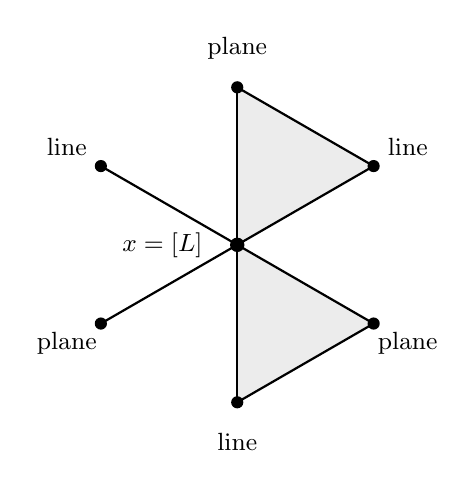
\begin{tikzpicture}[scale=1.0,>=Latex]
  \coordinate (O) at (0,0);
  \foreach \a in {90,30,-30,-90,-150,150} {
    \path (O) ++(\a:2.0) coordinate (P\a);
  }
  \fill[gray!15] (O) -- (P90) -- (P30) -- cycle;
  \fill[gray!15] (O) -- (P-30) -- (P-90) -- cycle;
  \draw[thick] (P90) -- (P30);
  \draw[thick] (P-30) -- (P-90);
  \foreach \a/\lab in {90/{plane},30/{line},-30/{plane},-90/{line},-150/{plane},150/{line}} {
    \draw[thick] (O) -- (P\a);
    \fill (P\a) circle (2.2pt);
    \node[font=\small] at ($(P\a)+(\a:0.5)$) {\lab};
  }
  \fill (O) circle (2.6pt);
  \node[font=\small] at (-0.95,0) {$x=[L]$};
\end{tikzpicture}
\caption{A local view of the affine $\widetilde A_2$ building near a hyperspecial vertex. The neighbors come in two types (lines and planes in the residue-space quotient), and each chamber through $x$ corresponds to an incident line--plane pair.\label{fig:new-local-link}}
\end{figure}


For a regular semisimple $h\in H(F)$, an ordinary orbital integral is
an integral of $f(x^{-1}hx)$ over $H_h(F)\backslash H(F)$.
Given an automorphism $\sigma$ of $G(F)$, a twisted orbital integral
integrates $\phi(x^{-1}g\sigma(x))$ over the corresponding twisted
centralizer quotient. Distinct rational twisted classes can lie in one
stable twisted class. The comparison of such orbital integrals needs
transfer factors and consistent measures, not merely equality of
unweighted numbers of lattices.

With $K=G(\mathcal O_F)$, the spherical Hecke algebra
$\mathcal H(G,K)$ consists of compactly supported $K$-bi-invariant
functions under convolution. Its unit is $1_K$ when
$\operatorname{vol}(K)=1$. The Satake transform identifies this
commutative algebra with Weyl-invariant functions on a dual torus.
Pullback through an $L$-homomorphism determines the corresponding
spherical function on an endoscopic group.

\begin{example}[An elementary normalization]
For $F=\mathbb Q_3$, the link of the standard $PGL_3$ vertex is the
incidence graph of $PG(2,3)$. Its $52$ complete flags correspond to
$52$ chambers through that vertex. Thus a spherical-to-Iwahori
normalization already introduces a factor $52$, even before one
counts any fixed vertices of a twisted transformation.
\end{example}



The rest of this section is organized as follows.
Subsections~\ref{sec:1}--\ref{sec:1.4} recall the adjoint lifting, the
Jacquet--Shalika norm maps, and the statements of the two fundamental
lemmas. Subsections~\ref{sec:4} and \ref{sec:5} contain the two
historical accounts of building geometry: Langlands' comparison with
$SL(2)$, and the comparison with $PGL(2)$ of \cite{Jo90}. These two
subsections use the reductions of Section~\ref{sec:3}, which the
reader may consult first. Statements are numbered consecutively within
each section; the numbering of \cite{Jo90} is not preserved, and a
concordance is given in the revision log.

\begin{runex}[The two buildings over $\mathbb Q_3$]
\label{run:background}
In the notation of Subsection~\ref{sec:intro-running}, the tree of
$PGL_2(\mathbb Q_3)$ is $4$-regular. The four neighbors of
$[\Lambda_0]$ are the classes of the lattices
$\mathbb Z_3v+3\Lambda_0$, where $v$ runs over the four points
$e_1$, $e_2$, $e_1+e_2$, $e_1-e_2$ of the projective line over
$\mathbb F_3$:
\[
 p''=[\mathbb Z_3e_1+3\mathbb Z_3e_2],\quad
 p'=[3\mathbb Z_3e_1+\mathbb Z_3e_2],\quad
 q_\pm=[\mathbb Z_3(e_1\pm e_2)+3\Lambda_0].
\]
All four have type $1$ modulo $2$, and $[\Lambda_0]$ has type $0$.
In the building of $PGL_3(\mathbb Q_3)$ the vertex $[L_0]$ has
$13+13=26$ neighbors, one for each line and each plane of
$L_0/3L_0=\mathbb F_3^3$, and lies on $52$ chambers. For instance
$[3\mathbb Z_3e_0\oplus\Lambda_0]$ is the neighbor attached to the
plane spanned by $e_1,e_2$, and
$[\mathbb Z_3e_0\oplus3\Lambda_0]$ is the neighbor attached to the
line spanned by $e_0$.
\end{runex}

\subsection{The adjoint lifting: history}
\label{sec:1}

Let $F$ denote a $p$--adic field and $\Pi (G(F))$ denote the set of
equivalence classes of admissible irreducible representations of $G(F)$,
for a 
reductive algebraic group $G$ defined over $F$. 
Typically, $F$ will be a completion of a
number field $K$ at a place $v$; let $\aaa = \aaa_K$ denote the adele ring 
of $K$.
 
One example of the local functoriality conjecture (\cite{Bo79}, \cite{La80a})
says that the 
$L$--homomorphism

\begin{equation}
\label{eqn:1.1}
r : GL(2,\ccc ) \rightarrow GL(2n+1,\ccc ),
\end{equation}
given by $r := \operatorname{Sym}^{2n}(\mathrm{Std})\otimes (\det)^{-n}$ should 
yield a transfer (the ``symmetric $(2n)$th-power lifting'')

\begin{equation}
\label{eqn:1.2}
r_* : \Pi (GL(2,F)) \rightarrow \Pi (GL(2n+1,F)) .
\end{equation}
Using $L$--parameters one can directly ``lift'' or transfer unramified
principal series from $GL(2,F)$ to $GL(2n+1,F)$, so there is some evidence
for the validity of this conjecture. There is of course a global analog
of this conjectural transfer, predicted by the global functoriality
principle. 
 
If $n=1$ then S. Gelbart and H. Jacquet \cite{GJ78} proved the existence
of a global representation $\Pi \in \Pi (GL(3,\aaa ))$ associated
to a cuspidal $\pi \in \Pi (GL(2,\aaa ))$ using the theory of $L$--functions,
converse Hecke theory on $GL(3,\aaa )$ \cite{JPS79}, and an idea of
G. Shimura \cite{Sh75}. Let me reformulate this in terms of functoriality: 
when $n = 1$, the $L$--map (\ref{eqn:1.1}) becomes

\begin{equation}
\label{eqn:1.3}
r\left(\smallmatrix a&b \\ c&d \endsmallmatrix\right)
= {1\over{ad-bc}}\left(\smallmatrix a^2&-ab&-b^2 \\
-2ac&ad+bc&2bd\\
-c^2&cd&d^2 \endsmallmatrix\right)
\end{equation}
the adjoint representation of $sl(2,\ccc )$ with respect to the basis

\[
\underline{e}_1 := \left(\smallmatrix 0&1 \\ 0&0 \endsmallmatrix\right),
\ \underline{e}_2 := \frac12\left(\smallmatrix 1&0 \\ 0&-1 \endsmallmatrix\right),
\ \underline{e}_3 := \left(\smallmatrix 0&0 \\ 1&0 \endsmallmatrix\right),
\]
and this factors through $PGL(2)$ giving us

\begin{equation}
\label{eqn:1.4}
\lambda_1 :  {^{L}SL(2,\ccc )} =PGL(2,\ccc )
\hookrightarrow SO(3,\ccc ) 
\hookrightarrow  SL(3,\ccc ) = {^{L}PGL(3,\ccc )} .
\end{equation}
The functoriality conjecture then predicts a local and global transfer
from $SL(2)$ to $PGL(3)$. On the other hand, the natural embedding gives us
an $L$--map

\begin{equation}
\label{eqn:1.5}
\lambda_2 : {^{L}PGL(2,\ccc )} \hookrightarrow {^{L}PGL(3,\ccc )},
\end{equation}
In this case the functoriality conjecture predicts a local and global
transfer from $PGL(2)$ to $PGL(3)$. The global transfer associated to 
(\ref{eqn:1.5}) 
is in fact the Gelbart--Jacquet lift. The local transfer associated to
(\ref{eqn:1.4}) will be elaborated upon in subsection 
\ref{sec:1.2} below.
 
Around 1976, H. Jacquet suggested that there should be a twisted trace
formula for $PGL(3)$, corresponding to the outer automorphism

\[
\sigma : g \longmapsto J{^{t}g^{-1}}J,\ \ \sigma^2 = 1,
\]
where $J$ is the involutory matrix ($J^2=I$) given by

\[
J:= \left(\smallmatrix \ &\ &1\\
\ &-1&\ \\
1&\ &\ \endsmallmatrix\right),
\]
and that this trace formula could be applied to proving the symmetric square 
transfer in a fashion analogous to the base change lift of 
Saito--Shintani--Langlands.  Moreover,
$PGL(2)$ and $SL(2)$ should be $\sigma$--endoscopic groups for $PGL(3)$ and the
symmetric square transfer should be a consequence of stabilizing this twisted
$PGL(3)$-trace formula. The notes \cite{LaUn}, completed a year or so later,
were motivated by Jacquet's suggestion.

\subsection{$L$--parameters and the transfer from $SL(2)$ to $PGL(3)$}
\label{sec:1.2}

Let $F$ be a $p$--adic field with ring of integers $\off$, let $G$
denote one of the groups $SL(n)$ or $PGL(n)$, let $K$ denote
a maximal compact subgroup of $G(F)$, and let $\hhh (G,K)$
denote the {\bf Hecke algebra} of compactly
supported locally constant functions on the double coset space
$K\setminus G(F)/K$. Let $K_0:= G(\off )$ denote the hyperspecial
maximal compact subgroup; when $K = K_0$, we write $\hhh (G) := 
\hhh (G,K_0)$. Let $C^\infty_c(G)$ denote the algebra of 
{\bf Schwartz--Bruhat functions} of locally constant functions of
compact support on $G(F)$. 
 
Corresponding to the $L$--map (\ref{eqn:1.4}), the Satake transform (defined 
in \S \ref{sec:2} below) gives us a homomorphism of Hecke algebras

\begin{equation}
\label{eqn:1.6}
\begin{split}
&\lambda_1^* : \hhh (PGL(3)) \rightarrow \hhh (SL(2)),\\
&\ \ \ \ \ \ \ \ \ \ \ \phi \longmapsto f :=\lambda_1^*(\phi),
\end{split}
\end{equation}
determined by 
$\hat{f}(t) = \hat{\phi }(\lambda_1 (t)),\ t \in {^{L}SL(2,\ccc )}$.
When this identity holds, one says that the spherical function $\phi $
on $PGL(3,F)$ {\bf corresponds} with the spherical function $f$ on $SL(2,F)$.
Similarly, corresponding to the $L$--map (\ref{eqn:1.5})
there is the $L$--homomorphism of Hecke algebras

\begin{equation}
\label{eqn:1.7}
\begin{split}
&\lambda_2^* : \hhh (PGL(3)) \rightarrow \hhh (PGL(2)),\\
&\ \ \ \ \ \ \ \ \ \ \ \phi \longmapsto f := \lambda_2^*(\phi),
\end{split}
\end{equation}
determined by $\hat{f}(t) = \hat{\phi }(\lambda_2 (t)),\ t \in 
{^{L}PGL(2,\ccc )}$. Using this one can define a ``correspondence'', as above,
between spherical functions on $PGL(3,F)$ and spherical functions on
$PGL(2,F)$. 
 
According to the local Langlands correspondence for $SL(2)$, to each
unramified admissible homomorphism
$\theta :W_F \rightarrow {^{L}SL(2,\ccc )}$ there is an $L$--packet of
admissible irreducible 
unramified representations $\Pi (\theta )  \in
\Pi (SL(2,F))_L$ of SL(2,F). Here $W_F$ denotes the 
absolute local Weil group of $F$ and the subscript $L$ on the $\Pi$ signifies
that we are identifying $L$--indistinguishable representations. 
Each homomorphism
$\theta : W_F \rightarrow {^{L}SL(2,\ccc )}$ yields via (\ref{eqn:1.4})
a homomorphism $\theta^* : W_F \rightarrow {^{L}PGL(3,\ccc )}$, and if 
$\theta$ is
admissible then so is $\theta^*$. The local functoriality conjecture
predicts that the $L$--map (\ref{eqn:1.4}) 
should yield a map of tempered $L$--packets

\begin{equation}
\label{eqn:1.8}
\begin{split}
&\Lambda_1 : \Pi^{\text{temp}}(SL(2,F))_L \rightarrow 
\Pi^{\text{temp}}(PGL(3,F)),\\
&\quad\quad \ \ \ \ \ \ \ \ \ \ \Pi (\theta ) \longmapsto \pi_{\theta^*}.
\end{split} 
\end{equation}
We say that $\pi \in \Pi (SL(2,F))$ {\bf transfers} to 
$\Pi \in \Pi (PGL(3,F))$ if $\pi \in \Pi (\theta )$ and 
$\Pi = \pi_{\theta^*}$, for some admissible $\theta$ as above. 
The $L$--packets of $SL(2)$ have been described by J.-P. Labesse
and R. Langlands \cite{LL79}.

\subsection{The Jacquet--Shalika norm maps}
\label{sec:1.3}

The basic ideas of this subsection are, I believe, due to H. Jacquet
and J. Shalika and may be found in \cite{LaUn}.
 
Let $G := PGL(3),\ H_1 := SL(2),\ H_2 := PGL(2)$.
Associated to the two $\sigma$-endoscopic groups $H_i$ are ``norm'' maps

\begin{equation}
\label{eqn:1.9}
N_i : \{\text{stable $\sigma$-conjugacy classes in G}\} \rightarrow
\{\text{stable conjugacy classes in $H_i$}\},
\end{equation}
which (hopefully) allow one to relate stable class functions on $G$ to stable
class functions on $H_i$. The explicit construction of these norm maps
is the object of this subsection.

\begin{lemma}
\label{lemma:1.10}
Let $[C]\in PGL(2n+1,F)$, with $C\in GL(2n+1,F)$, and take an
involutory skew-diagonal matrix $J$ of the same size. Put $A=CJ$.
For $\sigma_J([C])=[J\,{}^tC^{-1}J]$, the product
$[C]\sigma_J([C])$ is represented by
$A\cdot{}^tA^{-1}$, and this matrix has at least one
 eigenvalue equal to one.
\end{lemma}
 
Indeed, $C\sigma_J(C)=CJ\,{}^tC^{-1}J=A\,{}^tA^{-1}$.
The skew-symmetric matrix $A^{-1}-{}^tA^{-1}$ is singular
in odd dimension. Thus $A\,{}^tA^{-1}$ has eigenvalue $1$.
In the norm-map computations below, $A$ always denotes this
\emph{normalized representative} $CJ$. In contrast, $C$ denotes a
literal representative of the original $\sigma_J$-twisted class.
This change of representative corresponds to writing the geometric
action with the equivalent involution $\tau(x)={}^tx^{-1}$; it does
not change the definition of $\sigma_J$.
 
Let $V:=F^{2n+1}$ and identify, by fixing a basis of $V$, $GL(2n+1,F)$ with 
$\text{Aut}_F(V)$. For the $[A]$ and $A$ in the lemma, let 
$V_A \subset V$ be a 1-dimensional subspace on which $A\cdot {^{t}A^{-1}}$
acts as the identity. Let $W_A$ be the orthogonal complement of
${^{t}A^{-1}}V_A$ with respect to the inner product 
$(v_1,v_2) := {^{t}v_1\cdot v_2}$.
Observe that $A\cdot {^{t}A^{-1}}$ acts on $V_A$ trivially, 
therefore on $V/V_A$, and
$A{^{t}A^{-1}}$ acts on $W_A$. 
 
Let me now restrict to the case $n = 1$.

\begin{lemma}
\label{lemma:1.11} 
Suppose that $A\cdot {^{t}A^{-1}}$ induces the linear transformation
$B_1 \in \text{Aut}_F(W_A)$ and $B_2 \in \text{Aut}_F(V/V_A)$. Then

\begin{itemize}

\item[(a)] 
$\det B_1 = \det B_2 = 1$,

\item[(b)] 
there is an isomorphism $\theta : W_A \rightarrow V/V_A$ such that

\[
\begin{CD}
W_A @>B_1>>W_A\\
@V\theta VV @AA\theta A\\
V/V_A @>B_2>>V/V_A
\end{CD}
\]
commutes,

\item[(c)] 
as elements of $SL(2,F)$, $B_1$ and $B_2$ are stably conjugate,

\item[(d)] 
the stable conjugacy class of $B_i$ is independent of the choice 
of $V_A$.
\end{itemize}
\end{lemma}
 
For the proof, I refer to \cite{LaUn}.

\begin{definition}
\label{def:1.12} 
Choose a basis of $V/V_A$ or of $W_A$ and represent
the transformation induced by $A\cdot {^{t}A^{-1}}$ by a 
$2\times 2$ matrix. The stable
$SL(2)$-conjugacy class of this matrix is 
well--defined and depends only on the 
stable $\sigma$--conjugacy class of $[A]$. 
This stable conjugacy class in
$SL(2,F)$ is called the {\bf $H_1$-norm} of $[A]$, written as
$N_1([A]) \subseteq H_1(F)$. For the $H_2$--norm, first identify
$H_2$ with SO(3) via the adjoint representation (\ref{eqn:1.3}), 
where $SO(3)$ denotes the connected component of the orthogonal group for the 
skew--diagonal matrix $J$ above. If the eigenvalues of
$A\cdot {^{t}A^{-1}}$ are $\alpha,\ 1,\ \alpha^{-1}$ and 
$\alpha \not= \pm 1$, then
define the {\bf $H_2$--norm} of $[A]$, written $N_2([A])$, to be the
stable $H_2$--conjugacy class which contains a matrix with
$\alpha,\ 1,\ \alpha^{-1}$ as eigenvalues.
\end{definition}
 
As a matter of notation, let

\[
\begin{split}
&Cl^{st}_{\sigma}(G) :=\{\text{stable $\sigma$-conjugacy classes in G}\},\\
&Cl^{st}(H_i) := \{\text{stable conjugacy classes in $H_i$}\}.
\end{split}
\]

\begin{proposition} (Jacquet--Shalika)
\label{prop:1.13} 
The norm map

\[
N_1 : Cl^{st}_{\sigma}(G) \rightarrow Cl^{st}(H_1)
\]
is a bijection.
\end{proposition}

\begin{remark} 

(1) This is proven in \cite{LaUn} by explicit
matrix manipulations.
\newline

(2) For $H_2$ stable conjugacy and ordinary conjugacy
are essentially the same, so the statement analogous to the 
proposition is false for $N_2$. 
\newline

(3) In general, one expects to be able to define norms from PGL(r) to
any of its $\sigma$--endoscopic groups. One expects that the norm map
associated to the ``largest'' $\sigma$--endoscopic group should also yield a
bijection. For r = 2n+1 and r = 2n, one would like bijections

\[
\begin{split}
&N: Cl^{st}_{\sigma}(PGL(2n+1)) \rightarrow Cl^{st}(Sp(2n)),\\
&N: Cl^{st}_{\sigma}(PGL(2n)) \rightarrow Cl^{st}(PSp(2n)).
\end{split}
\]
\end{remark}
 
The following corollary of Langlands' proof of (\ref{prop:1.13}) 
is sometimes useful.

\begin{corollary}
\label{cor:1.14} 
If $N_1([A])$ does not contain a unipotent, then 
there is a $[A']$ in the same stable $\sigma$--conjugacy class 
as $[A]$ and 
represented by $A' \in GL(3,F)$, for which

\begin{itemize}

\item[(a)] 
$V = V_{A'} \oplus W_{A'}$,

\item[(b)] 
$W_{A'}^{\bot} = V_{A'}$ with respect to the inner product
$(v_1,v_2):={^{t}v_2}\cdot v_1$,

\item[(c)] 
$V_{A'}$ and $W_{A'}$ are both invariant under $A$ and 
${^{t}A^{-1}}$ (i.e., $A$ can be put in $(2,1)$-block form).
\end{itemize}
\end{corollary}


\begin{runex}[The two norms]
\label{run:norm}
For the matrices $A_a=\operatorname{diag}(a,C)$ of
\eqref{eq:run-Aa} one has
$A_a\,{}^tA_a^{-1}=\operatorname{diag}(1,h)$, so the eigenvalue $1$
of Lemma~\ref{lemma:1.10} is visible and $V_A=Fe_0$. Since
${}^tA_a^{-1}V_A=Fe_0$, the space $W_A$ is the orthogonal complement
$Fe_1\oplus Fe_2$ of $e_0$, and $V=V_A\oplus W_A$ as in
Corollary~\ref{cor:1.14}. The transformation induced on $W_A$ is $h$,
so $N_1([A_a])$ is the stable class of $h$ in $SL_2(\mathbb Q_3)$.
In specimen~I, for example,
\[
 C=\smat{-1}{-1}{1}{-1},\qquad
 {}^tC^{-1}=\tfrac12\smat{-1}{-1}{1}{-1}=\tfrac12C,\qquad
 h=\tfrac12C^2=\smat{0}{1}{-1}{0},
\]
and the skew-symmetric matrix of Lemma~\ref{lemma:1.10} is
$A_1^{-1}-{}^tA_1^{-1}=\operatorname{diag}\bigl(0,\smat{0}{1}{-1}{0}\bigr)$,
with kernel $Fe_0$. The eigenvalues of $A_a\,{}^tA_a^{-1}$ are
$\beta_1,1,\beta_1^{-1}$. An element of $PGL_2$ whose two eigenvalues
have ratio $\beta_1$ maps under \eqref{eqn:1.3} to an element with
these three eigenvalues. The matrix $h'=1+h$ has eigenvalues
$1+\beta_1$ and $1+\beta_1^{-1}$, whose ratio is $\beta_1$, so the
image of $h'$ in $PGL_2(\mathbb Q_3)$ represents $N_2([A_a])$. In
specimen~I this is $h'=\smat{1}{1}{-1}{1}$.
\end{runex}

\subsection{The fundamental lemmas}
\label{sec:1.4}

Recall $G := PGL(3),\ H_1 := SL(2),\ H_2 := PGL(2)$. Let us denote the 
{\bf twisted centralizer} by

\begin{equation}
\label{eqn:1.15}
G(g\sigma ,F) := \{x \in G(F)\ |\ x^{-1}g\sigma (x) = g\},
\end{equation}
and the (ordinary) {\bf centralizer} by

\begin{equation}
\label{eqn:1.16}
H_i(h,F) := \{x \in H_i(F) \ |\ x^{-1}hx = h\},\ \ \ i=1,2.
\end{equation}
Let $\omega_{G(g\sigma )},\ \omega_G$ be fixed nonzero forms of maximal
degree on $G(g\sigma ,F),\ G(F)$, respectively, and let

\[
d\ovx := {d\omega_G(x)\over{d\omega_{G(g\sigma )}(x)}}
\]
denote the quotient measure. For $\phi \in C^\infty_c(G)$, define the 
{\bf twisted orbital integral} by

\begin{equation}
\label{eqn:1.17}
\Phi (g,\phi ,\omega_G,\omega_{G(g\sigma )}) = \Phi (g,\phi )
:= \int_{G(g\sigma ,F)\setminus G(F)}
\phi (x^{-1}g\sigma (x))\ d\ovx,
\end{equation}
provided it converges.
Similarly, let $\omega_{H_i(h)},\ \omega_{H_i}$ be fixed nonzero 
forms of maximal
degree on $H_i(h,F),\ H_i(F)$, respectively, and let

\[
d\ovx := {d\omega_{H_i}(x)\over{d\omega_{H_i(h)}(x)}}
\]
denote the quotient measure. In fact, we don't take any $\omega_{H_i(h)}$,
but only one obtained by pulling back $\omega_{G(g\sigma)}$ via an \'etale
surjective homomorphism over $\overline{F}$

\[
\psi_i : H_i(h)^0 \rightarrow G(g\sigma ),
\]
namely, it must satisfy

\[
\omega_{H_i(h)}=|\text{ker }\psi_i|^{-1}\psi^*_i\omega_{G(g\sigma )},
\]
for all $h \in N_i(g)$. Here $N_i$ denotes the norm map defined above. 
Note that if $h \in H_i(F)$ is regular semi--simple then we may assume that
$\psi_i$ is an isomorphism. For $f \in C^\infty_c(H_i)$ and $h \in H_i(F)$
regular, define the {\bf orbital integral} by

\begin{equation}
\label{eqn:1.18}
\Phi (h,f,\omega_{H_i},\omega_{H_i(h)}) = 
\Phi (h,f):= \int_{H_i(h,F)\setminus H_i(F)}
f(x^{-1}hx)\ d\ovx .
\end{equation} 
This defines the orbital integrals which will
occur in the fundamental lemmas below. Note that, whereas 
$\Phi (h,f)$ is a class function on $H_i(F)^{reg}$, $\Phi (g,\phi )$
may be regarded as a class function on the nonconnected reductive group

\[
\overline{G} := G \rtimes \{1,\sigma \},\ \ {\rm (semi-direct\ product)},
\]
because of the identity

\[
(x\times \sigma )^{-1}(g\times \sigma )(x\times \sigma )
=\sigma (x^{-1}g\sigma (x))\times \sigma .
\]
 
To analyze these integrals further we of course should know something
about the conjugacy classes on $H_i$ and on $\overline{G}$. Actually,
from now on I shall pretty much ignore $\overline{G}$ since it
seems easier to regard conjugacy classes on
$\overline{G}$ as $\sigma$--conjugacy classes on $G$. 
 
Let me leave aside the notion of $\sigma$-conjugacy for the moment
and first discuss the (untwisted) notions of conjugacy and
stable conjugacy. Two elements
$h_1,\ h_2 \in SL(2,F) = H_1(F)$ can be {\bf stably conjugate}
(meaning that there is an $x \in H_1(\ovF )$ such that
$h_1 = x^{-1}h_2x$) but not conjugate (over $F$). 
This is not true for $PGL(n)$. 
In other words, if two elements of $PGL(n,F)$ are
$PGL(n,\ovF )$-conjugate then they are necessarily
$PGL(n,F)$-conjugate (see, for example, \cite{La84}, ch. 15, \S 3, p. 543).
Equivalently, for $PGL(n)$, the notions of stable 
conjugacy and (ordinary) conjugacy coincide. 
For groups other than
$PGL(n)$, however, these notions do not generally coincide. 
As a measure of the 
difference between these two notions, one may consider the set
of conjugacy classes of an element within a given stable conjugacy class
of that element. 
For $h \in H_i(F)$, the set of $H_i(F)$-conjugacy
classes of $h_i$ within the stable conjugacy class of $h$ is parameterized 
by 

\begin{equation}
\label{eqn:1.19}
\ddd (h,H_i) := H_{i,h}(\ovF )\setminus St(h,H_i)/H_i(F),
\end{equation}
where

\[
St(h,H_i) := \{x \in H_i(\ovF )\ |\ x^{-1}hx \in H_i(F)\}
\]
denotes those elements over $\ovF$ which leave invariant the
stable conjugacy class of $h \in H_i(F)$ under conjugation. 
If $i = 2$ then
$\ddd (h,H_2)$ is a singleton since in that case the notions of 
stable conjugacy and ordinary conjugacy coincide. 
 
Now let me turn to the twisted analogs of these notions. Although
$PGL(n)$ has ``no $L$--indistinguishabilty'' it \underbar{does} have
``twisted 
\newline
$L$--indistinguishability''. In other words, it is
possible for $g_1,\ g_2 \in G(F)$ to be stably $\sigma$-conjugate
(meaning that there is some $g\in G(\ovF )$ such that
$g_1 = g^{-1}g_2\sigma (g)$) but not $\sigma$-conjugate over $F$.
For $g \in G(F)$, the set of $\sigma$-conjugacy classes of $g$ within the
stable $\sigma$-conjugacy class of $g$ is parameterized by

\begin{equation}
\label{eqn:1.20}
\ddd_{\sigma}(g,G) := G_{g\sigma}(\ovF)\setminus St_{\sigma}(g,G)/G(F),
\end{equation}
where

\[
St_{\sigma}(g,G) := \{x \in G(\ovF )\ |\ x^{-1}g\sigma(x) \in G(F)\}
\]
denotes those elements over $\ovF$ which leave invariant the 
stable $\sigma$-conjugacy class of $g$.

\begin{lemma}
\label{lemma:1.21} 
There are isomorphisms (as pointed sets)

\[
\begin{split}
&\ddd (h, H_i) \cong
\ker\bigl(H^1(F,H_i(h))\longrightarrow H^1(F,H_i)\bigr),\\
&\ddd_{\sigma}(g,G) \cong
\ker\bigl(H^1(F,G(g\sigma))\longrightarrow H^1(F,G)\bigr).
\end{split}
\]
\end{lemma}
 
This is the usual Galois-descent description of rational orbits in a
stable orbit (see, for example, \cite{La80a}). The kernels, rather than
arbitrary cohomology classes, are the pointed sets corresponding to
rational representatives: a cocycle coming from a rational stable
conjugate becomes trivial after passage to the ambient group.
The simplification to the full $H^1$ in the elliptic calculation of
\eqref{eqn:3.16} must be justified using its particular centralizer. 
We use these kernels to compute the cardinalities below.
 
For a fixed $g\in G(F)$, the twisted centralizers attached to
rational representatives of its stable class are isomorphic over
$\ovF$. For each such representative $g'$, transport the measure on
the centralizer of $g\sigma$ to the centralizer of $g'\sigma$
using a chosen isomorphism. Use the same convention for stable
classes in $H_i$.

If $N_1(g)$ is regular, $g \in G(F)$ then define the {\bf stable twisted 
orbital integral} of $\phi \in C^\infty_c(G)$ by

\begin{equation}
\label{eqn:1.22}
\Phi^{T,1}(g,\phi ):= \sum_{g' \in \ddd_{\sigma}(g,G)} \Phi (g',\phi ),
\end{equation}
where $T$ denotes $G(g\sigma )$.
Similarly, if $h \in H_i(F)$ is regular then define the
{\bf stable orbital integral} of $f \in C^\infty_c(H_i)$ by

\begin{equation}
\label{eqn:1.23}
\Phi^{T_i,1}(h,f):= \sum_{h' \in \ddd(h,H_i)} \Phi (h',f),
\end{equation}
where $T_i$ denotes the centralizer $H_i(h)$.

\begin{theorem} (Langlands,
{\bf Fundamental Lemma for $H_1$})
\label{thrm:fundlemmaH1}
If
$\phi \in \hhh (G)$ and $f_1 = \lambda_1^*(\phi ) \in
\hhh (H_1)$ then, for all non--trivial $h \in N_1(g)$, we have

\begin{equation}
\label{eqn:1.24}
\Phi^{T,1}(g,\phi ) = \Phi^{T_1,1}(h,f_1).
\end{equation}
\end{theorem}
 
We will prove this in \S \ref{sec:4} 
in the case where $\phi$ is the unit element
of $\hhh (G)$ and $p\not= 2$.
 
The analogous statement for $H_2$ requires the introduction
of ``unstable'' orbital integrals. These are the same as stable orbital
integrals except that the sum is ``twisted'' by certain roots of unity
($\pm 1$'s in our case). To define these, we use the property that
the elements $g \in G(F)$ with $N_1(g) = 1$ have the property
that $|\ddd_{\sigma}(g,G)|=2$, and we can define a bijection of sets

\begin{equation}
\label{eqn:1.25}
\kappa : \ddd_{\sigma}(g,G) \rightarrow \{\pm 1\},
\end{equation}
by

\[
\kappa (g) := 
\begin{cases} 
+1,&\ \ \ {\rm if}\ G(g\sigma)\ {\rm is\ split\ over}\ F,\\
-1,&\ \ \ {\rm if}\ G(g\sigma)\ {\rm is\ non--split\ over}\ F .
\end{cases}.
\]
If $N_1(g) \not= 1$ is regular then replace $g$ by $g_{s} :=
(g+{^{t}g})/2$ to get a regular element with $N_1(g_{s})=1$. In this
case, define $\kappa (g) = \kappa (g_{s})$. This depends only
on the $\sigma$-conjugacy class of $g$. This sign is closely related
to the Hilbert norm residue symbol of $E/F$, where $E$ is the quadratic
extension obtained from adjoining the eigenvalues of $h \in N_1(g)$ to
$F$, see \S \ref{sec:4} below. 
The {\bf unstable or $\kappa$-orbital integral}
of $\phi \in C^\infty_c(G)$ is

\begin{equation}
\label{eqn:1.26}
\Phi^{T,\kappa}(g,\phi ):= \sum_{g' \in \ddd_{\sigma}(g,G)} 
\kappa (g')\Phi (g',\phi ),
\end{equation}
where $T:=G(g\sigma )$.

\begin{conjecture}
({\bf Fundamental Lemma for $H_2$})
Assume $N_2(g) \not= 
\pm 1$. If $\phi \in \hhh (G)$ and $f_2:=\lambda_2^*(\phi ) \in
\hhh (H_2)$ then, for any $h \in N_2(g)$, we have

\begin{equation}
\label{eqn:1.27}
\Phi^{T,\kappa}(g,\phi ) = \tau (g)\Phi(h,f_2),
\end{equation}
where $\tau$ is the transfer factor
\[
\tau (h) := \pm |(1+\beta_{1})(1+\beta_{2})|^{1/2},
\]
denoting the eigenvalues of $h$ by $\beta_{1},\ \beta_{2}$. The $\pm$ sign
will be explained in (\ref{eqn:3.18}) below.
\end{conjecture}
 
This main result of this paper is, as mentioned earlier, the proof that
this holds when the residual characteristic of $F$ is greater than $2$ and
$\phi \in \hhh (G)$ is the unit element. 






% === END ORIGINAL adjoint_lift1.tex ===
% === BEGIN ORIGINAL adjoint_lift2.tex ===

\begin{runex}[The two rational classes and the sign $\kappa$]
\label{run:kappa}
Twisted conjugation by $x^{-1}$ replaces a normalized representative
$A$ by $xA\,{}^tx$. With $x=\operatorname{diag}(\sqrt a,1,1)$ this
carries $A_1$ to $A_a$, so all the $A_a$ of \eqref{eq:run-Aa} lie in
one stable class. By Proposition~\ref{prop:new-Zfix}(d), $A_a$ and
$A_b$ are $\sigma$-conjugate over $F$ when $a/b\in N_{E/F}(E^\times)$.
For the unramified specimens, $N_{E/F}(E^\times)=3^{2\mathbb Z}\mathbb Z_3^\times$,
and $A_1$, $A_3$ are not $\sigma$-conjugate over $F$: their numbers
of fixed vertices differ (Lemma~\ref{lemma:4.4}), and so do their
signs $\kappa$ below. So $A_1$ and
$A_3$ represent the two elements of $\ddd_\sigma(g)$ in
\eqref{eqn:3.16}. For specimen~IV one may take $A_1$ and $A_2$, since
$2$ is not a norm from $\mathbb Q_3(\sqrt3)$.

The sign $\kappa$ of \eqref{eqn:1.25} is computed from the symmetric
part $(A_a+{}^tA_a)/2=\operatorname{diag}(a,C_s)$, where
$C_s=(C+{}^tC)/2$: the twisted centralizer of a symmetric matrix is
its special orthogonal group, which is split exactly when the ternary
quadratic form is isotropic.
\begin{center}
\small
\renewcommand{\arraystretch}{1.25}
\begin{tabular}{@{}clcc@{}}
\toprule
 & form of $(A_a+{}^tA_a)/2$ & isotropic for & $\kappa$\\
\midrule
I & $ax^2-y^2-z^2$ & $a=1$ & $\kappa(A_1)=+1$, $\kappa(A_3)=-1$\\
II & $ax^2-y^2-3yz-z^2$ & $a=1$ & $\kappa(A_1)=+1$, $\kappa(A_3)=-1$\\
III & $ax^2-3y^2-3z^2$ & $a=3$ & $\kappa(A_1)=-1$, $\kappa(A_3)=+1$\\
IV & $ax^2+3y^2-z^2$ & $a=1$ & $\kappa(A_1)=+1$, $\kappa(A_2)=-1$\\
\bottomrule
\end{tabular}
\end{center}
The reasons are short. Because $-1$ is not a square modulo $3$, the
form $y^2+z^2$ takes only values of even valuation on nonzero vectors;
hence $3x^2=y^2+z^2$ and $x^2=3(y^2+z^2)$ have no nonzero solutions,
while $x^2-y^2-z^2$ vanishes at $(1,1,0)$. In specimen~II the form
with $a=1$ is unimodular of rank three over $\mathbb Z_3$, hence
isotropic, and with $a=3$ it is anisotropic because $y^2+3yz+z^2$ has
unit discriminant $5$, a nonsquare. In specimen~IV, $x^2-z^2$ is
hyperbolic; for $a=2$, which is $-1$ times a square, the form is
equivalent to $-x^2+3y^2-z^2$, which is anisotropic.

Note that $\kappa(A_1)=+1$ in specimens I and II and
$\kappa(A_1)=-1$ in specimen~III. So in the labeling $a\mapsto A_a$,
the relation between $\kappa(A_a)$ and the Hilbert symbol
$(a,\epsilon)_2=(-1)^{v_F(a)}$ depends on the specimen; see
Remark~\ref{rem:sign-evidence}.
\end{runex}

\subsection{The buildings for $PGL(3)$ and $SL(2)$}
\label{sec:4}

For background, see for example \cite{Ko80} and \cite{Ti79}.
The results (and pictures) in this section are, as 
mentioned earlier, due to R. Langlands
\cite{LaUn}. We assume $p\not= 2$ throughout this section.
 
Fix a vector space $V$ over $F$ of dimension either 2 or 3.
We may consider the buildings $\bbb (G),\ \bbb (H_1)$ for $G,\ H_1$
as graphs of lattice classes; if L is a rank two or three $\off$--lattice
in $V$
then its class is denoted by [L]. Recall that two vertices $[L_1],\ [L_2]$
are to be joined by an {\bf edge} if and only if there exist 
$\lambda_1,\ \lambda_2 \in F^{\times}$ such that

\begin{equation}
\label{eqn:4.1}
\pi\lambda_1 L_1 \sne \lambda_2 L_2 \sne \lambda_1 L_1.
\end{equation}
The edge from $[L_2]$ to $[L_1]$ is {\bf positively directed} if \eqref{eqn:4.1}
holds and if $\lambda_1 L_1/\lambda_2 L_2$ is a module of rank one
over the residue field.
Three vertices $L_1,\ L_2,\ L_3$ are the vertices of a 2-simplex
or {\bf chamber} of $\bbb (G)$ if and only if there exists
$\lambda_1,\ \lambda_2,\ \lambda_3 \in F^{\times}$ such that

\begin{equation}
\label{eqn:4.2}
\pi\lambda_1 L_1 \sne \lambda_3L_3 
\sne \lambda_2 L_2 \sne \lambda_1 L_1.
\end{equation}
 
To describe the ordinary action of $G$ on
$\bbg$, represent $g\in G(F)$ by $C\in GL(3,F)$.
The scalar center $Z(GL_3)(F)=F^\times$ acts trivially on
homothety classes, so this action is well-defined and given by
$g:[L]\mapsto[CL]$.
The action of $H_1$ on $\bbH1$ is simpler: $h\in H_1(F)$ sends
$[\Lambda ]$ to $[h\Lambda ]$. These actions send vertices to vertices, 
edges to edges, chambers to chambers
(in the case of $\bbg$), preserve orientation and are
automorphisms of the buildings. 
 
The action of $\sigma$ on $\bbg$, however, does not preserve orientation.
This ``anti--automorphism'' sends a lattice $L$ to its dual lattice

\begin{equation}
\label{eqn:4.3}
\check{L} :=\{v \in V\ |\ {^{t}v}\cdot v' \in \off , \ \forall v' \in L\}.
\end{equation}
If $[L]=[C_0\off^3]$, then the original involution
$\sigma_J(C)=J\,{}^tC^{-1}J$ acts on vertices by
\[
\sigma_J:[L]\longmapsto[J\check L],
\]
since $J\off^3=\off^3$. If $g=[C]$, put $A=CJ$. Then
$g\sigma_J$ acts by $[L]\mapsto[A\check L]$.
We retain the historical shorthand $A\sigma$ for this
\emph{normalized building action}. Equivalently, this is $A\tau$
with $\tau(C)={}^tC^{-1}$. In subsequent geometric formulas $A$ is
normalized, not the literal representative $C$ of $g$.
It is the fixed-point set of this action that we describe.

\begin{lemma}
\label{lemma:4.4} 
\begin{itemize}

\item[(a)] 
Suppose that the number of fixed points of 
$h\in H_1(F)$ in $\bbH1$ is finite: $|{\rm Fix}(h)| < \infty$. 
(This is the case if
$h$ is elliptic regular, i.e., the eigenvalues of $h$ generate a quadratic
extension of $F$.) Then, for any $x\in H_1(F)$, we have 
$|{\rm Fix}(h)| =|{\rm Fix}(x^{-1}hx)|$,
i.e., the number of fixed points depends only on the conjugacy class of $h$.

\item[(b)] 
Suppose that the number of fixed points of $g\sigma$ in $\bbg$ is
finite: $|{\rm Fix}(g\sigma )|<\infty$. (This is the case if $N_1(g)$ is 
elliptic regular.) Then, for any $x\in PGL(3,F)$, we have 
$|{\rm Fix}(g\sigma )| = |{\rm Fix}((x^{-1}g\sigma (x))\sigma )|$,
i.e., the number of fixed points of $g\sigma$ depends only on the
$\sigma$--conjugacy class of $g$.
\end{itemize}
\end{lemma}

\begin{remark}
The proof of this lemma is easy, hence is omitted. 
If $h,\ h'$ are stably conjugate but not conjugate over $F$ one
may have $|{\rm Fix}(h)|\not= |{\rm Fix}(h')|$, 
and a similar statement holds for
$\sigma$--conjugacy.
\end{remark}
 
The following result is well-known. 

\begin{lemma}
\label{lemma:4.5} 
Let $h\in GL(2,F)$ be an elliptic regular element
with $\Delta_{H_2} (h)=q^{-k}$, for some $k\geq 0$. Let $E/F$ denote the
quadratic extension generated by $h$. 

\begin{itemize}
\item 
If $E/F$ is unramified then

\[
|{\rm Fix}(h)|={{q^{k+1}+q^k-2}\over{q-1}}.
\]        
\item 
If $E/F$ is ramified then

\[
|{\rm Fix}(h)|={2(q^k-1)\over{q-1}}.
\]        
(We have used the fact that the conductor of $E/F$, as defined in \cite{Bl85},
is $1$ in the ramified case.)
\end{itemize}
\end{lemma}

We now describe an embedding

\[
\bbb (H_1) \hookrightarrow \bbb (G).
\]
First, replace the tree $\bbb (H_1)$ by the product of itself with 
the affine line:
replace all vertices by lines (copies of $V_A$ running perpendicular to the 
edges, as visualized in three dimensions) and all edges by strips. 
This figure may be regarded as $\bbb (GL(2))$. 
In order to embed this into
$\bbb (G)$, one must impose a simplicial structure on it compatible with that
of $\bbb (G)$. 
Each line $\overline{\Lambda}$ of $\bbb (GL(2))$ associated to a
vertex $\Lambda$ of $\bbb (H_1)$ must first be provided with its 
own vertices. 
We define the vertices on $\overline{\Lambda}$ to be 
$\Lambda_{(n)} :=\pi^{-n}\off + \Lambda$,
for fixed embeddings
$\pi^{-n}\off \hookrightarrow V_A,\ \Lambda\hookrightarrow W_A$. 
Here $V_A, \ W_A$ are as in Subsection~\ref{sec:1.3}. Given two neighboring
vertices $\Lambda , \Lambda '$ of $\bbb (H_1)$ we obtain neighboring lines
$\overline{\Lambda},\ \overline{\Lambda '}$ and the vertices of these lines 
are joined by an edge if they are neighbors. 
This simplicial structure 
on $\bbb (GL(2))$ defines an embedding of
$\bbb (H_1)$ into $\bbb (G)$ whose image we denote by $\zz = \zz (V_A,W_A)$. 
Let

\[
\pi\lambda \Lambda \sne \lambda ' \Lambda ' 
\sne \lambda \Lambda ,
\]
and let $L'_{(n)} := \pi^{-n}\off + \Lambda ', 
\ L_{(n)}:=\pi^{-n}\off + \Lambda$. The band in $\zz$ associated to the edge 
joining $\Lambda $ and $\Lambda '$ in $\bbH1$ is represented by a 
picture of the following sort:

%%figure (4.6) on page 1119
\begin{figure}[htbp]
\centering
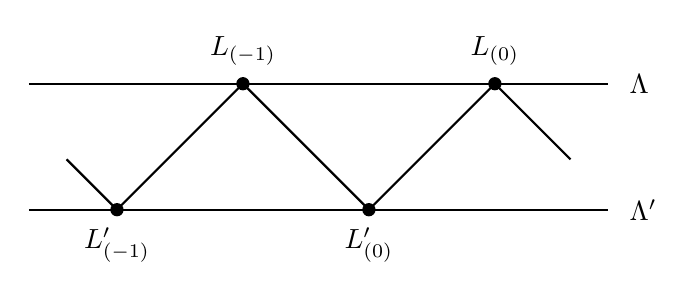
\begin{tikzpicture}[x=0.032cm,y=0.032cm]
  \draw[thick] (-85,50) -- (145,50) node[right=4pt] {$\Lambda$};
  \draw[thick] (-85,0) -- (145,0) node[right=4pt] {$\Lambda'$};
  \draw[thick] (-70,20) -- (-50,0) -- (0,50) -- (50,0) -- (100,50) -- (130,20);
  \foreach \x/\y in {-50/0,0/50,50/0,100/50} { \fill (\x,\y) circle (2.4pt); }
  \node[above=3pt] at (0,50) {$L_{(-1)}$};
  \node[above=3pt] at (100,50) {$L_{(0)}$};
  \node[below=3pt] at (-50,0) {$L'_{(-1)}$};
  \node[below=3pt] at (50,0) {$L'_{(0)}$};
\end{tikzpicture}
\caption{The band in the apartment \label{fig:4.6}}
\end{figure}


\noindent
The lines in $\zz$ have been drawn in such a way that the positive direction 
on them is from left to right. As mentioned earlier, the action of
$\text{Aut}_F(W_A) \hookrightarrow \text{Aut}_F(W_A +V_A)$ on $\zz$ preserves
orientation. 
The action of $\sigma$ on $\bbg$ does not even restrict to an action
on $\zz = \zz (V_A,W_A)$. However, the action of $g\sigma$, with 
$g=[A] \in G(F)$ 
represented by $A \in GL(3,F)$, does send $\zz (V_A, W_A)$ to
$\zz (AW_A^{\bot}, AV_A^{\bot}) = \zz (V_A, W_A)$, reversing orientation. 
Here we have used the fact the $AW_A^{\bot} = V_A$ and 
$AV_A^{\bot}=({^{t}A^{-1}}V_A)^{\bot}$, by definition of $W_A$.
As we shall see, thanks to Corollary \ref{cor:1.14} it turns out 
to be sufficient
for our purpose of relating fixed points of $g\sigma$ 
in $\bbg$ with fixed points
of $h\in N_1(g),\ h\in H_1(F),$ in $\bbH1$ to assume that the matrix A in
$GL(3,F) \cong \text{Aut}_F(V_A +W_A)$ is in $(1,2)$-block form. 
For such
matrices, it is possible to explicitly realize the action of $g\sigma$
on $\zz$ in terms of the geometry described above. 
In fact, this is what we do next.
 
In \cite{LaUn}, R. Langlands introduced the notion of a ``characteristic
leaf'' to understand explicitly vertices in $\bbg$ not in $\zz$ in terms
of vertices in $\zz$. 
This notion is very useful for relating fixed
points of $g\sigma$ in $\bbg$ to fixed points of $h\in N_1(g)$ in $\bbH1$. 
Given
$L:=\pi^n\off +\pi^a\off +\pi^b\off$, let $M_1:=\pi^n\off,\ M_2:=\pi^b\off,
\ M_3:=\pi^{-b}\off$. 
Consider the vertices of the {\bf characteristic
leaf} for $L$:

\begin{equation}
\label{eqn:4.7}
\begin{split}
&L':= M_1 +M_2 +M_3 \in \zz,\\ 
&L:= \pi^b M_1 + M_2 +M_3 \notin \zz,\\ 
&L'':= \pi^b M_1 +\pi^b M_2 + M_3 \in \zz,
\end{split}
\end{equation}
depicted in Figure \ref{fig:4.8}.

\begin{figure}[htbp]
\centering
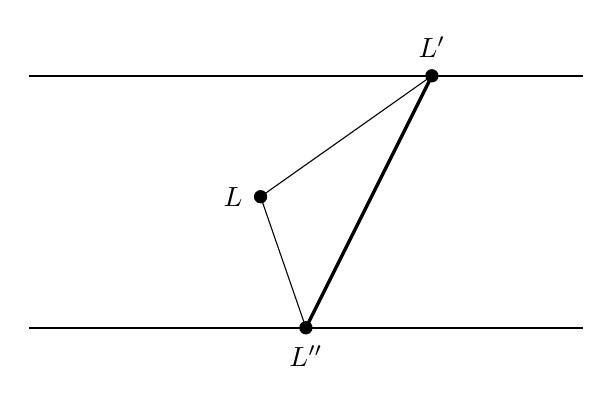
\begin{tikzpicture}[x=0.032cm,y=0.032cm]
  \draw[thick] (-20,100) -- (200,100);
  \draw[thick] (-20,0) -- (200,0);
  \draw[very thick] (90,0) -- (140,100);
  \draw (90,0) -- (72,52) -- (140,100);
  \foreach \x/\y in {90/0,140/100,72/52} { \fill (\x,\y) circle (2.4pt); }
  \node[below=3pt] at (90,0) {$L''$};
  \node[above=3pt] at (140,100) {$L'$};
  \node[left=3pt] at (72,52) {$L$};
\end{tikzpicture}
\caption{A characteristic leaf \label{fig:4.8}}
\end{figure}

\noindent
The vertices of the simplices forming the equilateral triangle
are given by
$\pi^{n_1}M_1 +\pi^{n_2}M_2 + M_3,\ 0 \leq n_2 \leq n_1 \leq b$.
The segment of length $|b|$ joining $L'$ to $L''$ is called the
{\bf characteristic base} or {\bf segment}. This base degenerates to a
vertex if $L \in \zz$ and otherwise it may be regarded as 
an equilateral triangle, under a suitable metric structure on $\bbg$.

\begin{lemma}
\label{lemma:4.9} 
(\cite{LaUn}) 
Suppose $g\in G(F)$ is such that $N_1(g)$
is elliptic regular. Then the following hold.

\begin{itemize}
\item[(a)] 
$g\sigma$ sends the characteristic leaf of $L$ to the characteristic leaf
of $g\check{L}$.

\item[(b)] 
For each vertex $\Lambda$ in $\bbH1$, $g\sigma$ sends the line 
$\{\pi^{-n}\off +\Lambda\ |\ n\in \zzz\}$
of $\zz$ with positive orientation to another line 
$\{\pi^m\off +\Lambda ' \ |\ m \in \zzz\}$ in
$\zz$ with reversed orientation.

\item[(c)] 
$g\sigma$ sends the characteristic base of the leaf for L to the
characteristic base (with orientation reversed) for $g\check{L}$;

\item[(d)] 
For any $h\in SL(2,F)$ representing $N_1(g)$, the action of
$h$ on $\zz$ is the same as the action of $(g\sigma)^2$ restricted
to $\zz$.
\end{itemize}
\end{lemma}

\begin{remark}
The $h \in H_1(F)$ in (d) is fixed for the rest of this section.
\end{remark}

\pf
We may assume by Corollary \ref{cor:1.14} that $g$ is represented by a 
$(2,1)$-block matrix $A\in GL(3,F)$ in the basis giving the embedding
$\zz$. From this the four statements (a)-(d) follow without difficulty
from simple facts about buildings. 
\qed

In particular, (d) implies that if $\overline{\Lambda '},
\ \overline{\Lambda ''}$ are lines associated to two fixed points
$\Lambda ', \Lambda ''$ of $h \in N_1(g)$ and if the endpoints $L'$, $L''$
of the vertices of the characteristic base lie on $\overline{\Lambda '},
\ \overline{\Lambda ''}$, respectively, then $g\sigma$ ``flips'' $L$
and its leaf about a certain ``dotted'' line $D_A$ (which depends only
on $A$, not on $L$, $L'$, $L''$, and lies in the first barycentric
subdivision of $\bbg$ but does not necessarily lie in $\bbg$):


%%figure (4.10) on page 1121
\begin{figure}[htbp]
\centering
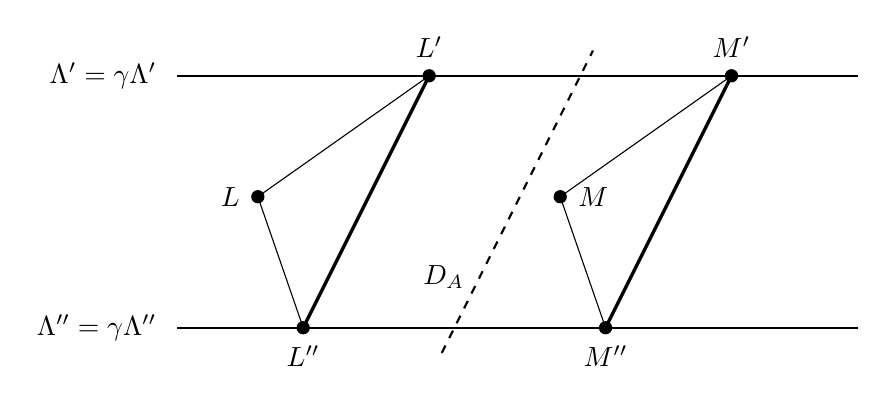
\begin{tikzpicture}[x=0.032cm,y=0.032cm]
  \draw[thick] (-60,100) -- (210,100);
  \draw[thick] (-60,0) -- (210,0);
  \node[left=4pt] at (-60,100) {$\Lambda'=\gamma\Lambda'$};
  \node[left=4pt] at (-60,0) {$\Lambda''=\gamma\Lambda''$};
  % left leaf
  \draw[very thick] (-10,0) -- (40,100);
  \draw (-10,0) -- (-28,52) -- (40,100);
  \foreach \x/\y in {-10/0,40/100,-28/52} { \fill (\x,\y) circle (2.4pt); }
  \node[below=3pt] at (-10,0) {$L''$};
  \node[above=3pt] at (40,100) {$L'$};
  \node[left=3pt] at (-28,52) {$L$};
  % right leaf
  \draw[very thick] (110,0) -- (160,100);
  \draw (110,0) -- (92,52) -- (160,100);
  \foreach \x/\y in {110/0,160/100,92/52} { \fill (\x,\y) circle (2.4pt); }
  \node[below=3pt] at (110,0) {$M''$};
  \node[above=3pt] at (160,100) {$M'$};
  \node[right=3pt] at (92,52) {$M$};
  % the line D_A
  \draw[thick,dashed] (45,-10) -- (105,110);
  \node[left=2pt] at (60,20) {$D_A$};
\end{tikzpicture}
\caption{Flipping characteristic leaves \label{fig:4.10}}
\end{figure}

\noindent
If $N_1(g)$ does not contain a unipotent then by Corollary 
\ref{cor:1.14} we may assume that the
matrix $A\in GL(3,F)\cong \text{Aut}_F(V_{A'}+W_{A'})$ 
representing $g=[A]$ is in block form:

\begin{equation}
\label{eqn:4.11}
A = 
\left(
\begin{array}{cc}
u\pi^c&\ \\\ &C
\end{array}
\right) ,
\ \ \ C\in GL(2,F),\ u\in \off^{\times},\ c\in\zzz . 
\end{equation}
(Here $[A']$ is the matrix in Corollary \ref{cor:1.14} 
which belongs to the same stable
$\sigma$--conjugacy class as $[A]$.)
In this case, $A\sigma$ sends the lattice $\pi^{-n}\off +\Lambda$ in $\zz$ to
$\pi^{c+n}\off +\Lambda '$, for some $\Lambda '$. If we parameterize
the vertices in the lines in Figure \ref{fig:4.8} 
by the integers then, in a sense, 
$D_A$ may be thought of 
as the ``$c/2$--line''. It belongs to $\bbg$ if and only if $c$ is even. 
Suppose that $c$ is even and that 

\begin{equation}
\label{eqn:4.12}
\begin{split}
&A\sigma : [\pi^{-n}\off +\Lambda] \longmapsto [\pi^{c+n}\off +\Lambda '],\\
&A\sigma : [\pi^{-n}\off +\Lambda '] \longmapsto [\pi^{c+n}\off +\Lambda].
\end{split}
\end{equation}
It can be shown without much effort that, in this case,  
$[\Lambda ],\ [\Lambda ']$ in $\zz$ correspond to two fixed points of
$h \in N_1(g)$ in $\bbH1$. Also, it is not hard to see that,

\begin{lemma}
\label{lemma:4.13}
%{Fact 4.13} 
Suppose c is even and L is a fixed point of
$[A]\sigma$ whose characteristic base has endpoints lying on the
lines $\overline{\Lambda '}\not= \overline{\Lambda ''}$. Then 
the following hold.

\begin{itemize}
\item[(a)] 
$D_A$ intersects the lines 
$\overline{\Lambda '},\ \overline{\Lambda ''}$
at the two vertices which determine the endpoints of the characteristic base 
of L and

\item[(b)] 
The lines $\overline{\Lambda '},\ \overline{\Lambda ''}$ in $\zz$
correspond to two fixed points of $h$ in $\bbH1$.
\end{itemize}
\end{lemma}

\begin{remark} 
There is a simpler version of this dealing with the case 
$\overline{\Lambda '}= \overline{\Lambda ''}$.
In this way, we will obtain a ``2-1'' correspondence, when
$c$ is even, between \underbar{pairs} of fixed points of $h$ in $\bbH1$ and
fixed points of $[A]\sigma$ in $\bbg$. One important point to bear in mind is 
that when $c$ is \underbar{odd} then the line $D_A$ cannot intersect $\bbg$
and therefore there can be \underbar{no} fixed points of $[A]\sigma$ in this
case. So far we have only shown that (when $c$ is even) given a fixed point 
of $[A]$ in $\bbg$ there are associated two fixed points
of $h$ in $\bbH1$.
\end{remark}
 
\begin{runex}[The action on $\mathcal Z$ and the line $D_A$]
\label{run:Zaction}
Write $\Lambda_{(n)}$ for the class of $3^n\mathbb Z_3e_0\oplus\Lambda$.
(In the indexing of the text this is the vertex $\pi^{-n}\off+\Lambda$
with $n$ replaced by $-n$.) Proposition~\ref{prop:new-Zfix}(a) gives,
for a lattice $\Lambda=M\mathbb Z_3^2$,
\begin{equation}\label{eq:run-Zaction}
 T_{A_a}\colon\ \Lambda_{(n)}\longmapsto (B\Lambda)_{(v_3(a)+v_3(\det M)-n)} .
\end{equation}
So $T_{A_a}$ covers the action of $B=Cw$ on the tree, and reverses
each line of $\mathcal Z$ that it preserves, as in
Lemma~\ref{lemma:4.9}(b). In all four specimens $B\Lambda_0=\Lambda_0$,
and the line over $[\Lambda_0]$ is mapped to itself by
$n\mapsto v_3(a)-n$. For $a=1$ the vertex $[L_0]$ is fixed, and for
$a=3$ the only fixed point of the line is the midpoint of the edge
joining $[L_0]$ and $[3\mathbb Z_3e_0\oplus\Lambda_0]$. This is the
statement that $D_A$ is the ``$c/2$-line'' on the line over
$[\Lambda_0]$.

The lines over the other vertices behave differently. In
specimen~III the matrix $B=1+3\smat{0}{-1}{1}{0}$ preserves each of the
four neighbors $p',p'',q_\pm$ of $[\Lambda_0]$ (as lattices, since
$B\Lambda\subseteq\Lambda+3\Lambda_0=\Lambda$), and for these
$v_3(\det M)=1$. On their lines \eqref{eq:run-Zaction} reads
$n\mapsto v_3(a)+1-n$. So $T_{A_1}$ fixes no vertex there, and
$T_{A_3}$ fixes the four vertices
\[
 [3\mathbb Z_3e_0\oplus\Lambda],\qquad
 [\Lambda]\in\{p',p'',q_+,q_-\}.
\]
The line $D_A$ therefore meets the lines of $\mathcal Z$ at heights
that alternate with the distance from $[\Lambda_0]$.
In specimen~II, $B$ fixes only $[\Lambda_0]$ and exchanges $p'$ with
$p''$ and $q_+$ with $q_-$; the corresponding lines of $\mathcal Z$
are flipped onto each other as in \eqref{eqn:4.12}.
\end{runex}

From the reduction of \S \ref{sec:3} 
one sees that it is also necessary to know what
happens when $A$ in (\ref{eqn:4.11}) is replaced by a matrix $A'$ 
stably $\sigma$--conjugate
to $A$ but not $\sigma$--conjugate to $A$ over $F$. Of course, 
$N_1([A])=N_1([A'])$ so $A'$ may be put in $(1,2)$-block 
form as in (\ref{eqn:4.11}),
for some $c'\in\zzz ,\ C'\in GL(2,F),\ u'\in\off^{\times}$. 
If moreover the eigenvalues of $h$ determine an unramified 
extension of $F$ then
$c'$ and $c$ have different parity. On the other hand, if $A'$ and $A$
are $\sigma$--conjugate over $F$ then $c$ and $c'$ do have the same parity, so
we have the following result.

\begin{lemma}
\label{lemma:4.14}
%{Fact 4.14} 
The parity of $c$ depends only on the rational
$\sigma$--conjugacy class of $[A]$. If the eigenvalues of $h$ determine an
unramified extension of $F$ (the ``unramified case'') and $A$, $A'$ are stably 
$\sigma$--conjugate but not
$\sigma$--conjugate over $F$ then either $c$ or $c'$ is even (but not both). 
\end{lemma}

By the previous paragraph, in this ``unramified case'', there is either 
a fixed point of $A\sigma$ (and $A'\sigma$ has no fixed point) or a
fixed point of $A'\sigma$ (and $A\sigma$ has no fixed point). 
 
\begin{draftremark}[The parity of $c$ requires a normalization]
\label{rem:c-parity}
The two matrices $\operatorname{diag}(\pi^c,C)$ and
$\operatorname{diag}(\pi^{c+1},\pi C)$ define the same element of
$PGL_3(F)$, so the parity of $c$ in \eqref{eqn:4.11} has a meaning
only after $C$ has been normalized. Running example~\ref{run:Zaction}
uses $C=-Bw$ with $\det B$ a unit. With that normalization, the line
over a tree vertex $[\Lambda]$ fixed by $B$ carries a fixed vertex of
$A\sigma$ exactly when $c\equiv t_2([\Lambda])\pmod2$
(Proposition~\ref{prop:new-Zfix}). When $|1+\beta_1|_E=1$ the matrix
$B$ fixes a single vertex and the dichotomy stated after
Lemma~\ref{lemma:4.14} holds in the running example (specimens I
and~II: counts $1,0$ and $5,0$). When $|1+\beta_1|_E<1$ it does not:
in specimen~III the two classes have $1$ and $4$ fixed vertices. The
statements of this subsection that are phrased in terms of the parity
of $c$ should be read with this in mind; a formulation valid for all
$m$ is among the obligations of Section~\ref{sec:new-todo}.
\end{draftremark}

The problem now is to deal with the converse of Lemma \ref{lemma:4.13}: 
given a pair of fixed points
of $h \in N_1(g)$, associate to them fixed point of $A\sigma$. Instead
of proving this, we shall prove that this holds ``on average'', which is
sufficient for our purposes.
For this the following lemma is crucial, but first we need some notation:
Let $d$ be the maximum distance
between two fixed points of $h$, let the eigenvalues of $h$
determine a quadratic extension $E$ of $F$, and suppose that

\begin{equation}
\label{eqn:4.15}
U(d):=U_d\pi^{2\zzz}:=
\{x\in\off^{\times}\ |\ x\equiv 1 \, {\rm mod}\, \pi^d\}\pi^{2\zzz}
\subseteq N_{_{E/F}}(E^{\times})
\end{equation}
is finite index in $F^{\times}$. Let ${\cal S}$ denote the set of 
$a\in F^{\times}$ for which
$P'\not= P''$ exist (for a fixed $p'$, $p''$) and satisfying (ai)-(aiv) in the 
lemma below. Here $A_a$ is defined to be a representative of $g_a$, where 
$g_a$ is defined in the paragraph following (\ref{eqn:3.16}) and $A$ is our
representative of $g$ chosen at the beginning of this section. We may,
by Corollary \ref{cor:1.14}, choose all the $A_a$ to be in block form as in 
(\ref{eqn:4.11}).
$A_a\sigma$ may have no
fixed points; however, if it does, let $P_0$ denote one of them. Let
$U_n$ denote the stabilizer of the action of 
$T_a :=(A_a\sigma )(A\sigma )^{-1}$ on $P_0$, for some $n\geq 0$, with
$U_n$ as in (\ref{eqn:4.15}).

\begin{lemma}
\label{lemma:4.16} 
(\cite{LaUn}, Lemma 5.1) 
Suppose that $p'$, $p''$ are 
vertices in
$\bbH1$ (possibly $p'$ = $p''$) and that $[A]\sigma$ ``flips'' the lines
in $\bbg$ associated to $p'$, $p''$ onto each other. Then:

\begin{itemize}
\item[(a)] 
For each $a\in F^{\times}$ there exists at most one pair $P'$, $P''$
of vertices in $\bbg$ with

\begin{itemize}
\item[(i)] 
$ P'$ lying on the line associated to $p'$,

\item[(ii)] 
$P''$ lying on the line associated to $p''$,

\item[(iii)]
In the notation of \S \ref{sec:3}, $A_a\sigma (P') = P'',
\ A_a\sigma (P'')=P'$.

\item[(iv)] 
$P'$, $P''$ form the extreme vertices of a characteristic
segment.
\end{itemize}

\item[(b)] 
Suppose $a\in F^{\times}$ is such that a pair $p'$, $p''$ exists for $A_a$.
Then a pair exists for $A_b$ (for the same $p'$, $p''$) if and only
if $aN_{_{E/F}}(E^{\times})=bN_{_{E/F}}(E^{\times})$.

\item[(c)] 
Let ${\cal S},\ P_0,$ and $U_n$ be as above, and assume that $n\geq 1$.
Then $n \leq d$ and there are $[\off^{\times}:U_n]$ distinct
P's with segment $(P',P'')$ such that $(A_a\sigma )P = P$.

\item[(d)] 
If $|{\rm Fix}(A_a\sigma )|\not= 0$ then $|{\rm Fix}(A_{a\pi}\sigma )|=0$,
for $E/F$ unramified.

\item[(e)] 
In the notation of part (c),

\[
{1\over{[\off^{\times}:U_d]}}\sum_{a\in F^{\times}/U(d)}
\sum_{\substack{ P\\A_a\sigma P = P\\P \text{ has segment }(P',P'')}}
1 
={1\over{[\off^{\times}:U_n]}}\sum_{a\in F^{\times}/U(n)}
\sum_{\substack{ P\\A_a\sigma P = P\\P \text{ has segment }(P',P'')}}
1 .
\]
\end{itemize}

There is an obvious ``$\kappa$--analog'' (see (\ref{eqn:3.18})) 
of the above equation 
whose statement is left to the reader.
\end{lemma}

\begin{remark} 
(a) When applying this lemma to (\ref{eqn:3.17}) or 
(\ref{eqn:3.18}), one uses the fact that

\[
{1\over{2}}[F^{\times}:U(n)] = [\off^{\times}:U_n].
\]
(b) For the situation in Lemma \ref{lemma:4.13}(c) when n = 0, 
see \S \ref{sec:5}. The ``matching''
is then $P = P' = P''\longmapsto p'=p''$.
\end{remark}

Let me now sketch the proof of this lemma. Consider the situation
described by the following diagram:

%%figure (4.17) on page 1123
\begin{figure}[htbp]
\centering
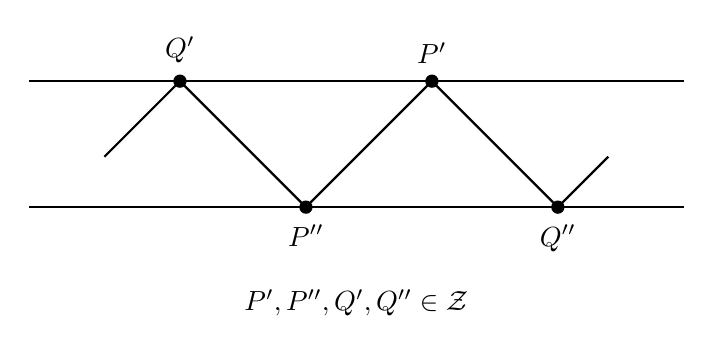
\begin{tikzpicture}[x=0.032cm,y=0.032cm]
  \draw[thick] (-60,50) -- (200,50);
  \draw[thick] (-60,0) -- (200,0);
  \draw[thick] (-30,20) -- (0,50) -- (50,0) -- (100,50) -- (150,0) -- (170,20);
  \foreach \x/\y in {0/50,50/0,100/50,150/0} { \fill (\x,\y) circle (2.4pt); }
  \node[above=3pt] at (0,50) {$Q'$};
  \node[above=3pt] at (100,50) {$P'$};
  \node[below=3pt] at (50,0) {$P''$};
  \node[below=3pt] at (150,0) {$Q''$};
  \node at (70,-38) {$P',P'',Q',Q''\in\mathcal Z$};
\end{tikzpicture}
\caption{Another band in the apartment \label{fig:4.17}}
\end{figure}

\noindent
In this case, as we've noted above, there are three rank one $\off$--modules
$M_1,\ M_2,\ M_3$ such that

\[
\begin{split}
&P' = [M_1+M_2+M_3],\ \ P''=[\pi^bM_1+\pi^bM_2 +M_3],\\
&Q' = [\pi^bM_1+M_2+M_3],\ \ Q''=[M_1+\pi^bM_2 +M_3].
\end{split}
\]

\begin{lemma}
\label{lemma:4.18}

\begin{itemize}
\item[(a)] 
The vertices $P$ in $\bbg$ with characteristic segment $(P',P'')$,
$P' \not= P''$, correspond to rank three lattices
$L+M_3$, where $L$ is a lattice satisfying
\newline
$\ \ (i) \pi^bM_1 +\pi^bM_2 \subseteq L \subseteq M_1+M_2,$
\newline
$\ \ (ii) \pi^{b-1}M_1 + \pi^{b-1}M_2 \not\subset L,$
\newline
$\ \ (iii) L \not\subset \pi M_1+\pi M_2,$
\newline
$\ \ (iv)  L \not\subset \pi M_1+ M_2 =:M',$
\newline
$\ \ (v) \  L \not\subset  M_1+\pi M_2=:M''.$
\newline

\item[(b)] 
If $u\in \off^{\times}$ then the action of 
$T_u := (A_u\sigma )(A\sigma )^{-1}$ on $\zz$ induces an action of 
$\off^{\times}$ on the lattices $L$ in (a). This action agrees with
that defined by the matrix

\[
\left(
\begin{array}{cc}
u&0\\0&1 
\end{array}
\right),
\]
and, moreover, it is transitive on the set of $L$'s.
\end{itemize}
\end{lemma}

\pf
(of Lemma \ref{lemma:4.18})
The stabilizer of any point $P$ with segment $(P',P'')$ under the action of 
$\off^{\times}$ via $T_u$ is of the form $U_b$, for some $b\geq 1$. Thus

\begin{equation}
\label{eqn:4.19}
P=A\sigma T_u(P)=T_uA\sigma (P)=A_u\sigma (P),
\end{equation}
for some $u\in\off$ uniquely determined modulo $U_b$. In other words, if $P$ 
has segment $(P',P'')$ then there is a $u\in \off^{\times}$ such that
$A\sigma T_u (P)=P$ and

\[
\left(
\begin{array}{cc}
u'&0\\0&1 \end{array}
\right),\ \ u'\in U_b,
\]
not only stabilizes $A\sigma (P)$ but also commutes with $T_u, \ u\in
\off^{\times}$. 
\qed

From these facts, Lemma \ref{lemma:4.16} follows. 
As a corollary, we obtain $r(0)=R(0)$,
using Lemma \ref{lemma:3.3} and (\ref{eqn:3.17}).

\begin{runex}[Characteristic leaves in specimen II]
\label{run:leaves}
In specimen~II, $h=1-3B$ is congruent to $1$ modulo $3$ and fixes the
five vertices $[\Lambda_0],p',p'',q_+,q_-$ of the tree, in agreement
with Lemma~\ref{lemma:4.5}: $\Delta(h)=3^{-1}$ and
$(3^2+3-2)/(3-1)=5$. On the twisted side, $[L_0]$ is the only fixed
vertex of $T_{A_1}$ in $\mathcal Z$ (Running example~\ref{run:Zaction}).
The other four fixed vertices of $T_{A_1}$ lie outside $\mathcal Z$:
\[
 L_\pm=\mathbb Z_3(e_0\pm e_2)+3\mathbb Z_3e_1+9\mathbb Z_3e_2,
 \qquad
 L'_\pm=\mathbb Z_3(e_0\pm e_1)+9\mathbb Z_3e_1+3\mathbb Z_3e_2 .
\]
Here is the verification for $L_+$. The basis
$f_1=e_0+e_2$, $f_2=3e_1$, $f_3=9e_2$ has dual basis
$e_0$, $\tfrac13e_1$, $\tfrac19(e_2-e_0)$. Since $Ce_1=-e_1$ and
$Ce_2=-3e_1-e_2$, the lattice $9A_1L_+^\vee$ is spanned by
$9e_0$, $3e_1$, and $e_0+3e_1+e_2$, that is, by $e_0+e_2$, $3e_1$,
and $9e_2$. So $A_1L_+^\vee=\tfrac19L_+$.

The characteristic segment of $L_+$ is visible from its intersection
with, and its projection to, the two summands:
\[
 P''=[(L_+\cap Fe_0)\oplus(L_+\cap W_A)]
    =[3\mathbb Z_3e_0\oplus(\mathbb Z_3e_1+3\mathbb Z_3e_2)],
 \qquad
 P'=[\mathbb Z_3e_0\oplus(3\mathbb Z_3e_1+\mathbb Z_3e_2)].
\]
These lie on the lines of $\mathcal Z$ over $p''$ and $p'$, the two
neighbors of $[\Lambda_0]$ exchanged by $B$, and
$T_{A_1}$ exchanges $P'$ and $P''$ by \eqref{eq:run-Zaction}. The
three vertices $P'$, $P''$, $[L_+]$ are pairwise at distance $2$:
the quotients of suitable representatives are
$(\mathbb Z/9)^2$, $\mathbb Z/9$, and $\mathbb Z/9$. They are the
corners of the equilateral triangle of Figure~\ref{fig:4.8} with
$b=2$, and the midpoint of the segment $P'P''$ is the fixed vertex $[L_0]$. The leaves $L_\pm$ share this segment, and the leaves
$L'_\pm$ have the segment with the roles of $p'$ and $p''$ exchanged.
The two leaves on one segment are exchanged by
$\operatorname{diag}(-1,1,1)$, which illustrates
Lemma~\ref{lemma:4.18}(b) with $[\off^\times:U_1]=2$.

The conjugate representative $A_2$ also has five fixed vertices, by
Lemma~\ref{lemma:4.4}. Its four leaves, found by enumeration, have
their segments over the other exchanged pair $q_+,q_-$. So the square
class of a unit $u$ for which $A_u$ has a leaf on a given segment
depends on the segment; compare Lemma~\ref{lemma:5.2}(b).

That the list of fixed vertices is complete was checked by
enumeration of the ball of radius $4$ about $[L_0]$. The total
$1+4=5$ equals $|\operatorname{Fix}(h)|$, as $R(0)=r(0)$ requires,
and $T_{A_3}$ has no fixed vertex.
\end{runex}

\subsection{The buildings for $PGL(3)$ and $PGL(2)$}
\label{sec:5}

Recall $H_1:=SL(2),\ H_2:=PGL(2),\ G:=PGL(3)$, and $N_1,\ N_2$
denote the Jacquet-Shalika norms (\ref{eqn:1.9}). 
We assume $p\not= 2$ without further mention.
 
Let $h \in N_1(g)\cap H_1(F)$ have eigenvalues $\beta_1,\
\beta_2=\beta_1^{-1}$ and
let $h'\in N_2(g)\cap H_2(F)$ be represented by a matrix $B\in GL(2,F)$
having eigenvalues $\lambda\beta_1,\ \lambda$, for some
$\lambda\in \overline{F}^{\times}$. 
Recall $\bbH1 = \bbh2$ and that the action
of $H_2(F)$ on $\bbh2$ is defined analogously to the action of $G(F)$
on $\bbg$. 
Let $E/F$ denote the extension of $F$ obtained by adjoining the
eigenvalues of $h$; we may assume $E/F$ 
is quadratic since the split case was
handled in \S \ref{sec:2}. 
Since the tree $\bbh2$ has no closed loops, one can easily
show that $h$ has fixed points only if 
$c\beta_i\in \oee^{\times}$, for some $c\in F^{\times}$.
 
Our strategy is
to prove, in the notation of \S \ref{sec:3}, that $s(0)=S(0)$ in the
following manner.

\begin{itemize}
\item[(a)] 
If $|1+\beta_1|_E=1$ then $r(0)=s(0)$, and the geometric argument
 establishes $|S(0)|=R(0)$. The signed equality also requires the
 transfer-factor normalization to be verified.

\item[(b)] 
If $E/F$ is ramified and $|1+\beta_1|<1$, the intended
conclusion is that the relevant building fixed-vertex counts vanish,
not that such eigenvalues are impossible. 

\item[(c)] 
If $|1+\beta_1|_E<1$ and $E/F$ is unramified, the geometric count
gives $|\operatorname{Fix}(h')|=1$ and hence $s(0)=Q$.
The corresponding twisted identity is $S(0)/Q=1$, or $S(0)=Q$. 

\end{itemize}
The ramified subcase in (b) is treated separately below.
The sign in \eqref{eqn:3.18} is prescribed by the Hilbert-symbol
normalization, not chosen independently for each orbital integral.
Proposition~\ref{prop:5.6} initially determines only $|S(0)|$;
identifying it with $s(0)$ requires a signed argument.

\begin{draftremark}[A ramified example]
\label{rem:ramified-example}
The ramified case described in (b) really exists. Take
$F=\mathbb Q_3$, $E=F(\sqrt3)$, and $\beta=2+\sqrt3$.
Then $\beta^{-1}=2-\sqrt3$, $N_{E/F}(\beta)=1$,
and $|1+\beta|_E<1$ although $E/F$ is ramified.
For example, $h=\left(\begin{smallmatrix}0&-1\\1&4\end{smallmatrix}\right)$
has these eigenvalues. The desired vanishing in this case is therefore
geometric, not a field-theoretic exclusion.
\end{draftremark}

\begin{lemma}
\label{lemma:5.1}
\begin{itemize}
\item[(a)] 
$s(0)\leq r(0)$.

\item[(b)] 
Assume that $|1+\beta_1|=1$. Then the number of
fixed points of $h$ is equal to the number of fixed points of $h'$,
i.e., $r(0)=s(0)$. Moreover, $|S(0)|\leq R(0)=r(0)$.
\end{itemize}
\end{lemma}

\pf
Part (a) follows immediately from Lemma \ref{lemma:3.3}. 
For part (b), recall $\Delta_{H_1}(h):=|1-\beta_1^2||\beta_1|^{-1}
=|1-\beta_1||1+\beta_1||\beta_1|^{-1}$ and
$\Delta_{H_2}(h'):=|1-\beta_1||\beta_1|^{-1/2}$, 
by the definitions in \S \ref{sec:2}.
The lemma now follows immediately from the counting 
formulas (\ref{eqn:3.17})-(\ref{eqn:3.18}) for
$R(0)$ and $S(0)$ and the hypothesis.
\qed

\begin{lemma}
\label{lemma:5.2}
\begin{itemize}
\item[(a)] 
The set {\rm Fix}($A_a\sigma$) is in one--to--one correspondence with the
L's such that

\[
[L] = [\{v\in V\ |\ {^{t}v}\cdot \, ^tA_a^{-1}\cdot v'\in \off ,
\ \forall v'\in L\}],
\]
i.e., the class of $L$ is self--dual with respect to the bilinear form of
$^tA_a^{-1}$.

\item[(b)] 
Assume $|{\rm Fix}(A\sigma )|\not= 0,\
[L]\in {\rm Fix}(A_u\sigma ),\ u\in \off^{\times},$
and $[L]\notin\zz$. Then $u=v^2$, for some $v\in\off^{\times}$, and in
particular $(u,\eps)_2=1$ (in the notation of (\ref{eqn:3.18})).
\end{itemize}
\end{lemma}

\pf
(a) This is a simple calculation using (\ref{eqn:4.3}): 
since $A\sigma$ sends $[L]$
to $[AL^{\vee}]$, $[L]$ is fixed if and only if $L$ belongs to the same
class as

\[
\begin{split}
AL^{\vee}
&=\{Av\in V\ |\ {^{t}v}\cdot v'\in \off ,
\ \forall v'\in L\}\\
&=\{v_o\in V\ |\  v_o=Av{\rm  and }\ {^{t}v}\cdot v'\in \off ,
\ \forall v'\in L\}.
\end{split}
\]
It is easy to see that this is equivalent to the statement in part (a).
\newline
(b) We may rephrase the problem in terms of self--dual lattice
classes. 
Let $P$ be an $^tA^{-1}$--self--dual lattice class. 
By (a) above and Lemma \ref{lemma:4.14},
the transitivity of $T_a$ implies that
there is an $a\in\off^{\times}$ such that $[L]=T_aP$. It follows that
$[L]$ is both
$^tA_u^{-1}$--self--dual and $^tA_{a^{-2}}^{-1}$--self--dual, since $T_a$ and
$A_b\sigma$ commute. 
This implies, by (a), that $[L]$ corresponds to a fixed
point of $T_{ua^2}$. 
However, by Lemma \ref{lemma:4.18} and the discussion following 
(\ref{eqn:4.15}), we know that the stabilizer of 
$T_{ua^2}$ is $U_n$,
where $n\geq 1$ is the distance between $[L]$ and its
projection $[L']$ in $\zz$ (by hypothesis, $[L]\not= [L']$).
Since, by definition,
$U_n \subseteq \{ {\rm squares\ in\ }\off^{\times}\}$, for $n\geq 1$, we
conclude that $u$ is a square in $\off^{\times}$.
\qed

\begin{lemma}
\label{lemma:5.3}
Let $w:=\left(\smallmatrix \ &1\\-1&\ \endsmallmatrix
\right)$, and let $\Lambda_0:=\off\oplus\off\oplus\off$ denote the standard
rank 3 lattice written in terms of a fixed basis for $V_A\oplus W_A$.
The action of $A_a\sigma$ on $\bbg$ is given on $\zz$ by

\[
\begin{split}
\left[ 
\left(
\begin{array}{cc} 
r&\ \\\ &C'
\end{array}\right)
\Lambda_0\right] \longmapsto
&\left[ A_a
\left(
\begin{array}{cc} 
1&\ \\ \ &w
\end{array}\right)
\left(
\begin{array}{cc} 
r^{-1}&\ \\
\ &C'
\end{array}\right)
\left(
\begin{array}{cc} 
1&\ \\\ &w
\end{array}\right)^{-1}\Lambda_0\right]\\
&=\left[ A_a
\left(
\begin{array}{cc} 
1&\ \\\ &w
\end{array}\right)
\left(
\begin{array}{cc} 
r^{-1}&\ \\\ &C'
\end{array}\right)
\Lambda_0\right],
\end{split}
\]
where $r\in F^{\times},\ C'\in {\rm Aut}_F(W_A)\cong GL(2,F)$.
\end{lemma}

\begin{remark} This follows from (\ref{eqn:4.3}) and the fact that
$C^{-1}=(det(C))^{-1}\, ^t(w^{-1}Cw)$. This description of the twisted
action on the building is especially useful when the action of
$A_a\sigma$ is restricted $\zz$.
\end{remark}

\begin{lemma}
\label{lemma:5.4} 
Assume that $N_1(g)$ doesn't contain any
unipotent element. If ${\rm Fix}(A\sigma )$
contains a
vertex \underbar{not} in $\zz$ and if
${\rm Fix}(A\sigma )\cap\zz = \emptyset$ then $|\beta'_1/\beta'_2 +1|<1$,
where $\beta'_i$ are the eigenvalues of $Cw$.
\end{lemma}

\pf 
By hypothesis, we may assume that A is of the form
$\left(\begin{array}{cc} 1 &\ \\ \ &C\end{array}\right)$, 
thanks to Corollary \ref{cor:1.14}.
Suppose that there is an $[L]\in {\rm Fix}(A\sigma )$ not in $\zz$. 
Lemma \ref{lemma:4.16}
implies that we can find $[L'],\ [L'']\in\zz$ forming the characteristic
segment of $[L]$ such that
$[A\sigma L'] = [L''],\ [A\sigma L''] = [L']$. 

Denote by $p',\ p''$
the vertices of $\bbb (SL(2))$ associated to $L',\ L''$,
where $Aw(p')=p'',\ Aw(p'')=p'$.
These are depicted by the lines in Figure \ref{fig:4.8}.
%%%%%%%%%%Last sentence added 3-2003 to avoid redrawing 4.8 
We may consider the midpoint $p_0$ of $p',\ p''$ in the first barycentric
subdivision of $\bbb (SL(2,F))$ as a vertex of the tree over $E$, since
$E/F$ is ramified. By Lemma \ref{lemma:5.3} and a
well--known result on trees, $p_0$ in $\bbb (SL(2,E))$ is a fixed point
of $Cw$ ($Cw$ acts without inversion on the first barycentric subdivision
of $\bbb (SL(2,F))$). By Lemma \ref{lemma:5.3}, this midpoint
is associated to a fixed point $[L_0]$ over E of ($A\sigma$ and)
$A\cdot\left(\begin{array}{cc}
1&\ \\\ &w\end{array}\right)$. By hypothesis 
$[L_0]\notin \zz$.
 
Let
$p_1,\ p_2$ be two neighbors of $p_0$, with $p_i$ a vertex in
$\bbb (SL(2,F))$ and with $Cw(p_1)=p_2,\ Cw(p_2)=p_1$. There is an
apartment containing $p_1,\ p_2$ in which we can write

\begin{equation}
\begin{split}
&p_1 = [\pi^{b_1+1}e_1\off + \pi^{b_2}e_2\off ],\\
&p_2 = [\pi^{b_1}e_1\off + \pi^{b_2}e_2\off ],
\end{split}
\label{eqn:5.5}
\end{equation}
for some $b_i\in\zzz$ and a suitable basis $\{e_1,\ e_2\}$. It follows that
$Cw$ is conjugate over $F$ to
$\left(\smallmatrix u_1\pi^{-1}&u_2\pi^{b_1-b_2}\\ u_3\pi^{b_2-b_1-1}&
u_4\endsmallmatrix\right)$,
for some $u_i\in \off^{\times}$. After multiplying the matrix by a
scalar in $F^\times$, this is projectively conjugate over $F$ to
\[
\begin{pmatrix}
u_1\pi^{b_1-b_2} &u_2\pi^{2(b_1-b_2)+1}\\
u_3&u_4\pi^{b_1-b_2+1}
\end{pmatrix}.
\]
If $b_1-b_2\leq -2$ or
$b_1-b_2\geq 1$ then the quotient of the eigenvalues
of this matrix are equal to $-1 \pm \epsilon$, for some
$|\epsilon |<1$. 
In this case, from Lemma \ref{lemma:4.5} we find that
$Cw$ can have at most one fixed point in the tree over $E$,
and none in the tree over $F$. In this case,
we conclude that
there is no fixed point of $A\sigma$ in $\zz$. The cases $b_1-b_2=-1$
and $b_1-b_2=0$ are similar: if $b_1-b_2=-1$ then $p_1=[\Lambda_0]$
and $p_2=[\pi^{-1}e_1\off +\Lambda_0]$. It follows that
$Cw$ is conjugate over $F$ to
$\left(\smallmatrix u_1&u_2\pi^{-1}\\ u_3&u_4\endsmallmatrix\right)$,
for some $u_i\in \off^{\times}$, and the same conclusion may be drawn.
The case $b_1-b_2=0$ is similar and therefore omitted.  
\qed

\begin{proposition}
\label{prop:5.6}
If $|1+\beta_1|_E = 1$ then $|S(0)| = s(0)$.
\end{proposition}

\pf 
Again, by hypothesis, we may assume that $A$ is of the form
$\left(\begin{array}{cc}
1&\ \\\ &C\end{array}\right)$, thanks to Corollary
\ref{cor:1.14}.
 
Note that by the reduction formulas and Lemma \ref{lemma:5.2}(b), we have

\begin{equation}
R(0) - |S(0)| \leq 2Q(|{\rm Fix}(A\sigma )\cap \zz |
+|{\rm Fix}(A_a\sigma )\cap \zz |),
\label{eqn:5.7}
\end{equation}
where $A$ and $A_a$ represent $\ddd_\sigma (g)$ (see (\ref{eqn:1.25})). 
Thus if ${\rm Fix}(A\sigma )\cap\zz = \emptyset$ were true, 
Lemma \ref{lemma:5.1}
would imply the result. Moreover, since
$|S(0)| \leq R(0) = r(0) = s(0)$, we may immediately dispose of the
case $R(0) = 0$. We may therefore assume that $\Delta (h) < 1$, so that
$|1-\beta_1|<1$ and that $|{\rm Fix}(A\sigma )|>0$.
 
Suppose for the moment that ${\rm Fix}(A\sigma ) \subset \zz$.
By Lemma \ref{lemma:4.16}(b) 
it follows that ${\rm Fix}(A_a\sigma ) =\emptyset $,
so we have $S(0) = R(0)$.
 
Suppose next that ${\rm Fix}(A\sigma )$ is not a subset of $\zz$. Since
${\rm Fix}(A_a\sigma ) \subset \zz$ 
would contradict Lemma \ref{lemma:4.16},
we must then have that ${\rm Fix}(A_a\sigma )$ is not a subset
of $\zz$. 
From Lemma \ref{lemma:4.16} 
we have that ${\rm Fix}(A\sigma ) \cap \zz \not= \emptyset$
or ${\rm Fix}(A_a\sigma ) \cap \zz \not= \emptyset$. Suppose without loss of 
generality that 
${\rm Fix}(A\sigma ) \cap \zz \not= \emptyset$. 
By (\ref{eqn:1.25}) and 
Lemma \ref{lemma:4.16}(b), if $E/F$ was 
ramified then we may take $a\in \off^{\times}$
(since $F^{\times}/N(E^{\times})$ is represented by a unit in the
case of a ramified extension $E/F$).
In this case, Lemma \ref{lemma:5.2}(b) implies all the signs in 
(\ref{eqn:3.18}) are
the same, so $|S(0)|=R(0)$. On the other hand, if $E/F$ were
unramified then $a\notin \off^{\times}$ by 
Lemma \ref{lemma:4.14} and then
Lemma \ref{lemma:4.16}(d) forces ${\rm Fix}(A_a\sigma ) \cap \zz = \emptyset$.
Then Lemma \ref{lemma:5.4} implies that $Cw$ has no fixed points, which
by Lemma \ref{lemma:5.3} would contradict our assumption.
\qed

Next we must consider the case where $|1+\beta_1|<1$ and $E/F$ is unramified.
In this case, $\Delta (h') = 1$, so by the formula for the number of fixed
points we have $|{\rm Fix}(h')| = 1$. On the other hand, the same formula
implies that $|{\rm Fix}(h)| > 1$, so it is clear that in this case
$r(0) > s(0)$. We of course want to show that the normalized signed sum in the
formula for $S(0)/Q$ is equal to $1$, so $s(0)=Q$. We want to show that,
if $|1+\beta_1| = q^{-m}$ with $m>0$ and $|{\rm Fix}(A\sigma )|\not= 0$
then

\begin{equation}
\begin{aligned}
\frac{S(0)}{Q}
&=\frac{\pm2}{[F^\times:U]}|(1+\beta_1)(1+\beta_2)|^{1/2}
\\[-2pt]
&\quad\cdot
\sum_{a\in F^\times/U}
\sum_{\substack{P\\\operatorname{Inv}(A_a\sigma(P),P)=0}}
\kappa(A_a)=1.
\end{aligned}
\label{eqn:5.10}
\end{equation}
In other words, we want to show that

\begin{equation}
{2\over{[F^{\times}:U]}}
\sum_{\substack{ a\in F^{\times}/U\\ (a,\epsilon)_2 =+1}}
\sum_{\substack{ P\\ {\rm Inv}(A_a\sigma (P),P) = 0}} 1
= q^m + {2\over{[F^{\times}:U]}}
\sum_{\substack{ a\in F^{\times}/U\\ (a,\epsilon)_2=-1}}
\sum_{\substack{ P\\ {\rm Inv}(A_a\sigma (P),P) = 0}} 1\ .
\label{eqn:5.11}
\end{equation}
For this it clearly suffices to prove that
\begin{equation}
{2\over{[F^{\times}:U]}}
\sum_{\substack{ a\in F^{\times}/U\\ (a,\epsilon)_2 =+1 }}
\sum_{\substack{ P\\ {\rm Inv}(A_a\sigma (P),P) = 0 }} 1
={{q^{m+1}+q^m-2}\over{q-1}}+R,
\label{eqn:5.12}
\end{equation}
(the ``unramified case''), and

\begin{equation}
{2\over{[F^{\times}:U]}}
\sum_{\substack{ a\in F^{\times}/U\\ (a,\epsilon)_2 =-1 }}
\sum_{\substack{ P\\ {\rm Inv}(A_a\sigma (P),P) = 0 }} 1
={{2(q^m - 1)}\over{q-1}}+R,
\label{eqn:5.13}
\end{equation}
(the ``ramified case'') for some $R$. 
These are due to the fact that every fixed point $P$ of $A$ gives
rise to a characteristic leaf by Lemma \ref{lemma:4.16}, 
hence to a fixed point in the
first barycentric subdivision of ${\cal B}(SL(2,F))$. The difference
of (\ref{eqn:5.12}) and (\ref{eqn:5.13}) 
merely counts the difference between the
sets of fixed points in the 
first barycentric subdivision of ${\cal B}(SL(2,F))$ in the unramified case
and in the ramified case, respectively. 
The number of such fixed 
points is as stated in (\ref{eqn:5.12}) by 
Lemma \ref{lemma:4.5}(a), in the unramified
case, and by Lemma \ref{lemma:4.5}(b) in the ramified case.
 
It remains to dispose of the case $|1+\beta_1|<1$ and $E/F$ ramified.
Although one must be able to deal with this case by a more direct argument,
I will give the following geometric proof. 
Since $|1-\beta_1|=1$ and $E/F$ is ramified, 
it follows from \cite{La80b}, p. 50,
for example, that $h'$ has no fixed points. 
This implies that $s(0)=0$ and
(by the proof of Lemma \ref{lemma:5.4}) that
$A\sigma$ has no fixed points in $\zz$. 
Thus each fixed point of $A\sigma$, which we may 
assume exists, is associated to a
characteristic base which is not a vertex.
By the remarks preceding Figure \ref{fig:4.10}, the fact that
$A\sigma$ has no fixed points in $\zz$ implies
that, in the notation of (\ref{eqn:5.7}),
$A_a\sigma$ will have fixed points in $\zz$ (since $E/F$ is ramified,
there is an element of valuation one in $N_{E/F}(E^\times )$
and therefore we may take $A_a$ to correspond to this element; the midpoint
of the characteristic base isn't a vertex,
whereas the midpoint of the dotted line $D_{A_a}$ associated to the fixed
point $L$ of $A\sigma$ in Figure \ref{fig:4.10} is a vertex in $\zz$
since the valuation of $a$ is one). By Lemma \ref{lemma:5.3}, 
this implies that,
in the notation of the proof of Proposition \ref{prop:5.6},
$Cw$ has fixed points. By Lemma \ref{lemma:5.3},
this contradicts the fact that $A\sigma$ has no fixed points in $\zz$.
 
For the unramified case with $|1+\beta_1|_E<1$,
\eqref{eqn:5.12} and \eqref{eqn:5.13} give a difference of $q^m$;
since $|(1+\beta_1)(1+\beta_2)|^{1/2}=q^{-m}$,
\eqref{eqn:5.10} yields $S(0)/Q=1$, hence $S(0)=Q=s(0)$.
The ramified vanishing argument above uses Lemmas~\ref{lemma:5.3}
and \ref{lemma:5.4}. The signed equality when
$|1+\beta_1|_E=1$ also depends on the signed transfer-factor
normalization, as distinguished from the absolute-value statement of
Proposition~\ref{prop:5.6}.

\begin{runex}[The cases (a), (b), (c) over $\mathbb Q_3$]
\label{run:case-split}
The four specimens fall under the three cases of the strategy at the
start of this subsection. Write $n_a=|\operatorname{Fix}(T_{A_a})|$,
and use \eqref{eqn:3.18} with $U=N_{E/F}(E^\times)$, so that
$S(0)=\pm|(1+\beta_1)(1+\beta_2)|^{1/2}\,Q\sum_a\kappa(A_a)\,n_a$ with
$Q=52/27$. The values of $\kappa$ are those of
Running example~\ref{run:kappa}.

\emph{Case (a): specimens I and II.} Here $|1+\beta_1|_E=1$. In
specimen~I, $h$ and $h'$ each fix only $[\Lambda_0]$ (both have
irreducible characteristic polynomial modulo $3$), and
$(n_1,n_3)=(1,0)$. The proof that $n_1=1$ is direct:
$T_{A_1}^2$ acts by $\gamma=\operatorname{diag}(1,h)$, whose
eigenvalues $1,\pm\sqrt{-1}$ are distinct modulo $3$. Since
$\det\gamma=1$, a lattice whose class is fixed by $\gamma$ is itself
preserved, so it is a module over
$\mathbb Z_3[\gamma]\simeq\mathbb Z_3\times\mathbb Z_3[\sqrt{-1}]$, so
it is $3^n\mathbb Z_3e_0\oplus3^j\Lambda_0$; the fixed vertices of
$\gamma$ are exactly the line over $[\Lambda_0]$, on which $T_{A_a}$
acts by $n\mapsto v_3(a)-n$. Hence $\sum_a\kappa(A_a)n_a=1$ and
$|S(0)|=Q=s(0)$. In specimen~II, $(n_1,n_3)=(5,0)$ by
Running example~\ref{run:leaves}, the element $h'\equiv2$ modulo $3$
fixes the same five tree vertices as $h$, and
$|S(0)|=5Q=R(0)=r(0)=s(0)$. In both specimens only one of the two
classes has fixed vertices, as in the proof of
Proposition~\ref{prop:5.6}.

\emph{Case (c): specimen III.} Here $|1+\beta_1|_E=3^{-1}$, so $m=1$.
The element $h$ fixes five tree vertices and $h'$, which is
$\smat{0}{1}{-1}{0}$ modulo $3$ up to a unit, fixes only
$[\Lambda_0]$; so $r(0)=5Q$ and $s(0)=Q$. On the twisted side
$(n_1,n_3)=(1,4)$, all in $\mathcal Z$
(Running example~\ref{run:Zaction}; that there are no leaves was
checked by enumeration and agrees with $R(0)=r(0)$). So
\[
 R(0)=Q(1+4)=5Q,\qquad
 \sum_a\kappa(A_a)\,n_a=4-1=3=q^m,\qquad
 S(0)=\pm3^{-1}\cdot Q\cdot3=\pm Q .
\]
The two counts are $4=(q^{m+1}-1)/(q-1)$ and $1=(q^m-1)/(q-1)$. In the
notation of \eqref{eqn:5.12} and \eqref{eqn:5.13} they are
$B_v(1)+R$ and $B_e(1)+R$ with $R=-1$; see
Proposition~\ref{prop:new-parity} for the general pattern.

\emph{Case (b): specimen IV.} Here $E=\mathbb Q_3(\sqrt3)$ is
ramified and $|1+\beta_1|_E<1$. The matrix $h'=\smat{3}{3}{1}{3}$ has
determinant $6$, of odd valuation, so it fixes no vertex of the tree
(Proposition~\ref{prop:new-tree-parity}) and $s(0)=0$. The element
$h=2+\smat{0}{3}{1}{0}$ generates the maximal order of $E$, so the
lattices it preserves are the fractional ideals of $E$; it fixes the
two ends $[\Lambda_0]$ and $p'$ of one edge. On the twisted side
$n_1=n_2=1$: the fixed vertex is $[L_0]$ in both classes. So
$\sum_a\kappa(A_a)n_a=1-1=0$ and $S(0)=0=s(0)$. The vanishing is a
cancellation between the two rational classes, not an absence of
fixed vertices.
\end{runex}

\begin{draftremark}[What the running example says about the sign]
\label{rem:sign-evidence}
With $\kappa$ computed from its definition \eqref{eqn:1.25}, as in
Running example~\ref{run:kappa}, the signed sums
$\sum_a\kappa(A_a)n_a$ of the four specimens are $1$, $5$, $3$, $0$,
all nonnegative, and $|(1+\beta_1)(1+\beta_2)|^{1/2}\,Q$ times them is
$s(0)$ in each case. If instead the sign is assigned by the rule
$\pm\kappa(g_a)=(a,\epsilon)_2$ of \eqref{eqn:3.18} with the labeling
$g_a\leftrightarrow A_a$ and one fixed choice of $\pm$, the sums are
$1$, $5$, $-3$, $0$. The two rules differ by the factor
$\kappa(A_1)$, which is $-1$ in specimen~III. This is numerical
evidence, in four cases over $\mathbb Q_3$, that the signed identity
$S(0)=s(0)$ holds when $\kappa$ is defined by \eqref{eqn:1.25}, and
that the initial $\pm$ of \eqref{eqn:3.18} depends on the base point
of the labeling. It is not a proof, and the representatives $g_a$ of
Section~\ref{sec:3} are not defined there explicitly enough to decide
whether they agree with the $A_a$ used here.
\end{draftremark}

\begin{draftremark}[Remaining verification]
The following steps are dependencies of a complete independent proof:
(i) verify the sign of $S(0)$ with the fixed convention in
\eqref{eqn:3.18} when $|1+\beta_1|_E=1$;
(ii) supply the omitted boundary valuation calculation in
Lemma~\ref{lemma:5.4} for $b_1-b_2=-1,0$;
(iii) verify the fixed-point comparison underlying the last ramified
vanishing argument; and (iv) verify the class-invariant averaging
in the precise geometric parametrization used in Section~\ref{sec:4}.
Until these checks are supplied, this corrected draft should not be
read as an independent certification of every step of the final
fundamental-lemma comparison.
\end{draftremark}

 

\section{The identities in the split case}
\label{sec:2}

\subsection{Summary}

The object is to briefly sketch, following \cite{LaUn}, a proof of the stable
and unstable fundamental lemmas

\begin{equation}
\label{eqn:2.1}
\Phi^{T,1}(g,\phi ) = \Phi^{T_1,1}(h,f),
\end{equation}
for $h\in N_1(g)\cap A_1(F)$ regular semi--simple, and

\begin{equation}
\label{eqn:2.2}
\Phi^{T,\kappa}(g,\phi ) = |(1+\beta_1)(1+\beta_2)|^{-1/2}\Phi(h',f),
\end{equation}
for $h'\in N_2(g)\cap A_2(F)$ regular, semi--simple. Here $A_i(F)$ denotes
the maximal split torus in $H_i(F)$; let $A(F)$ denote the maximal split torus
of G(F). The norms have been defined in such a way that, if $g\in A(F)$
then $N_i(g)\cap A_i(F) \not= \emptyset$. We use Satake transforms,
a method which has the advantage of yielding, for the split groups
we consider, an explicit expression for the absolute value of the
transfer factor (the precise transfer factor is very difficult to predict in
general, see the recent work of R. Langlands and D. Shelstad \cite{LS87}).

\subsection{Background on twisted integration formulas}
\label{sec:2.2}

All Haar measures in this subsection are normalized as in \cite{Ca79}.
\par
In this section, let $G' =SL(n)$ or $PGL(n)$ 
and consider the outer automorphism
$\sigma (g) = J'\cdot {^{t}g}^{-1}\cdot J'$ where $J'$ denotes the $n\times n$
skew--diagonal matrix with alternating $\pm 1's$ on the skew--diagonal:

\[
J':=
\left(
\begin{array}{cccccc}
 \ &\ &\ &\ &\ &1\\
\ &\ &\ &\ &-1&\ \\
\ &\ &\ &.&\ &\ \\
\ &\ &.&\ &\ &\ \\
\ &.&\ &\ &\ &\ \\
(-1)^{n-1}&\ &\ &\ &\ &\
\end{array}
\right) .
\]
Let $Ad$ denote the action of $G'(F)$ on Lie$(G')$:
$Ad(g)X :=gXg^{-1}$. 
The differentials at the identity of the maps
$n\mapsto nmn^{-1}m^{-1}$ and $n\mapsto
nm\sigma(n)^{-1}m^{-1}$ are respectively
$1-\operatorname{Ad}(m)$ and $1-\operatorname{Ad}(m)\sigma$.
The corresponding Jacobian factors are
$\Delta(m):=|\det(\operatorname{Ad}(m)-1)_{\operatorname{Lie}N'}|_F$
and $\Delta_\sigma(m):=
|\det(\operatorname{Ad}(m)\sigma-1)_{\operatorname{Lie}N'}|_F$.
These are \emph{linearizations}, not exact exponential identities for
nonabelian $N'$. In root-height coordinates, the maps are triangular,
with the indicated linear maps on the successive graded pieces. Where
these graded maps are invertible, their determinant gives the
change-of-variables modulus used below.
 
To be concrete, if $\alpha_1,\dots,\alpha_n$ are the simple roots of $G'$ then
$\sigma$ acts on their associated root groups via
$\sigma (\exp (tX_{\alpha_i})) = J(\exp (tX_{\alpha_i}))^{-1}J
= (-1)^{n-1}\exp (-tJ{^{t}X}_{\alpha_i}J)$,
or equivalently, via the action of $\sigma \in Out(G')\cong
{\rm Aut}(\ddd )$ on the Dynkin diagram $\ddd $ of $G'$. 
For $PGL(3)$, $\sigma$ exchanges the two simple roots; on the level of the
Lie algebra, it exchanges the root vectors $X_{\alpha_1},
\ X_{\alpha_2}$ and changes the sign of $X_{\alpha_1+\alpha_2}$
in Lie$\,N'$ since $X_{\alpha_1+\alpha_2}=[X_{\alpha_1},X_{\alpha_2}]$.
Therefore the analog to

\begin{equation}
\label{eqn:2.3}
\int_{N'} \phi (nmn^{-1}m^{-1})\ dn
= \Delta (m)^{-1}\int_{N'} \phi (n)\ dn 
\end{equation}
becomes

\begin{equation}
\label{eqn:2.4}
\int_{N'} \phi (nm\sigma (n)^{-1}m^{-1})\ dn
= \Delta_{\sigma}(m)^{-1}\int_{N'} \phi (n)\ dn 
\end{equation}
 
Let $a\in A'(F)$
belong to the maximal split torus of $G'(F)$ and let $\phi$ be a spherical
function on $G'(F)$. As a straightforward application of 
(\ref{eqn:2.3})-(\ref{eqn:2.4}), we
have

\begin{equation}
\label{eqn:2.5}
\begin{split}
\int_{G'(g\sigma ,F)\setminus G'(F)}
&\phi (x^{-1}g\sigma (x))\ d\ovx\\
&=\int_{G'(g\sigma ,F)\setminus A'(F)}\Delta_{\sigma}(m)^{-1}\Delta (m)
\int_{A'(F)\setminus G'(F)} \phi (x^{-1}mx)\ d\ovx d\ovt ,
\end{split}
\end{equation}
where $m:=t^{-1}a\sigma (t)$. Notice that the outer integral on the
right is a finite sum. This fact will be used in a later subsection.
 
The remainder of this subsection is devoted to the calculation of the
twisted Jacobian $\Delta_{\sigma}(m)$, when $G' = G = PGL(3)$. Write
Lie$\,N = F\cdot X_{\alpha_1}\oplus F\cdot X_{\alpha_2}
\oplus F\cdot X_{\alpha_1+\alpha_2}$ and identify its elements as
column vectors. In terms of this basis, $\sigma$ is represented by
the matrix

\[
\left( 
\begin{array}{ccc} 
\ &-1&\ \\
-1&\ &\ \\
\ &\ &-1
\end{array} 
\right)
\]
and $Ad(a)$ is represented by the matrix

\[
\left( 
\begin{array}{ccc} 
\alpha_1(a)&\ &\ \\
\ &\alpha_2(a)&\ \\
\ &\ &(\alpha_1+\alpha_2)(a)
\end{array} 
\right),
\]
where of course $\alpha_1(a) = a_1/a_2,\ \alpha_2(a) = a_2/a_3,
\ (\alpha_1 +\alpha_2)(a) = a_1/a_3$. Combining this together, we find
that ${\rm det} (Ad(a)\sigma -1)_{Lie\, N}= (a_1/a_3)^2-1$.
In particular, with $a = m = t^{-1}g\sigma (t) \left( \smallmatrix
\gamma_1t_1^{-1}t_3^{-1}&\ &\ \\
\ &\gamma_2t_2^{-2}&\ \\
\ &\ &\gamma_3t_1^{-1}t_3^{-1}\endsmallmatrix\right)$,
where $\gamma_i$ denote the eigenvalues of a representative of $g\in A(F)$,
we find that

\begin{equation}
\label{eqn:2.6}
\Delta_{\sigma}(m) = |1-(\gamma_1/\gamma_3)^2|_F.
\end{equation}

\subsection{The Satake transform on $PGL(3)$, $SL(2)$, $PGL(2)$}
\label{sec:2.3}

There are, as we mentioned already in \S \ref{sec:1}, $L$--maps

\[
\begin{split}
&\lambda_1:{^{L}H_1}(\ccc ) \rightarrow {^{L}G}(\ccc ),
\ \ \ {^{L}H_1} = SO(3)\\
&\lambda_2:{^{L}H_2}(\ccc ) \rightarrow {^{L}G}(\ccc ),
\ \ \ {^{L}H_2} = SL(2),
\end{split}
\]
given on the maximal split torus by

\[
\begin{split}
&\lambda_1 : 
\left( 
\begin{array}{cc} 
t_1&\ \\ 
\ &t_2
\end{array} 
\right) 
\longmapsto
\left( 
\begin{array}{ccc} 
t_1t_2^{-1}&\ &\ \\
\ &1&\ \\
\ &\ &t_2t_1^{-1}
\end{array} 
\right) ,\\
&\lambda_2 : 
\left( 
\begin{array}{ccc} 
t&\ \\ \ &t^{-1}
\end{array} 
\right) \longmapsto
\left( 
\begin{array}{ccc} 
t&\ &\ \\
\ &t^{-1}&\ \\
\ &\ &1
\end{array} 
\right) .
\end{split}
\]
Define the {\bf Satake transform} by

\begin{equation}
\label{eqn:2.7}
\begin{split}
&\hat{\phi}(t) := \sum_{\Lambda \in X^*({^{L}A})} \alpha (\Lambda )\Lambda (t),
\ \ t\in {^{L}A}(\ccc ),\\
&\hat{f_1}(t) := \sum_{\mu \in X^*({^{L}A_1})} \beta_1(\mu )\mu (t),
\ \ t\in {^{L}A_1}(\ccc ),\\
&\hat{f_2}(t) := \sum_{\nu \in X^*({^{L}A_2})} \beta_2(\nu )\nu (t),
\ \ t\in {^{L}A_2}(\ccc ).
\end{split}
\end{equation}
Here

\begin{equation}
\label{eqn:2.8}
\alpha (\Lambda ):=\Delta_G (g)\int_{A(F)\setminus G(F)}
\phi (x^{-1}gx)\ d\ovx ,
\end{equation}
where $\Lambda$ is that element $\Lambda =\Lambda (g)
=\Lambda (k_1,k_2,k_3) \in X^*({^{L}A})
\cong \zzz^3$ is that element corresponding to $(k_1,k_2,k_3)\in \zzz^3$
for $k_i$ given by

\[
g = \left( \begin{array}{ccc} u_1\pi^{k_1}&\ &\ \\
\ &u_2\pi^{k_2}&\ \\
\ &\ &u_3\pi^{k_3}\end{array} \right) ,\ \ u_i\in \off^{\times}.
\]
We also define $\Delta_G(g)
:=\prod_{{\rm all\  roots }\alpha }|1-\alpha (g)|^{1/2}
=\prod_{1\leq i<j\leq 3}
\left|\left(1-\frac{\gamma_i}{\gamma_j}\right)
\left(1-\frac{\gamma_j}{\gamma_i}\right)\right|_F^{1/2}.$ Similarly, for $H_1(F)$ we have

\begin{equation}
\label{eqn:2.9}
\eta_1 (\mu ):=\Delta_{H_1} (h)\int_{A_1(F)\setminus H_1(F)}
f_1(x^{-1}hx)\ d\ovx ,
\end{equation}
where $\mu =\mu (h)= \mu (m) \in X^*({^{L}H_1})\cong \zzz$ corresponds to

\[
h = \left( \begin{array}{cc} \beta_1&\ \\ \ &\beta_2
\end{array}
\right)
= \left( 
\begin{array}{cc}
u'_1\pi^{m}&\ \\ 
\ &u'_2\pi^{-m}
\end{array}
\right),
\]
where $u'_i\in \off^{\times}$.
Here we define $\Delta_{H_1}(h)
:=\prod_{{\rm all\  roots }\alpha }|1-\alpha (h)|^{1/2}
=|1-\beta_1/\beta_2||\beta_2/\beta_1|^{1/2}.$
For $H_2(F)$ we define $\Delta_{H_2}(h')
:=\prod_{{\rm all\  roots }\alpha }|1-\alpha (h')|^{1/2}
=|1-\beta '_1||\beta '_1|^{-1/2}$, and

\begin{equation}
\label{eqn:2.10}
\eta_2 (\nu ):=\Delta_{H_2} (h')\int_{A_2(F)\setminus H_2(F)}
f_2(x^{-1}h'x)\ d\ovx ,
\end{equation}
where $\nu = \nu (n_1,n_2) \in X^*({^{L}H_2})$ corresponds to

\[
h' = \left( 
\begin{array}{cc}
\lambda\beta '_1&\ \\ \ &\lambda
\end{array}
\right)
= \left( 
\begin{array}{cc}
u''_1\pi^{n_1}&\ \\ \ &u''_2\pi^{n_2}
\end{array}
\right) ,
\]
where
$u''_i \in \off^{\times}$. Here the pair
$(n_1,n_2) \in\zzz^2$ is not well--defined but $n_1 -n_2$ is.
 
Note that, via the induced map
$\lambda_1^* : X^*({^{L}A})\rightarrow X^*({^{L}A_1}),$
two $\Lambda (k_1,k_2,k_3)$, 
$\Lambda (k'_1,k'_2,k'_3)$ belonging to $X^*({^{L}A})$
have the same image if and only if $k_1-k_3 = k'_1-k'_3$. Similarly,
via the induced map
$\lambda_2^* : X^*({^{L}A})\rightarrow X^*({^{L}A_2}),$
two $\Lambda (k_1,k_2,k_3)$, 
$\Lambda (k'_1,k'_2,k'_3)$ in $X^*({^{L}A})$
have the same image if and only if $k_1-k_2 = k'_1-k'_2$.

\begin{lemma}
\label{lemma:2.11}

\begin{itemize}
\item[(a)] 
For $f_1$ and $\phi$ spherical, the following are equivalent:

\begin{itemize}
\item[(i)] 
$f_1=\lambda_1^*\phi$,

\item[(ii)] 
$\hat{f_1}(t) = \hat{\phi}(\lambda_1(t)),\ \ t\in {^{L}H_1}$,

\item[(iii)]

\[
\sum_{\substack{\Lambda = \Lambda (k_1,k_2,k_3)\\k_1-k_3=m}} 
\alpha (\Lambda )
=\eta_1 (\mu ),\ \ \forall \mu = \mu (m).
\]
\end{itemize}
\item[(b)] 
For $f_2$ and $\phi$ spherical, the following are equivalent:

\begin{itemize}
\item[(i)] 
$f_2=\lambda_2^*\phi$,

\item[(ii)]
$\hat{f_2}(t) = \hat{\phi}(\lambda_2(t)),\ \ t\in {^{L}H_2}$,

\item[(iii)]

\[
\sum_{\substack{\Lambda = \Lambda (k_1,k_2,k_3)\\k_1-k_2=n_1-n_2}}
\alpha (\Lambda )
=\eta_2 (\nu ),\ \ \forall \nu = \nu (n_1,n_2).
\]
\end{itemize}
\end{itemize}
\end{lemma}
 
For completeness, the restriction of a character
$z_1^{k_1}z_2^{k_2}z_3^{k_3}$ along
$\lambda_2(t)=\operatorname{diag}(t,t^{-1},1)$ equals
$t^{k_1-k_2}$. Therefore the coefficient of $t^m$ on the restricted
Satake series is the sum of the original coefficients with
$k_1-k_2=m$, proving the equivalence of (b)(ii) and (b)(iii).
The corresponding computation for $\lambda_1$ gives $k_1-k_3$.
For example, the characters represented by $(1,0,0)$ and $(2,1,0)$
restrict to the same character $t$ along $\lambda_2$.
The remaining equivalence with (i) is the defining property of the
spherical transfer map.

\subsection{The fundamental identities in the split case}
\label{sec:2.4}

We may always
represent $t\in A(F)$ by a diagonal matrix in $GL(3,F)$ whose middle
entry $t_2$ is $1$. This gives

\[
t^{-1}\sigma (t)
=
\left( 
\begin{array}{ccc} 
t_1^{-1}t_3^{-1}&\ &\ \\
\ &1&\ \\
\ &\ &t_1^{-1}t_3^{-1}
\end{array} 
\right) .
\]
Because of this, the right side of the expression in (\ref{eqn:2.5}) is

\[
\begin{split}
&\Delta_{\sigma}(m)^{-1}\sum_{t \pmod{A\cap K}}
\delta (gt^{-1}\sigma (t))\Phi (gt^{-1}\sigma (t))\\
&=|\gamma_3/\gamma_1|^{-1}\Delta_{\sigma}(m)^{-1}
\sum_{\substack{\Lambda ' =\Lambda '(k,0,k)\in X^*(^{L}A) \\ k\in\zzz}}
\alpha (\Lambda +\Lambda '),\ \ \Lambda =\Lambda (g),
\end{split}
\]
since
$\Delta_G(gt^{-1}\sigma (t))^{-1}\Delta (gt^{-1}\sigma (t))
=|\gamma_3/\gamma_1|^{-1}$. By the previous lemma, the left side of
(\ref{eqn:2.5}) is

\[
\begin{split}
&\Delta_{\sigma}(m)^{-1}|\gamma_3/\gamma_1|^{-1}\eta_1 (\mu )\\
&=\Delta_{\sigma}(m)^{-1}|\gamma_3/\gamma_1|^{-1}
|1-\beta_1/\beta_2||\beta_2/\beta_1|^{1/2}
\int_{A_1(F)\setminus H_1(F)} f_1(x^{-1}hx)\ d\ovx ,
\end{split}
\]
where $h = 
\left( \begin{array}{cc} 
\gamma_1/\gamma_3&\ \\
 \ &\gamma_3/\gamma_1\end{array}
\right) \in N_1(g).$
Since
$\beta_1/\beta_2 = \gamma_1^2/\gamma_3^2$, these equations combine to give, for
$g\in A(F)$ and $h\in N_1(g)\cap H_1(F)$,

\begin{equation}
\label{eqn:2.12}
 \int_{G(g\sigma ,F)\setminus G(F)} \phi (x^{-1}g\sigma (x))\ d\ovx
 =\int_{H_1(h,F)\setminus H_1(F)}
(\lambda_1^*\phi )(x^{-1}hx)\ d\ovx .
\end{equation}
This proves the $SL(2)$--fundamental lemma
in the split case since the stable conjugacy class of h contains only
one element.
 
For the $SO(3)$--fundamental lemma, we have $h' = \left(
\begin{array}{ccc}  \gamma_1/\gamma_3&\ &\ \\
 \ &1&\ \\
 \ &\ &\gamma_3/\gamma_1\end{array}\right) \in N_1(g)$.
(We identify $SO(3)$ with $PGL(2)$ via (\ref{eqn:1.3}).)
Due to the symmetry under the Weyl group, we can replace the sum

\[
\sum_{\substack{M=M(k,0,k)\\k\in \zzz }}
\alpha (\Lambda +M)
=\sum_{\substack{ M=M(0,k,0)\\k\in \zzz }}
\alpha (\Lambda +M),
\]
by a sum over the end coordinate: $(0,0,k)$. By Lemma \ref{lemma:2.11}, 
this sum satisfies

\[
\beta_2 (\nu )=
\sum_{\substack{M=M(0,0,k)\\k\in \zzz }}
\alpha (\Lambda +M).
\]
A simple computation verifies that $\Delta_{\sigma }(m)^{-1}
|\gamma_3/\gamma_1|^{-1}|1-\beta_1||\beta_1|^{-1/2}
=|(1+\beta_1)(1+\beta_2)|^{-1/2}.$
From this, (\ref{eqn:2.9}), and the above expression for $h'$, we have

\begin{equation}
\label{eqn:2.13}
\Phi (g,\phi )=|(1+\beta_1)(1+\beta_2)|^{-1/2}
\Phi (h',\lambda_2^*\phi ),
\end{equation}
for $h'\in N_2(g)\cap H_2(F)$. This proves the $SO(3)$--fundamental
lemma in the split case.
\begin{runex}[A split class over $\mathbb Q_3$]
\label{run:split}
The specimens of Subsection~\ref{sec:intro-running} are elliptic. For
the split case take $g=\operatorname{diag}(2,1,1)\in A(\mathbb Q_3)$,
so $\gamma_1/\gamma_3=2$. Then
$g\sigma(g)=\operatorname{diag}(2,1,\tfrac12)$, the $H_1$-norm is
$h=\operatorname{diag}(2,\tfrac12)$, and $\beta_1=2$,
$\beta_2=\tfrac12$. The twisted Jacobian \eqref{eqn:2.6} is
$\Delta_\sigma=|1-4|_3=3^{-1}$, and
\[
 |(1+\beta_1)(1+\beta_2)|_3^{-1/2}=\bigl|\tfrac92\bigr|_3^{-1/2}=3,
 \qquad
 \Delta_\sigma^{-1}\,|\gamma_3/\gamma_1|^{-1}\,|1-\beta_1|\,|\beta_1|^{-1/2}
 =3\cdot1\cdot1\cdot1=3,
\]
which is the ``simple computation'' preceding \eqref{eqn:2.13} in
this case. So \eqref{eqn:2.13} reads
$\Phi(g,\phi)=3\,\Phi(h',\lambda_2^*\phi)$, while \eqref{eqn:2.12} has
no factor. The factor $3=q^m$ with $|1+\beta_1|=3^{-m}$, $m=1$, is the
same power that appears in the elliptic specimen~III.
\end{runex}

% === END ORIGINAL adjoint_lift2.tex ===
% === BEGIN ORIGINAL adjoint_lift3.tex ===


\section{The reduction in the non--split case to buildings}
\label{sec:3}

\subsection{Summary}
\label{sec:3.1}

R. Langlands \cite{LaUn}, \cite{La80b} has shown how to exploit buildings
to prove fundamental lemmas (see also R. Kottwitz \cite{Ko80}, \cite{Ko81}). 
Following \cite{LaUn}, this section is concerned 
with  reducing the individual terms of the identities

\begin{equation}
\label{eqn:3.1}
\Phi^{T_1,1}(h,\lambda_1^*(\phi ),\omega_h) = 
\Phi^{T,1}(g,\phi ,\omega_g),
\end{equation}
and

\begin{equation}
\label{eqn:3.2}
\Phi(h',\lambda_2^*(\phi ),\omega_{h'}) = 
\pm |(1+\beta_1)(1+\beta_2)|^{1/2}\Phi^{T,\kappa}(g,\phi ,\omega_g),
\end{equation}
down to finite sums, in case $\phi$ is the characteristic function of a
double coset $KtK$, where $t\in A(F)$ and $K:=G(\off )$. 
We will only be interested in the case $t=1$ but the simple reduction
below is just as easy to carry out for general $t$.
For background, some references are \cite{La80b} and \cite{Ko80}.

{\bf Notation}

Recall $H_1:=SL(2)$ and $H_2:=PGL(2)$. Let

\[
\mathcal C(t) = \mathcal C(\Lambda ) := KtK,
\]
where $T\in A(F)$ is represented by a diagonal matrix with entries
$t_i \in F^{\times}\ |t_i|=q^{k_i}$, and $\Lambda\in X^*({^{L}}A)$
is the character associated to the triple $(k_1,k_2,k_3)$ by duality. 
We assume that the entries have been
ordered in such a way that $k_1\geq k_2\geq k_3$. Of course, the triple
$(k_1,k_2,k_3)\in \zzz^3$ is only well--defined up to translation by
$(n,n,n), \ n\in \zzz$. Let

\[
\begin{split}
\phi_{\Lambda} 
&:= (meas\ \mathcal C(\Lambda ))^{-1}char\ \mathcal C(\Lambda ),\\
f_{1,\Lambda} 
&:= \lambda_1^*(\phi_{\Lambda}),\\
f_{2,\Lambda} 
&:= \lambda_2^*(\phi_{\Lambda}),\\
a(\Lambda ) 
&:=\Phi^{T_1,1}(h,f_{1,\Lambda}),\\
b(\Lambda ) 
&:=\Phi(h',f_{2,\Lambda}),\\
A(\Lambda ) 
&:=\Phi^{T,1}(g,\phi_{\Lambda}),\\
B(\Lambda ) 
&:=\pm
|(1+\beta_1)(1+\beta_2)|^{1/2}\Phi^{T,\kappa}(g,\phi_{\Lambda}),\\
r(\Lambda )
&:= meas(H_{1}(h,F)\cap H_1(\off ))Qq^{k_3-k_1}a(\Lambda ),\\
s(\Lambda )
&:= meas(H_{2}(h',F)^o\cap H_2(\off ))Qq^{k_3-k_1}b(\Lambda ),\\
R(\Lambda )
&:= meas(G(g\sigma,F)\cap G(\off ))Qq^{k_3-k_1}A(\Lambda ),\\
S(\Lambda )
&:= meas(G(g\sigma,F)\cap G(\off ))Qq^{k_3-k_1}B(\Lambda ),
\end{split}
\]
where
$Q:=(1+q^{-1})(1+q^{-1}+q^{-2})$ and where the $\pm$ sign will be
explained in (\ref{eqn:3.18}) below.
\begin{draftremark}[Nonunit normalization]
The powers of $q$ in the definitions above have been written as
$q^{k_3-k_1}$ to agree with \eqref{eqn:3.5} and
\eqref{eqn:3.17}. For general $\Lambda$ the indexing of the
valuation parameters in Section~\ref{sec:2} and those used in the
double-coset decomposition here must still be reconciled explicitly.
At $\Lambda=0$ the exponent is zero, so this ambiguity does not affect
the unit-element computations that constitute the paper's geometric
contribution.
\end{draftremark}
In terms of the above notation, the object of section \ref{sec:5} 
of this paper is to prove that $S(0) = s(0)$.

\subsection{The reduction}
\label{sec:3.2}

To reduce $a(\Lambda )$ and $b(\Lambda )$ down to finite sums, one may
use Macdonald's formula \cite{Ma71} and Plancherel's formula for the Satake
transform, following \cite{LaUn}. The only special case of this we shall
need is the following

\begin{lemma}
\label{lemma:3.3} 
Suppose that both $h\in H_1(F)$ and $h'\in H_2(F)$
are elliptic regular. In the notation above, we have

\[
r(0)=
\begin{cases} 
Q|{\rm Fix}(h)|,&\ \ {\rm if}\ E=F(\beta_1) \ {\rm is\ unramified},\\
2^{-1}Q|{\rm Fix} (h)|,&\ \ {\rm if}\ E\ {\rm is\ ramified},
\end{cases} 
\]
and

\[
s(0)=
\begin{cases} 
r(0),&\ \ { if }\ \Delta (h)=\Delta (h'),\\
0,&\ \ {\rm if}\  h'\ {\rm has\ no\ fixed\ points},\\
Q,& \ \ {\rm otherwise}.
\end{cases} 
\]
\end{lemma}

For example, if $q=3$ and the relevant $H_2$ element has exactly one
fixed vertex, Lemma~\ref{lemma:3.3} gives
$Q=(1+1/3)(1+1/3+1/9)=52/27$ and $s(0)=52/27$, not $1$.
The factor $Q$ is therefore part of the orbital-integral normalization,
not merely a convention for counting vertices.

 
\begin{runex}[The reduced quantities for the specimens]
\label{run:reduction}
For $F=\mathbb Q_3$ one has $Q=52/27$. Lemma~\ref{lemma:3.3} and the
tree counts of Running example~\ref{run:case-split} give
\begin{center}
\small
\renewcommand{\arraystretch}{1.2}
\begin{tabular}{@{}cccccc@{}}
\toprule
 & $|\operatorname{Fix}(h)|$ & $|\operatorname{Fix}(h')|$ & $r(0)$ & $s(0)$
 & $\sum_a n_a$\\
\midrule
I & $1$ & $1$ & $Q=52/27$ & $Q$ & $1+0$\\
II & $5$ & $5$ & $5Q=260/27$ & $5Q$ & $5+0$\\
III & $5$ & $1$ & $5Q$ & $Q$ & $1+4$\\
IV & $2$ & $0$ & $Q$ & $0$ & $1+1$\\
\bottomrule
\end{tabular}
\end{center}
In specimens I and II, $\Delta(h)=\Delta(h')$, so $s(0)=r(0)$. In
specimen~III, $\Delta(h)=3^{-1}$ and $\Delta(h')=1$, and $h'$ has a
fixed vertex, so $s(0)=Q$. In specimen~IV, $h'$ has no fixed vertex.
For the unramified specimens $F^\times/N_{E/F}(E^\times)$ is
represented by $\{1,3\}$, and \eqref{eqn:3.17} with
$U=N_{E/F}(E^\times)$ reads $R(0)=Q(n_1+n_3)$; the last column shows
$R(0)=r(0)$ in specimens I, II, III. With $U=U_1\,3^{2\mathbb Z}$ one
has $[F^\times:U]=4$ and $\tfrac12[F^\times:U]=[\mathbb Z_3^\times:U_1]=2$.
In the ramified specimen~IV the same formula gives $Q(n_1+n_2)=2Q$,
while Lemma~\ref{lemma:3.3} gives $r(0)=Q$. The factor $2$ is the
factor of \eqref{eqn:3.13}; where it enters \eqref{eqn:3.17} in the
ramified case is part of the measure audit in
Section~\ref{sec:new-todo}.
\end{runex}

I shall indicate two different proofs of the first part of 
Lemma \ref{lemma:3.3}
(the first is Lemma \ref{lemma:3.4} (b) and the second is 
(\ref{eqn:3.12})-(\ref{eqn:3.14}) below).
 
The proof
of the following lemma, due to R. Langlands, provides an interesting
application of the Macdonald and Weyl character formulas to the computation of
the number of fixed points in the unramified case.

\begin{lemma}
\label{lemma:3.4} 
First, assume that $E/F$ is unramified, 
where $E:=F[h]=F[h']$ denotes the splitting
field of the torus $T_1:=H_{1,h}$ determined by h. 

\begin{itemize}

\item[(a)] 
If $f_1\in \hhh (SL(2)),\ h\in GL(2,\off )$ then

\[
\Phi^{T_1,1}(h,f_1) = {1\over{meas\ T(\off )}}\int_{^{L}S(\ccc )}
\hat{f_1}(s){q+1\over{q-1}}\big[ {\Delta (h)^{-1}\over{q}}
-{1\over{q}}|c(s)|^{-2}\big]\ ds,
\]
where the notation ($T_1$, $^LS$, $c(s)$) is explained below.

\item[(b)] 
If $f_1 =f_{1,(0,0,0)}$ is the characteristic function of $SL(2,\off )$
divided by the measure of $SL(2,\off )$ then

\[
\Phi^{T_1,1}(h,f_1)=Q|{\rm Fix} (h)|.
\]
\end{itemize}
\end{lemma}

{\bf Notation}
Here $T_1$ denotes the centralizer of $h$ in $H_1$ and
$^{L}S(\ccc )$ is the maximal compact subgroup of $^{L}H_1(\ccc )$
consisting of all $s\in {^{L}H_1}(\ccc )$ with eigenvalues a,b having the
same absolute value. The Haar measure of $^{L}S(\ccc )$ is normalized so 
that its total volume is $1$. Also, here

\[
c(s) := {1-q^{-1}ab^{-1}\over{1-ab^{-1}}}
\]
is the $p$-adic analog of the Harish--Chandra $c$--function for $SL(2)$
(\cite{Ma71}, p. 51), so that the Plancherel measure is given by

\[
{1+q^{-1}\over{2}}|c(s)|^{-2}ds
\]
(see \cite{Ma71}, p. 65, \cite{La80b}, p. 46).

\pf (of Lemma \ref{lemma:3.4})

(a) Substitute Lemmas 5.3 and 5.5 into Lemma 5.6 of \cite{La80b},
observing that $\Phi^{T_1,1}(h,f_1)=\Delta (h)^{-1}F(h,f_1)$
(in the notation of \cite{La80b}, p. 48).

(b) We want to calculate the Satake transform of ${f_{1,\Lambda}},
\ \Lambda =(k_1,k_2,k_3)\in\zzz^3, \ k_1\geq k_2\geq k_3$, in the
case where $\Lambda =(0,0,0)$. By Macdonald's formula 
\cite{Ma71}, p. 52,

\begin{equation}
\label{eqn:3.5}
\hat{f_{1,\Lambda}}(s)
=\sss \big(s_1^{k_1}s_2^{k_2}s_3^{k_3}\prod_{\alpha >0}
{1-q^{-1}\alpha (s)^{-1}\over{1-\alpha (s)^{-1}}}\big)
\cdot Q^{-1}q^{k_3-k_1},
\end{equation}
where the product runs over all positive roots of $sl(3)$ and
$\sss$ is the {\bf symmetry operator} on polynomials in the 
$s_i$ defined by

\begin{equation}
\label{eqn:3.6}
\sss (P(s_1,s_2,s_3)) := \sum_{\sigma\in S_3}
P(s_{\sigma (1)},s_{\sigma (2)},s_{\sigma (3)}),
\end{equation}
where $S_3$ denotes the symmetric group on three letters. Let
${\cal A}$ denote the {\bf anti--symmetry operator} defined by

\begin{equation}
\label{eqn:3.7}
{\cal A} (P(s_1,s_2,s_3)) := \sum_{\sigma\in S_3}
(sgn\  \sigma )P(s_{\sigma (1)},s_{\sigma (2)},s_{\sigma (3)}),
\end{equation}
so that

\begin{equation}
\label{eqn:3.8}
{\cal A} (\sigma P) = (sgn\ \sigma ){\cal A} (P),\ \ \ \sigma\in S_3.
\end{equation}
Let $\rho$ denote half the sum of the positive roots.
Observe that the {\bf Weyl function},

\begin{equation}
\label{eqn:3.9}
\begin{split}
q(s)
&:=\rho (s)\prod_{\alpha >0}(1-\alpha (s)^{-1})\\
&=s_1s_3^{-1}(1-s_1^{-1}s_2)(1-s_2^{-1}s_3)(1-s_1^{-1}s_3),
\end{split}
\end{equation}
is anti--symmetric in the sense of (\ref{eqn:3.8}) and, by the Weyl character
formula,

\begin{equation}
\label{eqn:3.10}
\begin{split}
\sss \big(\prod_{\alpha >0}
{1-q^{-1}\alpha (s)^{-1}\over{1-\alpha (s)^{-1}}}\big)
&={{{\cal A} \big(\rho (s)\prod_{\alpha >0}(1-q^{-1}\alpha (s)^{-1})\big)}
\over{\rho (s)\prod_{\alpha >0}(1-\alpha (s)^{-1})}}\\
&=Q\cdot {\rm tr}\, (r_{trivial}) = Q,
\end{split}
\end{equation}
where $r_{trivial}$ is the trivial representation on $^{L}H_1$.
(In fact, for arbitrary $\Lambda$, $\hat{f_{\Lambda}}$ can be expressed
as a linear combination of characters of finite dimensional representations 
of $^{L}H$.) The result now
follows from (\ref{eqn:3.12}) (or Lemma \ref{lemma:4.5}) below and
Plancherel's formula \cite{La80b}, Lemma 5.4.
\qed

 
For the moment, $E/F$ need not be unramified. 
Let $h\in SL(2,F)$ be non--split,
so $E/F$ is quadratic and $T:=H_1(h)=H_1(h)^o$ is a non--split Cartan. 
We have

\begin{equation}
\label{eqn:3.11}
\begin{split}
\int_{T(F)\setminus H_1(F)} f_{1,(0,0,0)}(x^{-1}hx)\ d\ovx
&={1\over{meas\ T(F)}}
\int_{H_1(F)} f_{1,(0,0,0)}(x^{-1}hx)\ d\ovx\\
&={1\over{meas\ T(F)}}|{\rm Fix} _0(h)|,
\end{split}
\end{equation}
where, in the notation of \cite{Ko81},

\[
{\rm Fix}_0(h):=\{x\in X_{H_1}(0)\ |\ hx=x\}.
\]
If $h^\delta\in \ddd (h),\ T^\delta$ the associated Cartan, for some
$\delta\in GL(2,F)$, then

\[
\int_{T^\delta (F)\setminus H_1(F)} f_{1,(0,0,0)}(x^{-1}h^\delta x)\ d\ovx
= {1\over{meas\ T(F)}}|{\rm Fix} _0(h^\delta )|,
\]
since the Haar measures on $T$ and $T^\delta $ have been chosen so that
$meas\ T(F)=meas\ T^\delta (F)$ (we have $T^\delta \cong T$ over $\ovF$ and
the Haar measure on $T^\delta $ is defined by the pull--back of that 
on $T$).
 
The following facts (which can be found in \cite{Bl85}, ch. 1), 
play a role here: if $h$ splits over a
ramified extension, then the fixed points of $h$ (or of $h^\delta $) in
the tree of $H_1(F)$ are those less than a certain distance
from a certain point in the first barycentric
subdivision of $X_{H_1(F)}$; if $h$ splits over an unramified extension
then the fixed points are those less than a certain distance from a 
certain vertex in $X_{H_1(F)}$. In the ramified case the fixed 
points occur in pairs, one in $X(0)$ and
the other in $X(1)$. In particular, if $T$ is ramified then 
$|{\rm Fix} _0(h)| = |{\rm Fix} _0(h^\delta )|$ and
$|{\rm Fix} _1(h)| = |{\rm Fix} _1(h^\delta )|$. Writing

\[
{\rm Fix}(h) = {\rm Fix} _0(h)\cup {\rm Fix}_1(h),
\ \ {\rm (disjoint\ union)},
\]
where ${\rm Fix}_i(h):= X_{H_1(F)}(i)\cap {\rm Fix} (h)$, we have
in the unramified case

\[
|{\rm Fix} _0(h)|=|{\rm Fix} _1(h^\delta )|,
\ \ \ |{\rm Fix} _0(h^\delta )|=|{\rm Fix} _1(h)|,
\]
and therefore, by (\ref{eqn:1.23}),

\begin{equation}
\label{eqn:3.12}
\Phi^{T,1}(h,f_{1,(0,0,0)}) = {1\over{meas\ T(F)}}|{\rm Fix} (h)|.
\end{equation}
A similar result holds for $\Phi_{H_2}(h',f_{2,(0,0,0)})$, where
$h'\in N_2(g)\cap H_2(F)$.
 
Suppose $|{\rm det }\, h| =|\pi |^{2n}$, for some $n\in\zzz$. This is 
necessary for Fix$(h)\not=\emptyset$. If $E/F$ is ramified then the
orbits on $X_{H_1}$ under $T(F)$ are twice as large as the orbits under
$T(F)\cap H_1(\off )$, so that

\begin{equation}
\label{eqn:3.13}
meas\ T(F) = 2\cdot meas(T(F)\cap H_1(\off ))
\end{equation}
(see \cite{La80b}, p. 52); if $E/F$ is unramified then

\begin{equation}
\label{eqn:3.14}
meas\ T(F)= meas(T(F)\cap H_1(\off )).
\end{equation}
These follow from the classification of the Cartan 
subgroups of $H_1(F)$ in terms
of the extensions of $F$. Recall that Haar measures have already been chosen 
so that 

\[
meas(G(g\sigma ,F)\cap G(\off ))=meas(H_1(h,F)\cap H_1(\off )).
\]
This proves the first part of (\ref{lemma:3.3}). 
The second part of (\ref{lemma:3.3}) follows along 
similar lines.
 
Langlands' proof that $R(\Lambda )=r(\Lambda )$ uses the identity (actually
a facsimile thereof, given below)

\begin{equation}
\label{eqn:3.15}
R(\Lambda )=Q(\Lambda )q^{k_3-k_1}\sum_{g'\in \ddd (g)}
\sum_{\substack{P\\Inv(g'\sigma (P),P)=\Lambda}} 1,
\end{equation}
where

\[
Q(\Lambda )=
\begin{cases} 1,&\ \ \ \ \ \ k_1>k_2>k_3,\\
1+q^{-1},&\ \ \ k_1=k_2, {\rm  or  }\, k_2=k_3,\ {\rm  but }\ k_1\not= k_3,\\
Q,&\ \ \ \ \ \ \ \Lambda = (0,0,0),
\end{cases} ,
\]
and the inner sum runs over the vertices in the building for
$G(F)$ (the inner sum is independent of the representative $g'$ chosen 
for the $\sigma$--conjugacy class). In case $N_1(g)$ has distinct
eigenvalues not in $F$, by explicitly analyzing the proof of Lemma 
\ref{lemma:1.21} one
can show that, as sets,

\begin{equation}
\label{eqn:3.16}
\ddd_{\sigma}(g) \cong
\ker\bigl(H^1(F,G(g\sigma))\to H^1(F,G)\bigr)
\cong F^{\times}/N_{_{E/F}}(E^{\times}),
\end{equation}
where $E$ denotes the quadratic extension determined
by the eigenvalues of $N_1(g)$. In this regular elliptic case the
centralizer is a quadratic norm-one torus; its first cohomology is
$F^\times/N_{E/F}(E^\times)$, a group of exponent dividing $2$.
Each such torus cocycle becomes trivial after restriction to $E$, which
splits the torus. Its image in $H^1(F,PGL_3)$ corresponds to a class
in $\operatorname{Br}(F)[3]$ that is split by the quadratic extension
$E/F$. Restriction followed by corestriction is multiplication by $2$;
thus this image is both $2$-torsion and $3$-torsion, hence trivial.
The kernel is therefore the entire torus cohomology in this particular
case. This argument is specific to the group and torus at hand. 
Very briefly, one uses (\ref{eqn:3.16}) 
to parameterize $\ddd_{\sigma}(g)$
in terms of certain representatives $g_a,\ a\in F^{\times}$. 
One can
show that this parameterization satisfies the following property:
two such $g_a,\ g_b$ belong to the same class in $\ddd_\sigma (g)$ 
if and only if
$a\cdot N_{_{E/F}}(E^{\times})=b\cdot N_{_{E/F}}(E^{\times})$. 
Rather than (\ref{eqn:3.15}), it is actually 
necessary to use the more general identity

\begin{equation}
\label{eqn:3.17}
R(\Lambda )={2\over{[F^{\times}:U]}}
Q(\Lambda )q^{k_3-k_1}\sum_{a\in F^{\times}/U}
\sum_{\substack{ P\\Inv(g_a\sigma (P),P)=\Lambda}} 1,
\end{equation}
where $U\subseteq N_{_{E/F}}(E^{\times})\subseteq F^{\times}$
is an open subgroup of finite index (not compact). One admissible choice,
for sufficiently large $d\geq1$, is
$U=U_d\pi^{2\mathbb Z}$, where $U_d=1+\pi^d\mathcal O_F$.
The norm subgroup is open, and $\pi^{2\mathbb Z}$ consists of norms
of base-field scalars. If the inner fixed-vertex count is constant on
norm cosets, then for $V=N_{E/F}(E^\times)$ one has
\[
\frac{2}{[F^\times:U]}\sum_{a\in F^\times/U}c(a)
=\sum_{a\in F^\times/V}c(a),
\]
provided $U\subseteq V$; indeed each $V$-coset contains $[V:U]$
$U$-cosets. The same identity applies to counts weighted by $\kappa$.
This proves independence of the admissible refinement at the level of
class-invariant sums; the identification of a vertex count with its
class-invariant counterpart uses Lemma~\ref{lemma:4.4}. Similarly, we have

\begin{equation}
\label{eqn:3.18}
S(\Lambda )={\pm 2\over{[F^{\times}:U]}}|(1+\beta_1)(1+\beta_2)|^{1/2}
Q(\Lambda )q^{k_3-k_1}\sum_{a\in F^{\times}/U}
\sum_{\substack{P\\Inv(g_a\sigma (P),P)=\Lambda}} 
\kappa (g_a),
\end{equation}
where $\kappa :\ddd_{\sigma }(g) \rightarrow \{\pm 1\}$
is defined to be $+1$ on the element of $H^1(F,G(g\sigma ))$
corresponding to the split inner form of $G(g\sigma ))$ and to be
-1 on the other element. The $\pm$ sign is chosen so that 
$\pm\kappa(g_a)=(a,\epsilon)_2$, where $E=F(\sqrt{\epsilon})$
and $(\ ,\ )_2$ denotes the quadratic Hilbert symbol
attached to $F$. The sign $\kappa$ satisfies the following property:

\begin{lemma}
\label{lemma:3.19}
%{Fact 3.19} 
For any $g',\ g'' \in G(F)$, we have
$\kappa (g')=\kappa (g'')$ if and only if $g'$ and $g''$ belong to the
same class in $\ddd_\sigma (g)$.
\end{lemma}
 
The expressions (\ref{eqn:3.17}), (\ref{eqn:3.18}), 
and those in Lemma \ref{lemma:3.3} constitute 
the desired reductions.

% === END ORIGINAL adjoint_lift3.tex ===
% === ORIGINAL adjoint_lift4.tex moved earlier into Section 2 ===
% === ORIGINAL adjoint_lift5.tex moved earlier into Section 2 ===



% ================================================================
% NEW MATERIAL FOR THE 2026 CORRECTED REVISIT (proved/conditional
% statuses are stated in each assertion; historical numbering intact)
% ================================================================

\section{Duality, fixed-point buildings, and the Levi subcomplex}
\label{sec:new-geometry}

The geometric reduction in Sections~\ref{sec:4} and \ref{sec:5} compares
fixed vertices of twisted transformations on a two-dimensional building
with fixed vertices in rank-one buildings. A distinction is important:
a fixed-point building for an involution is not, in general, the fixed
set of an arbitrary element of the corresponding twisted coset. We
first give a coordinate description of both phenomena. These
observations are elementary consequences of the lattice model. Their
application to the endoscopic counts remains conditional where noted.

\subsection{Duality on lattice apartments}
Let $V=F^3$ with basis $e_1,e_2,e_3$. An apartment $\mathcal A$
consists of classes of diagonal lattices
\[
 L_{\boldsymbol a}=\pi^{a_1}\mathcal O_F e_1\oplus
 \pi^{a_2}\mathcal O_F e_2\oplus
 \pi^{a_3}\mathcal O_F e_3,\qquad
 \boldsymbol a\in\mathbb Z^3/\mathbb Z(1,1,1).
\]
Its geometric realization has real coordinates
$\mathbb R^3/\mathbb R(1,1,1)$. With the standard dot product,
$L_{\boldsymbol a}^{\vee}=L_{-\boldsymbol a}$. The matrix $J$ from
Section~\ref{sec:1} exchanges the first and third basis vectors and
multiplies the second by $-1$. It is integral and its signs do not
affect diagonal lattice classes.

\begin{proposition}[Apartment folding; direct proof]
\label{prop:new-fold}
Assume $F$ is nonarchimedean and let $\sigma_J$ act on the standard
apartment of $PGL_3(F)$ as in \eqref{eqn:4.3}. In real apartment
coordinates its action is
\[
 (x_1,x_2,x_3)\longmapsto(-x_3,-x_2,-x_1).
\]
The fixed locus is the affine line
\begin{equation}\label{eq:new-fold-line}
 x_1+x_3=2x_2\quad \pmod{\mathbb R(1,1,1)}.
\end{equation}
Its lattice vertices are represented uniquely by
$(m,0,-m)$ for $m\in\mathbb Z$ after the normalization $x_2=0$.
In particular every such vertex has type zero modulo $3$.
\end{proposition}
\begin{proof}
Taking the dual changes $\boldsymbol x$ to $-\boldsymbol x$;
applying $J$ reverses the coordinate order. A class is fixed precisely
when there is a real $c$ with
$x_1=-x_3+c$, $x_2=-x_2+c$, and $x_3=-x_1+c$.
The middle equality gives $c=2x_2$, so the other two reduce to
\eqref{eq:new-fold-line}. For an integral representative, subtracting
$x_2(1,1,1)$ gives $(m,0,-m)$. Its determinant valuation is zero.
\end{proof}

\begin{example}[The split fold over $\mathbb Q_3$]
\label{ex:new-fold3}
For $F=\mathbb Q_3$, the vertices $[\mathbb Z_3^3]$ and
$[3\mathbb Z_3 e_1\oplus\mathbb Z_3e_2\oplus
3^{-1}\mathbb Z_3e_3]$ are both fixed by $\sigma_J$.
The fixed apartment line, shown schematically in Figure~\ref{fig:new-folded-apartment}, passes through them. It contains points not
represented by vertices of the ambient simplicial complex. Thus
counting only fixed ambient vertices does not recover the entire
fixed-point building as a metric space.
\end{example}

\begin{figure}[htbp]
\centering
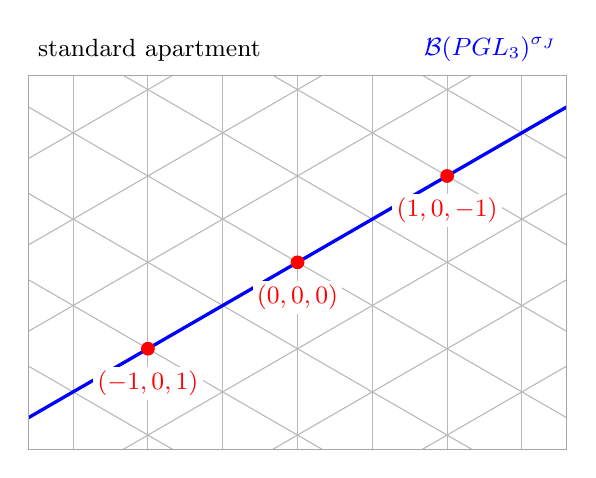
\begin{tikzpicture}[scale=0.95,>=Latex]
  \begin{scope}
    \clip (-3.6,-2.5) rectangle (3.6,2.5);
    \foreach \x in {-4,-3,-2,-1,0,1,2,3,4} {
      \draw[gray!55] (\x,-3) -- (\x,3);
    }
    \foreach \k in {-9,-8,-7,-6,-5,-4,-3,-2,-1,0,1,2,3,4,5,6,7,8,9} {
      \draw[gray!55] (-4,{-4*0.57735+1.1547*\k}) -- (4,{4*0.57735+1.1547*\k});
      \draw[gray!55] (-4,{4*0.57735+1.1547*\k}) -- (4,{-4*0.57735+1.1547*\k});
    }
    \draw[very thick,blue] (-4,-2.3094) -- (4,2.3094);
  \end{scope}
  \draw[gray!70] (-3.6,-2.5) rectangle (3.6,2.5);
  \foreach \x/\y in {-2/-1.1547,0/0,2/1.1547} {
    \filldraw[red] (\x,\y) circle (2.4pt);
  }
  \node[red,font=\small,fill=white,inner sep=1.5pt] at (-2,-1.62) {$(-1,0,1)$};
  \node[red,font=\small,fill=white,inner sep=1.5pt] at (0,-0.47) {$(0,0,0)$};
  \node[red,font=\small,fill=white,inner sep=1.5pt] at (2,0.69) {$(1,0,-1)$};
  \node[blue,font=\small,anchor=south east] at (3.6,2.55) {$\mathcal B(PGL_3)^{\sigma_J}$};
  \node[font=\small,anchor=south west] at (-3.6,2.55) {standard apartment};
\end{tikzpicture}
\caption{The orthogonal duality $\sigma_J$ folds the standard apartment of $PGL_3$ onto a fixed line. In the normalization of Proposition~\ref{prop:new-fold}, the fixed vertices are represented by $(m,0,-m)$.\label{fig:new-folded-apartment}}
\end{figure}

\subsection{The Prasad--Yu theorem and its precise scope}
Let $\Theta$ be a finite group of $F$-automorphisms of a connected
reductive $F$-group $\mathbf H$, and let
$\mathbf H_\Theta=(\mathbf H^\Theta)^\circ$ be the connected fixed
subgroup. The theorem of Prasad and Yu \cite[Theorem~1.9]{PY02}
identifies the Bruhat--Tits building of $\mathbf H_\Theta$ with the
$\Theta$-fixed point set in the building of $\mathbf H$, with the
appropriate geometric realization, provided $|\Theta|$ is prime to
the residue characteristic and the standard Bruhat--Tits hypotheses
hold. We use the theorem here only for split reductive groups over
nonarchimedean local fields. The theorem identifies \emph{geometric
points}; it does not assert a bijection between vertices in the two
original, unsubdivided simplicial structures.

\begin{proposition}[The untwisted orthogonal fixed building; cited]
\label{prop:new-PY}
Let $F$ have residue characteristic different from $2$. Let
$J=\left(\begin{smallmatrix}0&0&1\\0&-1&0\\1&0&0\end{smallmatrix}\right)$,
and let $\sigma_J(g)=J\,{}^tg^{-1}J$ on the split group
$\mathbf H=PGL_3$. The connected fixed group
$\mathbf H_{\sigma_J}$ is the split adjoint orthogonal group
$SO(J)\simeq PGL_2$ over $F$. There is a canonical identification,
compatible with the group action, of geometric buildings
\[
 \mathcal B\bigl(SO(J),F\bigr)
 \simeq \mathcal B\bigl(PGL_3,F\bigr)^{\sigma_J}.
\]
The right-hand side is one-dimensional and is a tree with its
inherited metric, possibly with a different simplicial subdivision.
\end{proposition}
\begin{proof}
The equation $\sigma_J(g)=g$ is the projective orthogonal-similitude
condition $g^tJg=\lambda J$. Its connected adjoint quotient is the
orthogonal group of the split, three-dimensional quadratic space.
The form is split because $e_1$ and $e_3$ span a hyperbolic plane.
The exceptional rank-one isomorphism identifies this connected group
with $PGL_2$. Since $\sigma_J$ has order two and the residue
characteristic is odd, the stated identification is exactly the
special case of \cite[Theorem~1.9]{PY02}. The building of split
$PGL_2$ is a tree.
\end{proof}

\begin{remark}
For residue characteristic $2$, the order of the involution is not
prime to the residue characteristic. We make no assertion using
\cite{PY02} in that case. Even for odd residue characteristic,
$\mathcal B(PGL_3)^{\sigma_J}$ is not the same object as
$\operatorname{Fix}(g\sigma_J)$ for general $g\in PGL_3(F)$.
The latter set can be empty, finite, or contain a different fixed
subcomplex. The historical counting arguments concern precisely the
latter sets.
\end{remark}

\subsection{The subcomplex $\mathcal Z$ is not the orthogonal tree}
The historical construction uses a decomposition
$V=V_A\oplus W_A$, with $\dim V_A=1$ and $\dim W_A=2$.
The corresponding Levi subgroup is the image of
$GL(V_A)\times GL(W_A)$ in $PGL(V)$. Its enlarged building is modeled
by a tree times a real line. The embedded subcomplex $\mathcal Z$
of Section~\ref{sec:4} inherits this two-dimensional structure.

\begin{proposition}[A dimension and invariance distinction]
\label{prop:new-Z}
Under a fixed decomposition $F^3=F e_0\oplus F^2$, the family of
lattices
\[
 \pi^n\mathcal O_Fe_0\oplus\Lambda,
 \qquad n\in\mathbb Z,\quad
 [\Lambda]\in\mathcal B(PGL_2,F)^{(0)},
\]
together with the connecting simplices, is a simplicial realization
of the standard Levi subbuilding (up to its usual subdivision). Its
geometric realization has dimension two. Consequently it cannot be
identified as a whole with the one-dimensional fixed-point building
in Proposition~\ref{prop:new-PY}. The separate condition that a
particular $A\tau$ preserves $\mathcal Z$ must be checked from $A$.
\end{proposition}
\begin{proof}
The building of $GL_2$ before quotienting by its split center
has a rank-one tree coordinate and a real determinant-valuation
coordinate. The single additional $GL_1$ factor contributes a second
central coordinate. Passing to the quotient by common scalar
homotheties removes one central coordinate, leaving the tree and one
real coordinate. The displayed lattices form a discrete lattice in
that product, and the incidence relations provide its simplicial
subdivision. An isomorphism with the fixed-point building in
Proposition~\ref{prop:new-PY} would preserve dimension, which is
impossible. No general involution invariance of $\mathcal Z$
follows from its construction.
\end{proof}

\begin{example}[A useful geometric diagram]
At a vertex $[\Lambda]$ of the $PGL_2$ tree, the points
$[\pi^n\mathcal O_Fe_0\oplus\Lambda]$ form a discrete vertical
line. Two adjacent tree vertices give two such lines, joined by the
triangulated strip in Figure~\ref{fig:4.6}. This explains why the
characteristic-leaf construction can start with an edge of a tree
and end with a two-dimensional triangle in $\mathcal Z$.
\end{example}

\subsection{Other involutions and their actual fixed sets}
A normalized twisted matrix action on lattice classes is
$T_A[L]=[A L^\vee]$. For a symmetric $A$ one has
$T_A^2[L]=[AA^{-t}L]=[L]$. It is therefore an involution on
$\mathcal B(PGL_3)$. It need not equal $\sigma_J$.

\begin{proposition}[A diagonal midpoint obstruction; direct proof]
\label{prop:new-diagonal}
Let $A=\operatorname{diag}(\pi^{d_1},\pi^{d_2},\pi^{d_3})$
with $d_i\in\mathbb Z$. On the standard apartment the fixed locus of
$T_A$ is the single geometric point represented by
$\tfrac12(d_1,d_2,d_3)$.
This point is an apartment vertex if and only if
$d_1\equiv d_2\equiv d_3\pmod 2$.
If the congruence fails, there is no fixed vertex \emph{in that
apartment}, even though the geometric action has a fixed point.
\end{proposition}
\begin{proof}
On apartment coordinates $T_A$ is the affine reflection
$\boldsymbol x\mapsto\boldsymbol d-\boldsymbol x$.
The fixed-point equation modulo the scalar line says
$2\boldsymbol x=\boldsymbol d+c(1,1,1)$ for some real $c$.
Modulo the scalar line this determines one point
$\boldsymbol d/2$. It is represented by an integer triple exactly
when all differences $(d_i-d_j)/2$ are integers. This is equivalent
to the stated parity congruence.
\end{proof}

\begin{example}[A fixed edge midpoint over $\mathbb Q_3$]
For $A=\operatorname{diag}(3,1,1)$ the point
$(\frac12,0,0)$ lies halfway along the edge from
$(0,0,0)$ to $(1,0,0)$ in the standard apartment. The involution
interchanges those endpoints and fixes no apartment vertex. It is
not legitimate to replace a midpoint fixed point by an ambient fixed
vertex without subdividing the edge. This is a local model for the
parity distinction in characteristic bases.
\end{example}

\subsection{Block representatives and their fixed vertices in $\mathcal Z$}
\label{sec:new-Zfix}

The representatives used in the running example have the block form
\eqref{eqn:4.11}. For such representatives the fixed vertices that lie
in $\mathcal Z$ can be found exactly, from the tree alone. The
statement is elementary; it does not describe the fixed vertices
outside $\mathcal Z$, which are the characteristic leaves.

\begin{proposition}[Fixed vertices in $\mathcal Z$; direct proof]
\label{prop:new-Zfix}
Let $w=\smat{0}{1}{-1}{0}$, let $B\in GL_2(F)$, and put $C=-Bw$ and
$A_a=\operatorname{diag}(a,C)$ for $a\in F^\times$, acting on
$V=Fe_0\oplus F^2$.
\begin{itemize}
\item[(a)] $C\,{}^tC^{-1}=-B^2/\det B$, and for every lattice
$\Lambda=M\mathcal O_F^2$ in $F^2$ and every $n\in\mathbb Z$,
\[
 A_a\bigl(\pi^n\mathcal O_Fe_0\oplus\Lambda\bigr)^\vee
 =a\pi^{-n}\mathcal O_Fe_0\oplus(\det M)^{-1}B\Lambda .
\]
\item[(b)] The class $[\pi^n\mathcal O_Fe_0\oplus\Lambda]$ is fixed by
$T_{A_a}$ if and only if $B\Lambda=\pi^s\Lambda$ for some
$s\in\mathbb Z$ and
\[
 2n=v_F(a)-s+v_F(\det M).
\]
In that case $v_F(\det B)=2s$.
\item[(c)] If $v_F(\det B)$ is odd, $T_{A_a}$ has no fixed vertex in
$\mathcal Z$. If $v_F(\det B)=2s$, then
$[\pi^n\mathcal O_Fe_0\oplus\Lambda]\mapsto[\Lambda]$ is a bijection
from $\operatorname{Fix}(T_{A_a})\cap\mathcal Z$ onto the set of
vertices $x$ of the tree with
\[
 Bx=x\qquad\text{and}\qquad t_2(x)\equiv v_F(a)+s\pmod 2 .
\]
In particular
$|\operatorname{Fix}(T_{A_1})\cap\mathcal Z|
+|\operatorname{Fix}(T_{A_\pi})\cap\mathcal Z|
=|\operatorname{Fix}(B)|$.
\item[(d)] If $e\in GL_2(F)$ commutes with $B$ and
$y=\operatorname{diag}(1,e)$, then
$yA_a\,{}^ty=\det(e)\,A_{a/\det e}$. Hence $A_a$ and $A_{a/\det e}$
are normalized representatives of $\sigma$-conjugate elements of
$PGL_3(F)$. When $F[B]=E$ is a quadratic field, this applies to every
$a/N_{E/F}(e)$ with $e\in E^\times$.
\end{itemize}
\end{proposition}
\begin{proof}
For $X\in GL_2(F)$ one has ${}^tX^{-1}=(\det X)^{-1}wXw^{-1}$.
(a) Since $\det C=\det B$ and $w^2=-1$,
\[
 C\,{}^tC^{-1}=(\det B)^{-1}(Bw)\,w\,(Bw)\,w^{-1}
 =(\det B)^{-1}B\,w^2\,B=-B^2/\det B .
\]
The dual of a direct sum of lattices in orthogonal summands is the
direct sum of the duals. The dual of $\pi^n\mathcal O_Fe_0$ is
$\pi^{-n}\mathcal O_Fe_0$, and
$\Lambda^\vee={}^tM^{-1}\mathcal O_F^2
=(\det M)^{-1}wMw^{-1}\mathcal O_F^2=(\det M)^{-1}w\Lambda$.
Then $C\Lambda^\vee=-(\det M)^{-1}Bw^2\Lambda=(\det M)^{-1}B\Lambda$.

(b) By (a), the class is fixed exactly when there is an integer $r$
with $a\pi^{-n}\mathcal O_F=\pi^{r+n}\mathcal O_F$ and
$(\det M)^{-1}B\Lambda=\pi^r\Lambda$. The second condition says
$B\Lambda=\pi^s\Lambda$ with $s=r+v_F(\det M)$, and the first says
$v_F(a)-n=r+n$. Taking determinants in $B\Lambda=\pi^s\Lambda$ gives
$v_F(\det B)=2s$.

(c) The first assertion follows from (b). Assume $v_F(\det B)=2s$. A
vertex $x=[\Lambda]$ of the tree is fixed by $B$ exactly when
$B\Lambda=\pi^s\Lambda$. By (b), for a given representative $\Lambda$
there is an $n$ making $[\pi^n\mathcal O_Fe_0\oplus\Lambda]$ a fixed
vertex exactly when $v_F(a)-s+v_F(\det M)$ is even, and $n$ is then
unique. Replacing $\Lambda$ by $\pi\Lambda$ replaces $v_F(\det M)$ by
$v_F(\det M)+2$ and $n$ by $n+1$, which gives the same vertex of
$\mathcal Z$. So the map is well defined and bijective onto the
vertices with $t_2(x)\equiv v_F(a)+s$. The two parities are realized
by $a=1$ and $a=\pi$.

(d) Since $w\,{}^te\,w^{-1}=\det(e)\,e^{-1}$ and $e$ commutes with
$B$,
\[
 e\,C\,{}^te=-eBw\,{}^te=-\det(e)\,eBe^{-1}w=\det(e)\,C .
\]
So $yA_a\,{}^ty=\operatorname{diag}(a,\det(e)C)=\det(e)A_{a/\det e}$.
If $g=[A J]$ and $x\in PGL_3(F)$, then $x^{-1}g\sigma_J(x)$ has
normalized representative $x^{-1}A\,{}^tx^{-1}$; take $x=y^{-1}$.
For $e\in E^\times=F[B]^\times$ the determinant is $N_{E/F}(e)$.
\end{proof}

\begin{runex}[The fixed vertices in $\mathcal Z$ for the specimens]
\label{run:Zfix}
In all four specimens $\det B$ is a unit ($2$, $1$, $10$, $-2$), so
$s=0$, and Proposition~\ref{prop:new-Zfix}(c) says: $T_{A_a}$ has one
fixed vertex in $\mathcal Z$ over each vertex $x$ of the tree with
$Bx=x$ and $t_2(x)\equiv v_3(a)$.
\begin{itemize}
\item Specimens I and II: $B$ is $\smat{1}{-1}{1}{1}$ or
$\smat{0}{-1}{1}{0}$ modulo $3$, with irreducible characteristic
polynomial, so $B$ fixes only $[\Lambda_0]$, of type $0$. Hence
$\operatorname{Fix}(T_{A_1})\cap\mathcal Z=\{[L_0]\}$ and
$\operatorname{Fix}(T_{A_3})\cap\mathcal Z=\emptyset$.
\item Specimen III: $B\equiv1$ modulo $3$ fixes $[\Lambda_0]$ and its
four neighbors, and no other vertex. The center has type $0$ and the
neighbors type $1$. Hence $T_{A_1}$ fixes $[L_0]$ only, and $T_{A_3}$
fixes the four vertices $[3\mathbb Z_3e_0\oplus\Lambda]$ with
$n=(1-0+1)/2=1$.
\item Specimen IV: $B\equiv\smat{1}{0}{1}{1}$ modulo $3$ fixes
$[\Lambda_0]$ and $p'=[3\mathbb Z_3e_1+\mathbb Z_3e_2]$, the two ends
of one edge. Hence $T_{A_a}$ fixes $[L_0]$ when $v_3(a)$ is even and
$[3\mathbb Z_3e_0\oplus(3\mathbb Z_3e_1+\mathbb Z_3e_2)]$ when
$v_3(a)$ is odd.
\end{itemize}
By part (d), $A_1$ and $A_6$ are $\sigma$-conjugate over
$\mathbb Q_3$ in specimen~IV, since $6=N_{E/F}(3+\sqrt3)$; this is
consistent with the counts, and it shows that the two vertices above
are exchanged by a twisted conjugation. In none of the specimens does
$\sigma_J$ itself play a role: the fixed sets are those of the
twisted elements $T_{A_a}$, and they are finite, whereas
$\mathcal B(PGL_3)^{\sigma_J}$ is a tree.
\end{runex}

\begin{draftremark}[Scope of the fixed-point comparison]
The preceding propositions do not establish an identification
between $\operatorname{Fix}(A\tau)$ and the fixed vertices of the
norm element $h\in H_1(F)$ or $h'\in H_2(F)$. That correspondence
requires the characteristic-base, characteristic-leaf, and
stabilizer arguments in Lemmas~\ref{lemma:4.9}, \ref{lemma:4.13},
\ref{lemma:4.16}, and \ref{lemma:4.18}. Those are separate
verification obligations.
\end{draftremark}

\section{Vertex types, tree parity, and quadratic characters}
\label{sec:new-types}

The type map on a $PGL_3$ building is a very cheap invariant: it
remembers only the determinant valuation modulo three. Yet it gives a
necessary condition for a twisted fixed vertex, without any use of
the complicated characteristic-leaf classification. The analogous
modulo-two invariant on the $PGL_2$ tree explains fixed edge
midpoints and the appearance of ramified parity corrections; see Figure~\ref{fig:new-tree-parity}.

\begin{figure}[htbp]
\centering
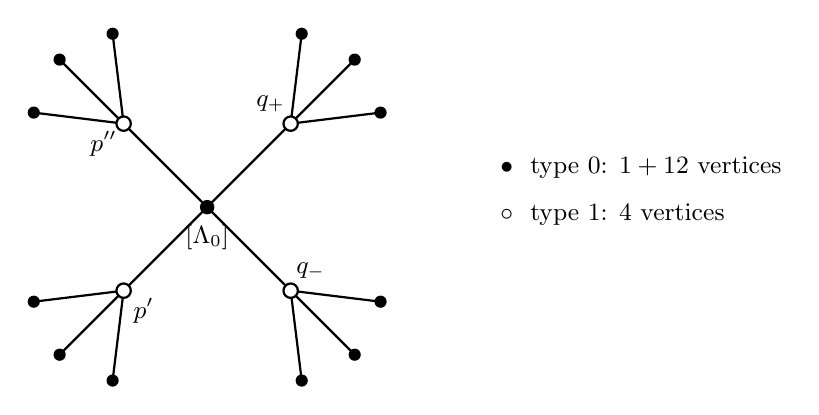
\begin{tikzpicture}[scale=1.0,>=Latex]
  \coordinate (O) at (0,0);
  \foreach \a/\lab in {45/{$q_+$},135/{$p''$},225/{$p'$},315/{$q_-$}} {
    \path (O) ++(\a:1.5) coordinate (N\a);
    \draw[thick] (O) -- (N\a);
    \foreach \b in {-38,0,38} {
      \path (N\a) ++(\a+\b:1.15) coordinate (M\a\b);
      \draw[thick] (N\a) -- (M\a\b);
      \fill (M\a\b) circle (2.2pt);
    }
    \filldraw[fill=white,thick] (N\a) circle (2.6pt);
    \node[font=\small] at ($(N\a)+(\a+90:0.36)$) {\lab};
  }
  \fill (O) circle (2.6pt);
  \node[font=\small,below=3pt] at (O) {$[\Lambda_0]$};
  \node[font=\small,align=left,anchor=west] at (3.6,0.5) {$\bullet$\ \ type $0$: $1+12$ vertices};
  \node[font=\small,align=left,anchor=west] at (3.6,-0.1) {$\circ$\ \ type $1$: $4$ vertices};
\end{tikzpicture}
\caption{The ball of radius $2$ about $[\Lambda_0]$ in the tree of
$PGL_2(\mathbb Q_3)$, with vertices marked by type. Adjacent vertices
have different types, so a transformation that exchanges the types
fixes no vertex. In the running example the two types of a fixed ball
correspond to the two rational twisted classes: $1$ and $4$ vertices
for radius $1$, and $13$ and $4$ for radius $2$.\label{fig:new-tree-parity}}
\end{figure}

\subsection{The type congruence}
For a rank-$n$ lattice $L=M\mathcal O_F^n$, set
\begin{equation}\label{eq:new-type}
 t_n([L])=v_F(\det M)\pmod n\ \in\mathbb Z/n\mathbb Z.
\end{equation}
A different basis of $L$ changes $\det M$ by a unit. Multiplication
of $L$ by $\pi^r$ changes the determinant valuation by $nr$, so the
class is well-defined.

\begin{proposition}[Twisted type obstruction; direct proof]
\label{prop:new-type}
For any $A\in GL_n(F)$ and any vertex $[L]$ of the
$PGL_n(F)$ building,
\begin{equation}\label{eq:new-type-transform}
 t_n([A L^\vee])\equiv v_F(\det A)-t_n([L])\pmod n.
\end{equation}
In particular, a fixed vertex of $T_A:[L]\mapsto[A L^\vee]$
necessarily satisfies
\begin{equation}\label{eq:new-type-obstruction}
 2t_n([L])\equiv v_F(\det A)\pmod n.
\end{equation}
For $n=3$ the possible type is uniquely prescribed. For $n=2$
the condition requires $v_F(\det A)$ even.
\end{proposition}
\begin{proof}
Write $L=M\mathcal O_F^n$. Then
$L^\vee=M^{-t}\mathcal O_F^n$, so
$v_F(\det(AM^{-t}))=v_F(\det A)-v_F(\det M)$.
Reducing modulo $n$ proves \eqref{eq:new-type-transform}. If the
vertices are equal, their types agree, giving
\eqref{eq:new-type-obstruction}. As $2$ is invertible modulo $3$,
there is one solution in $\mathbb Z/3\mathbb Z$.
For $n=2$ the left side vanishes modulo two.
\end{proof}

\begin{example}[Three types over $\mathbb Q_3$]
With $L_0=\mathbb Z_3^3$, the three vertices
\[
 [L_0],\quad
 [3\mathbb Z_3e_1+\mathbb Z_3e_2+\mathbb Z_3e_3],\quad
 [3\mathbb Z_3e_1+3\mathbb Z_3e_2+\mathbb Z_3e_3]
\]
have types $0,1,2$ respectively. With $A=I$, duality can fix only
type $0$ vertices. With $A=\operatorname{diag}(3,1,1)$, the only
possible fixed type is $2$, because $2\cdot2\equiv1\pmod3$.
These are necessary, not sufficient, conditions.
\end{example}

\subsection{Bipartition of the tree and edge inversions}
On the $PGL_2$ tree, vertices are colored by
$t_2([L])\in\mathbb Z/2\mathbb Z$. Every edge joins opposite colors.
An element of $PGL_2(F)$ represented by $B$ shifts both colors by
$v_F(\det B)\bmod2$.

\begin{proposition}[Odd determinant and fixed vertices; direct proof]
\label{prop:new-tree-parity}
Let $B\in GL_2(F)$. If $v_F(\det B)$ is odd, the induced
action on the $PGL_2$ tree fixes no vertex. It may fix the
midpoint of an edge, but need not fix any geometric point. If it
fixes a geometric point, then it fixes the midpoint of an edge
setwise inverted by the action.
\end{proposition}
\begin{proof}
For any lattice $L$, $t_2([BL])=t_2([L])+v_F(\det B)$
modulo two. Odd valuation exchanges the two colors and prevents a
fixed vertex. A tree is a union of closed edges. If an isometry
fixes a point in the interior of an edge, it preserves that edge
setwise. Since it exchanges the endpoint colors, it must swap the
endpoints and fix their midpoint. There can also be actions with
no fixed point, such as an odd-length translation along an apartment.
\end{proof}

\begin{example}[Actual edge inversion over $\mathbb Q_3$]
\label{ex:new-edge}
Set $B=\left(\begin{smallmatrix}0&1\\3&0\end{smallmatrix}\right)$.
Then $B^2=3I$ and $v_3(\det B)=1$.
It exchanges $[\mathbb Z_3^2]$ and
$[\mathbb Z_3 e_1+3\mathbb Z_3 e_2]$, an adjacent pair.
It fixes their midpoint but not either endpoint. In contrast,
$\operatorname{diag}(3,1)$ has odd determinant valuation but
translates along an apartment, so it has no fixed geometric point.
\end{example}

\begin{runex}[Types of the fixed vertices]
\label{run:types}
Proposition~\ref{prop:new-type} can be tested on every fixed vertex
found so far. For $A_1$ in specimens I, II, III and IV,
$v_3(\det A_1)=0$, so a fixed vertex must have type $0$. Indeed
$[L_0]$ has type $0$, and the leaves $L_\pm$, $L'_\pm$ of
Running example~\ref{run:leaves} have determinant valuation
$0+1+2=3\equiv0$. For $A_3$, $v_3(\det A_3)=1$ and the type must be
$2$, because $2\cdot2\equiv1\pmod3$. The four fixed vertices
$[3\mathbb Z_3e_0\oplus\Lambda]$ of specimen~III have determinant
valuation $1+1=2$, and so does the fixed vertex of $T_{A_3}$ in
specimen~IV. The congruence does not see the difference between
specimens I and III for $a=3$: type $2$ is allowed in both, but
$T_{A_3}$ has no fixed vertex in specimen~I and four in specimen~III.

For the tree, Proposition~\ref{prop:new-tree-parity} applies to
specimen~IV: $\det h'=6$ has odd valuation, so $h'$ exchanges the two
types and fixes no vertex. It does fix the midpoint of the edge
joining $[\Lambda_0]$ and $p'$, the edge fixed pointwise by $h$.
\end{runex}

\subsection{Norm characters and explicit residue-field tests}
For a quadratic extension $E=F(\sqrt\epsilon)$, local class field
theory or the Hilbert norm theorem identifies the quadratic character
of $F^\times/N_{E/F}(E^\times)$ with
$\chi_E(a)=(a,\epsilon)_2$. This is the sign character that
occurs in the historical parametrization \eqref{eqn:3.18} up to the
global choice of transfer-factor sign.

\begin{proposition}[The unramified parity character; standard fact]
\label{prop:new-unram-char}
If $E/F$ is the unramified quadratic extension, then
\[
 N_{E/F}(E^\times)=\pi^{2\mathbb Z}\mathcal O_F^\times,
 \qquad \chi_E(a)=(-1)^{v_F(a)}.
\]
Thus the signed summation over norm classes amounts to subtracting
the odd-valuation contribution from the even-valuation contribution.
\end{proposition}
\begin{proof}
The extension of residue fields has norm map
$\mathbb F_{q^2}^\times\to\mathbb F_q^\times$ given by
$x\mapsto x^{q+1}$, which is surjective. Successive approximation
on principal units shows every unit of $F$ is a norm in an
unramified extension. A uniformizer of $F$ remains a uniformizer of
$E$, and its norm has valuation two. Therefore the valuations of
norms are exactly the even integers, proving the formula.
\end{proof}

\begin{example}[Ramified square classes over $\mathbb Q_3$ and
$\mathbb Q_5$]
For $E=\mathbb Q_3(\sqrt3)$ and $a=3^r u$ with
$u\in\mathbb Z_3^\times$, the odd-prime Hilbert-symbol formula gives
\[
 \chi_E(a)=(a,3)_3=(-1)^r\left(\frac{\bar u}{3}\right).
\]
Thus $\chi_E(2)=-1$, $\chi_E(3)=-1$, and
$\chi_E(6)=+1$. For $E=\mathbb Q_5(\sqrt5)$,
\[
 \chi_E(5^r u)=(5^r u,5)_5=\left(\frac{\bar u}{5}\right),
\]
so $\chi_E(2)=-1$ but $\chi_E(5)=+1$.
Here the parenthesized expressions are Legendre symbols.
Ramification therefore changes the valuation-parity rule: a unit
square class also matters. These computations describe the norm
character; they do not settle the external sign in the definition
of $S(0)$.
\end{example}

\begin{draftremark}[The remaining sign]
Formula~\eqref{eqn:3.18} involves an initial $\pm$ that is not
fixed by the character $\chi_E$. The identification of
$\chi_E$ with a signed difference of norm classes is exact, but
it proves neither the absolute normalization of the orbital
integrals nor the choice of the initial $\pm$. In particular,
Proposition~\ref{prop:5.6} cannot be promoted from
$|S(0)|=s(0)$ to $S(0)=s(0)$ on the basis of parity alone.
\end{draftremark}

\section{Finite projective geometry and the factor $Q$}
\label{sec:new-flags}

The constant
$Q=(1+q^{-1})(1+q^{-1}+q^{-2})$
first enters the historical reduction through the spherical
normalization. The finite incidence geometry of the link of a
hyperspecial vertex explains the numerical factor exactly and
also explains why it is a natural factor in Iwahori averaging.
We distinguish that theorem from the additional measure comparisons
needed for orbital-integral transfer.

\subsection{Flags and chambers in a vertex link}
Fix $x=[L]$ with $L=\mathcal O_F^3$. Vertices adjacent to $x$
correspond to proper nonzero subspaces of
$\bar L=L/\pi L\simeq\mathbb F_q^3$:
lines and planes. Two such neighbors are joined by a chamber
with $x$ precisely when the corresponding line is contained in
the corresponding plane. This is the incidence graph of
$PG(2,q)$, the spherical building of $PGL_3(\mathbb F_q)$.
Figure~\ref{fig:new-flag-chamber} shows schematically how a complete flag in the link corresponds to a chamber of the affine building.


\begin{figure}[htbp]
\centering
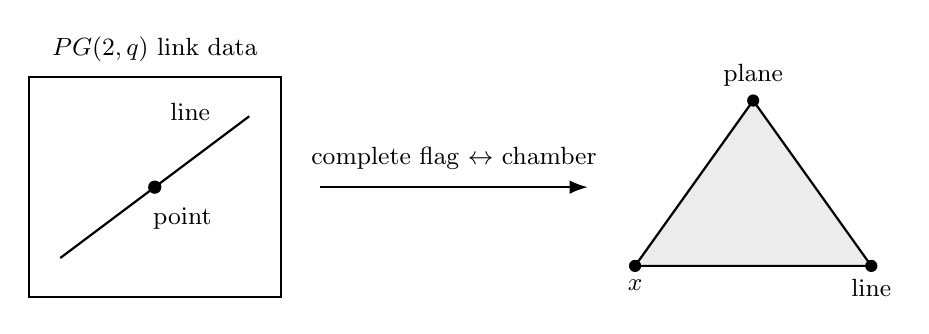
\begin{tikzpicture}[scale=1.0,>=Latex]
  \draw[thick] (-5.4,-1.4) rectangle (-2.2,1.4);
  \node[font=\small] at (-3.8,1.75) {$PG(2,q)$ link data};
  \draw[thick] (-5.0,-0.9) -- (-2.6,0.9);
  \fill (-3.8,0) circle (2.4pt);
  \node[font=\small] at (-3.45,-0.4) {point};
  \node[font=\small] at (-3.35,0.95) {line};
  \draw[->,thick] (-1.7,0) -- (1.7,0);
  \node[font=\small,above] at (0,0.1) {complete flag $\leftrightarrow$ chamber};
  \draw[thick,fill=gray!15] (2.3,-1.0) -- (3.8,1.1) -- (5.3,-1.0) -- cycle;
  \fill (2.3,-1.0) circle (2.2pt);
  \fill (3.8,1.1) circle (2.2pt);
  \fill (5.3,-1.0) circle (2.2pt);
  \node[font=\small,below] at (2.3,-1.05) {$x$};
  \node[font=\small,above] at (3.8,1.15) {plane};
  \node[font=\small,below] at (5.3,-1.05) {line};
\end{tikzpicture}
\caption{The factor $[K:I]$ counts complete flags in the link of a hyperspecial vertex. On the left is schematic finite-projective incidence data; on the right the corresponding chamber through the affine vertex $x$.\label{fig:new-flag-chamber}}
\end{figure}


\begin{proposition}[Flags, chambers, and Iwahori index; direct proof]
\label{prop:new-Q}
Let $K=PGL_3(\mathcal O_F)$ and let $I$ be the preimage of a
Borel subgroup $B(\mathbb F_q)$ under reduction
$K\to PGL_3(\mathbb F_q)$. Then
\begin{align}
 [K:I]&=(q^2+q+1)(q+1),\label{eq:new-index}\\
 q^{-3}[K:I]
 &=1+2q^{-1}+2q^{-2}+q^{-3}
 =Q.\label{eq:new-Q}
\end{align}
The first number is the number of complete flags (and hence of
chambers) in the spherical link of a vertex of the affine building.
\end{proposition}
\begin{proof}
There are $(q^3-1)/(q-1)=q^2+q+1$ lines in
$\mathbb F_q^3$. A plane containing a given line corresponds to a
line in the two-dimensional quotient; there are $q+1$ such planes.
Hence the number of incident line-plane pairs is
$(q^2+q+1)(q+1)$.
Reduction modulo $\pi$ identifies $K/I$ with
$PGL_3(\mathbb F_q)/B(\mathbb F_q)$; the latter homogeneous space
parametrizes complete flags. The index follows. Expanding and
dividing by $q^3$ gives \eqref{eq:new-Q}.
\end{proof}

\begin{proposition}[Weyl-length explanation; direct proof]
\label{prop:new-Weyl}
For the Weyl group $W=S_3$ with Coxeter length $\ell$,
\begin{equation}\label{eq:new-poincare}
 Q=\sum_{w\in W}q^{-\ell(w)}.
\end{equation}
Consequently $Q$ is the Poincar\'e polynomial of the finite
Weyl group evaluated at $q^{-1}$.
\end{proposition}
\begin{proof}
The six permutations in $S_3$ have lengths
$0,1,1,2,2,3$. Their generating polynomial is
$1+2t+2t^2+t^3=(1+t)(1+t+t^2)$.
Substitute $t=q^{-1}$ and use \eqref{eq:new-Q}.
\end{proof}

\begin{example}[The link for $\mathbb Q_3$ and $\mathbb Q_5$]
Over $\mathbb Q_3$ the plane $PG(2,3)$ has $13$ points and
$13$ lines, with four lines through each point. Thus
$[K:I]=52$ and $Q=52/27$.
Over $\mathbb Q_5$ there are $31$ points, six lines through each,
$[K:I]=186$, and $Q=186/125$.
These are rational normalization factors, not integer counts of
fixed vertices.
\end{example}

\begin{runex}[The factor $Q$ in the specimens]
\label{run:flags}
Every unit-element quantity of the running example is a vertex count
times $Q=52/27=3^{-3}\cdot52$. For specimen~III,
$r(0)=R(0)=5\cdot52/27=260/27$ and $s(0)=52/27$. The twisted
transformations act on the link of a fixed vertex by a correlation:
by \eqref{eq:run-Zaction}, $T_{A_1}$ sends the neighbor
$[\mathbb Z_3e_0\oplus3\Lambda_0]$ of $[L_0]$, attached to the line
spanned by $e_0$, to the neighbor $[3\mathbb Z_3e_0\oplus\Lambda_0]$,
attached to the plane spanned by $e_1,e_2$. So the $13$ line-neighbors
and the $13$ plane-neighbors of $[L_0]$ are exchanged, and the factor
$Q$ comes from the normalization of the spherical function, not from
counting neighbors or chambers fixed by $T_{A_a}$.
\end{runex}

\subsection{What is, and is not, normalized by incidence}
Normalize Haar measure on $PGL_3(F)$ by
$\operatorname{vol}(K)=1$. Then
$\operatorname{vol}(I)=[K:I]^{-1}$.
For a compact open subgroup $J$, let $e_J=1_J/\operatorname{vol}(J)$.
Here $e_K=1_K$, while $e_I=[K:I]1_I$.

\begin{proposition}[Iwahori-to-spherical averaging; direct proof]
\label{prop:new-averaging}
With the preceding Haar convention,
\begin{equation}\label{eq:new-averaging}
 e_K=\frac1{[K:I]}\sum_{kI\in K/I}{}^k e_I,
 \qquad ({}^k e_I)(g)=e_I(k^{-1}g).
\end{equation}
This is an exact identity of locally constant compactly supported
functions, not merely an equality of their integrals.
\end{proposition}
\begin{proof}
The cosets $kI$ partition $K$. Since
${}^k e_I=[K:I]1_{kI}$, the right-hand side is
$\sum_{kI}1_{kI}=1_K=e_K$.
\end{proof}

\begin{remark}
The identity \eqref{eq:new-averaging} gives a concrete geometric
reason that the same finite flag count appears when an Iwahori
computation is averaged to a spherical one. It does \emph{not}
show by itself that the old formula \eqref{eqn:3.17} contains
precisely the factor $Q$ in every nonunit double coset. Establishing
that requires the Macdonald spherical transform \cite{Ma71}, the
Jacobian, and the quotient Haar measures in Sections~\ref{sec:2}
and \ref{sec:3}. In particular the flag count cannot determine the
transfer-factor sign.
\end{remark}

\subsection{An incidence calculation for rank-two Hecke steps}
Define two operators on finitely supported functions on building
vertices. For $i=1,2$ put
\[
 (U_if)([L])=
 \sum_{\substack{\pi L\subsetneq M\subsetneq L\\
             \dim_{\mathbb F_q}(L/M)=i}}
 f([M]).
\]
Because the intermediate lattices have a unique normalized
representative between $\pi L$ and $L$, the sums are unambiguous.

\begin{proposition}[A two-step path identity; direct proof]
\label{prop:new-U1}
For a vertex $x=[L]$, the operator $U_1$ has exactly
$q^2+q+1$ outgoing neighbors, and so does $U_2$. Moreover,
\begin{equation}\label{eq:new-U1}
 U_1^2=(q+1)U_2+U_{(2,0,0)},
\end{equation}
where $U_{(2,0,0)}$ sums over lattice classes represented,
relative to $L$, by sublattices of elementary divisor type
$(2,0,0)$; the notation denotes the $PGL_3(F)$-equivariant
operator so defined.
\end{proposition}
\begin{proof}
Choosing $M$ with $[L:M]=q$ amounts to choosing a plane in
$L/\pi L$, of which there are $q^2+q+1$. Index-$q^2$
intermediate lattices correspond to lines in the same vector
space and are equally numerous.
For $U_1^2$ count chains
$L\supset M_1\supset M_2$ with both successive indices $q$.
By Smith normal form, the elementary divisors of $M_2$ in $L$
are either $(1,1,0)$ or $(2,0,0)$. In the first case
$L/M_2\simeq\mathbb F_q^2$, and the intermediate lattices
correspond to its $q+1$ one-dimensional subspaces.
In the second case $L/M_2\simeq\mathcal O_F/\pi^2$ and there
is exactly one index-$q$ intermediate submodule. Thus the
coefficient of each endpoint is $q+1$ or $1$, respectively,
which is precisely \eqref{eq:new-U1}.
\end{proof}

\begin{example}[An explicit two-step count for $q=3$]
Starting at $[\mathbb Z_3^3]$, there are $13$ first steps of
type $1$ and hence $13^2=169$ ordered two-step paths.
There are $13$ endpoints of type $(1,1,0)$, each reached by
$4$ paths. The remaining $117$ paths end at distinct
$(2,0,0)$ endpoints. Thus $169=13\cdot4+117$.
This is a directly checkable rank-two analogue of the tree's
adjacency recurrence, but unlike the tree it has two Cartan
orbits already at distance two.
\end{example}

\section{Tree adjacency, spherical Hecke operators, and the adjoint map}
\label{sec:new-hecke}

The rank-one building is not only a geometric counting space.
Its adjacency algebra is the spherical Hecke algebra of $PGL_2$.
This gives efficient recurrences for fixed-radius balls and
spectral interpretations of the split Satake restriction. The
rank-two calculation in Proposition~\ref{prop:new-U1} indicates
exactly why a single adjacency recurrence cannot replace all
of the original $PGL_3$ Satake coefficients.

\subsection{Distance operators on the regular tree}
Let $\mathcal T$ denote the $(q+1)$-regular tree of $PGL_2(F)$.
For a finitely supported function $f$ on vertices define
\[
 (D_nf)(x)=\sum_{d(x,y)=n}f(y),\qquad n\geq0,
 \qquad A_{\mathcal T}=D_1.
\]
The operator $A_{\mathcal T}$ is ordinary adjacency. Its powers
count walks, not necessarily nonbacktracking walks.

\begin{proposition}[Distance recurrence and generating series;
direct proof]\label{prop:new-D}
On any $(q+1)$-regular tree,
\begin{align}
 D_0&=1,\qquad D_1=A_{\mathcal T},\nonumber\\
 A_{\mathcal T}D_1&=D_2+(q+1)D_0,\label{eq:new-D1}\\
 A_{\mathcal T}D_n&=D_{n+1}+qD_{n-1}\quad(n\geq2).
 \label{eq:new-Dn}
\end{align}
In the ring of formal power series with operator coefficients,
\begin{equation}\label{eq:new-Dgen}
 \sum_{n\geq0}D_nu^n
 =\frac{1-u^2}{1-A_{\mathcal T}u+qu^2}.
\end{equation}
Here the quotient means multiplication by the formal inverse
of the denominator.
\end{proposition}
\begin{proof}
A walk of length two from $x$ to itself first chooses one of
$q+1$ neighbors and then returns, whereas a vertex at distance
two has a unique length-two geodesic. This proves
\eqref{eq:new-D1}. For $n\geq2$, fix $x,y$. If
d$(x,y)=n+1$, exactly one neighbor of $x$ lies at distance $n$
from $y$. If $d(x,y)=n-1$, exactly $q$ neighbors of $x$ lie at
distance $n$ from $y$. There are no other possibilities,
proving \eqref{eq:new-Dn}. Multiply $\sum D_nu^n$ by
$1-A_{\mathcal T}u+qu^2$. The constant coefficient is $1$,
the coefficient of $u$ vanishes, the coefficient of $u^2$
is $-1$ by \eqref{eq:new-D1}, and all higher coefficients
vanish by \eqref{eq:new-Dn}. This gives \eqref{eq:new-Dgen}.
\end{proof}

\begin{example}[The second sphere]
On the $4$-regular tree of $PGL_2(\mathbb Q_3)$,
$D_2=A_{\mathcal T}^2-4$. The sphere of radius two about
a vertex contains $4\cdot3=12$ vertices. Over $\mathbb Q_5$,
$D_2=A_{\mathcal T}^2-6$ and the sphere contains $30$
vertices. These equalities are valid before any spectral
decomposition or choice of Haar measure.
\end{example}

\begin{runex}[Spheres about $\lbrack\Lambda_0\rbrack$]
\label{run:hecke}
On the $4$-regular tree of $PGL_2(\mathbb Q_3)$ the spheres about
$[\Lambda_0]$ have $1,4,12,36,\dots$ vertices. The sphere of radius
$1$ is $\{p',p'',q_+,q_-\}$. In specimen~III the matrix $B$ fixes the
ball of radius $1$, and in the deeper specimen
$B=1+9\smat{0}{-1}{1}{0}$ it fixes the ball of radius $2$, with
$1+4+12=17$ vertices. Applied to the constant function, the operators
of Proposition~\ref{prop:new-D} give these numbers:
$D_0\mathbf 1=\mathbf 1$, $D_1\mathbf 1=4\cdot\mathbf 1$,
$D_2\mathbf 1=12\cdot\mathbf 1$. The alternating combination
$D_0-D_1+D_2$ gives $1-4+12=9=3^2$. This alternating sum, not the
plain sum, is what the two rational classes of the twisted side
compute (Proposition~\ref{prop:new-parity}).
\end{runex}

\subsection{The spherical Hecke algebra}
Let $K_2=PGL_2(\mathcal O_F)$ and normalize Haar measure by
$\operatorname{vol}(K_2)=1$. The characteristic function of
$K_2\operatorname{diag}(\pi,1)K_2$ acts on vertex functions
as $A_{\mathcal T}$. Its convolution powers therefore satisfy
\eqref{eq:new-D1}--\eqref{eq:new-Dn} after collecting the
relevant distance-double-coset terms. Under the normalized
Satake transform, its eigenvalue on an unramified principal series
with parameter $\operatorname{diag}(z,z^{-1})\in SL_2(\mathbb C)$
is $q^{1/2}(z+z^{-1})$; this eigenvalue convention corresponds to
the unnormalized adjacency operator on the tree.

\begin{proposition}[A Satake character identity; direct proof]
\label{prop:new-adjoint-satake}
Let $s=\operatorname{diag}(z,z^{-1})\in SL_2(\mathbb C)$.
The three-dimensional adjoint representation
$\operatorname{Sym}^2(\mathrm{Std})$ has character
\begin{equation}\label{eq:new-adjoint-char}
 \operatorname{tr}(\operatorname{Sym}^2(s))=z^2+1+z^{-2}.
\end{equation}
For its image in $SL_3(\mathbb C)$, both the defining and
its dual representation have the same character.
Consequently the two fundamental $SL_3$ characters pull back
to the same Laurent polynomial along the adjoint $L$-map.
\end{proposition}
\begin{proof}
The weights of $\operatorname{Sym}^2$ are the pairwise products
$z\cdot z$, $z\cdot z^{-1}$, and $z^{-1}\cdot z^{-1}$.
Thus the eigenvalues are $z^2,1,z^{-2}$, proving
\eqref{eq:new-adjoint-char}. Their product is one. The dual
eigenvalues are the inverses, which form the same multiset.
The two fundamental representations of $SL_3$ are its defining
representation and the dual of that representation. Their
restricted characters coincide.
\end{proof}

\begin{example}[A normalized versus unnormalized eigenvalue]
At $z=1$, the expression in \eqref{eq:new-adjoint-char} equals
$3$, while adjacency on the $q+1$-regular tree sends the constant
function to $(q+1)$ times that function. This is not a contradiction:
$z=1$ is a particular Satake parameter and is not the parameter
of the constant representation under the normalized convention.
Keeping the factor $q^{1/2}$ and the modular character explicit
prevents an accidental replacement of adjacency by a representation
character.
\end{example}

The identity \eqref{eq:new-adjoint-char} is a concrete
spectral formulation of the restriction of characters in
Section~\ref{sec:2}. It is not a proof of the twisted
fundamental lemma. That lemma compares orbital integrals, whereas
Satake pullback by itself compares spherical Hecke functions.
A full alternative proof in the split case would have to identify
the twisted orbital transform with the restricted spherical
transform, including the Jacobian in Section~\ref{sec:2}.

\section{Discrete ball counts and the nonsplit signed difference}
\label{sec:new-counts}

We now isolate a finite combinatorial identity that is visible inside
the historical nonsplit comparison. Unlike the endoscopic fixed-point
claims themselves, this identity has a short independent proof.
It explains the appearance of the power $q^m$ in the final
calculation and suggests a systematic generating-function approach.

\subsection{Two sorts of centers in a tree}
For $m\geq0$, let $B_v(m)$ denote the number of vertices in the
closed radius-$m$ ball about a vertex of the $(q+1)$-regular tree.
Let $B_e(m)$ denote the number of vertices at distance at most $m-\tfrac12$
from the midpoint of a chosen edge, with $B_e(0)=0$.
Equivalently, in each of the two half-trees obtained by removing
the interior of the edge, count vertices at distance at most
$m-1$ from that half-tree's endpoint. The two contributions
are disjoint. Figure~\ref{fig:new-tree-balls} illustrates the two kinds of centers whose ball counts are compared below.


\begin{figure}[htbp]
\centering
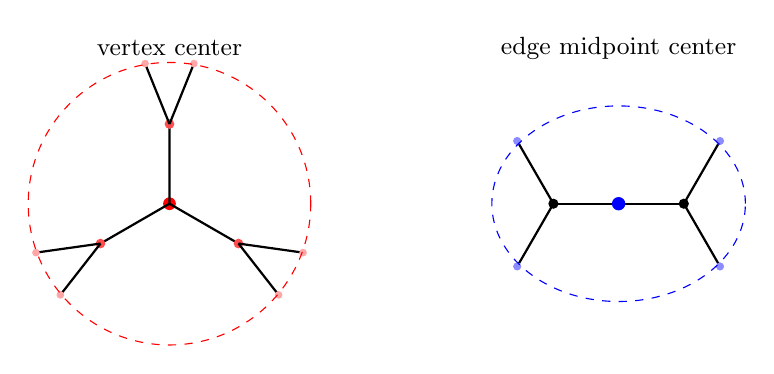
\begin{tikzpicture}[scale=0.92,>=Latex]
  \node[font=\small] at (-3.1,2.15) {vertex center};
  \fill[red] (-3.1,0) circle (2.5pt);
  \foreach \a in {90,210,330} {
    \path (-3.1,0) ++(\a:1.1) coordinate (A\a);
    \draw[thick] (-3.1,0) -- (A\a);
    \fill[red!70] (A\a) circle (1.9pt);
    \foreach \b in {-22,22} {
      \path (A\a) ++(\a+\b:0.9) coordinate (B\a\b);
      \draw[thick] (A\a) -- (B\a\b);
      \fill[red!35] (B\a\b) circle (1.5pt);
    }
  }
  \draw[red,dashed] (-3.1,0) circle (1.95);
  \node[font=\small] at (3.1,2.15) {edge midpoint center};
  \coordinate (L) at (2.2,0); \coordinate (R) at (4.0,0);
  \draw[thick] (L) -- (R);
  \fill (L) circle (2pt); \fill (R) circle (2pt);
  \filldraw[blue] ($(L)!0.5!(R)$) circle (2.4pt);
  \foreach \a in {120,240} {
    \path (L) ++(\a:1.0) coordinate (LL\a);
    \draw[thick] (L) -- (LL\a);
    \fill[blue!45] (LL\a) circle (1.6pt);
  }
  \foreach \a in {60,-60} {
    \path (R) ++(\a:1.0) coordinate (RR\a);
    \draw[thick] (R) -- (RR\a);
    \fill[blue!45] (RR\a) circle (1.6pt);
  }
  \draw[blue,dashed] (3.1,0) ellipse (1.75 and 1.35);
\end{tikzpicture}
\caption{The two counting centers used in Proposition~\ref{prop:new-ball}. A vertex-centered ball and an edge-midpoint-centered ball have different cardinalities, and their difference is exactly $q^m$.\label{fig:new-tree-balls}}
\end{figure}


\begin{proposition}[Vertex versus edge centers; direct proof]
\label{prop:new-ball}
For every integer $m\geq0$,
\begin{align}
 B_v(m)&=1+(q+1)\frac{q^m-1}{q-1}
       =\frac{q^{m+1}+q^m-2}{q-1},\label{eq:new-Bv}\\
 B_e(m)&=2\frac{q^m-1}{q-1},\label{eq:new-Be}\\
 B_v(m)-B_e(m)&=q^m.\label{eq:new-ball-diff}
\end{align}
The corresponding ordinary generating functions are
\begin{align}
 \sum_{m\geq0}B_v(m)u^m&=\frac{1+u}{(1-u)(1-qu)},
 \label{eq:new-gv}\\
 \sum_{m\geq0}B_e(m)u^m&=\frac{2u}{(1-u)(1-qu)}.
 \label{eq:new-ge}
\end{align}
All these formulas hold for arbitrary prime powers $q>1$.
\end{proposition}
\begin{proof}
The sphere of radius $j\geq1$ about a vertex has
$(q+1)q^{j-1}$ elements: the first step has $q+1$ choices,
while every later nonbacktracking step has $q$ choices.
Summing for $1\leq j\leq m$ yields \eqref{eq:new-Bv}.
For an edge, each of its two half-trees contributes
$1+q+\cdots+q^{m-1}$ vertices within the specified distance,
which proves \eqref{eq:new-Be}. Their difference simplifies to
$q^m$. To obtain the generating functions, either sum the
displayed geometric series or note that
$B_v(0)=1$, $B_e(0)=0$ and
$B_v(m)-B_v(m-1)=(q+1)q^{m-1}$,
$B_e(m)-B_e(m-1)=2q^{m-1}$ for $m\geq1$.
The claimed rational expressions follow by summing these first
differences.
\end{proof}

\begin{example}[Numerical verification for $\mathbb Q_3$ and
$\mathbb Q_5$]
\label{ex:new-balls}
\[
\begin{array}{c|c|r|r|r}
q&m&B_v(m)&B_e(m)&B_v(m)-B_e(m)\\\hline
3&0&1&0&1\\
3&1&5&2&3\\
3&2&17&8&9\\
3&3&53&26&27\\
5&1&7&2&5\\
5&2&37&12&25\\
5&3&187&62&125
\end{array}
\]
The same values can be checked by expanding the rational series
\eqref{eq:new-gv} and \eqref{eq:new-ge}.
\end{example}

\subsection{The two parity classes of a vertex ball}
\label{sec:new-parity}

Proposition~\ref{prop:new-Zfix} attaches the fixed vertices in
$\mathcal Z$ of the two rational classes to the vertices of
$\operatorname{Fix}(B)$ of the two types. When
$\operatorname{Fix}(B)$ is a ball, the two classes therefore count
the vertices at even and at odd distance from the center. The
resulting difference is again $q^m$, by a calculation that is
independent of Proposition~\ref{prop:new-ball}.

\begin{proposition}[Parity classes of a ball; direct proof]
\label{prop:new-parity}
In the $(q+1)$-regular tree let $S_j$ be the sphere of radius $j$
about a vertex $x_0$, and let $m\geq0$. Then
\begin{equation}\label{eq:new-alternating}
 \sum_{j=0}^m(-1)^{m-j}|S_j|=q^m .
\end{equation}
Among the $B_v(m)$ vertices of the ball of radius $m$, those whose
distance from $x_0$ has the parity of $m$ number
$(q^{m+1}-1)/(q-1)$, and the others number $(q^m-1)/(q-1)$. In the
notation of Proposition~\ref{prop:new-ball} these are
\[
 B_v(m)-\tfrac12B_e(m)\qquad\text{and}\qquad\tfrac12B_e(m).
\]
For the set of vertices at distance at most $m-\tfrac12$ from the
midpoint of an edge, the two types of vertices are equally numerous.
\end{proposition}
\begin{proof}
One has $|S_0|=1$ and $|S_j|=q^j+q^{j-1}$ for $j\geq1$. The
alternating sum telescopes:
$q^m+q^{m-1}-(q^{m-1}+q^{m-2})+\cdots$ leaves $q^m$. The two parity
classes have sum $B_v(m)$ and difference $q^m$, so they are
$\tfrac12(B_v(m)\pm q^m)$, and \eqref{eq:new-Bv}, \eqref{eq:new-Be}
give the stated values. For an edge, each of the two half-trees contributes the same number
of vertices at each distance from its end of the edge. A vertex at
distance $i$ from an end has the type of that end shifted by $i$,
and the two ends have opposite types.
\end{proof}

\begin{runex}[The counts $1$ and $4$, and $13$ and $4$]
\label{run:parity}
For $q=3$ and $m=1$ the parity classes of the ball are $\{x_0\}$ and
the four neighbors: $1$ and $4$, with $4-1=3$. These are the numbers
$n_1=1$ and $n_3=4$ of specimen~III
(Running example~\ref{run:Zfix}). For $m=2$ the classes have
$1+12=13$ and $4$ vertices, with $13-4=9$; the matrix
$B=1+9\smat{0}{-1}{1}{0}$ gives a specimen with $m=2$, and enumeration
finds $n_1=13$, $n_3=4$, all in $\mathcal Z$. In both cases the larger
class is the one with $\kappa=+1$ in the sense of
Running example~\ref{run:kappa}: for $m=2$ the form
$ax^2-9y^2-9z^2$ is isotropic for $a=1$. For the edge of
specimen~IV the two types have one vertex each, and $n_1=n_2=1$.

Compare with the historical display \eqref{eqn:5.12}--\eqref{eqn:5.13}.
The values $B_v(m)+R$ and $B_e(m)+R$ occur with
$R=-\tfrac12B_e(m)=-(q^m-1)/(q-1)$, which is $-1$ for $m=1$ and $-4$
for $m=2$. So in these specimens the common term $R$ is negative: it
does not count additional leaves.
\end{runex}

\begin{draftremark}[A conditional route to case (c)]
\label{rem:route-c}
Suppose $E/F$ is unramified, the representatives are the $A_a$ of
Proposition~\ref{prop:new-Zfix} with $\det B$ a unit,
$|1+\beta_1|_E=q^{-m}$ with $m\geq1$, and
$\operatorname{Fix}(B)$ is the ball of radius $m$ about a vertex.
Then $|\operatorname{Fix}(h)|=|\operatorname{Fix}(B)|=B_v(m)$ when
$|1-\beta_1|_E=1$, and Propositions~\ref{prop:new-Zfix} and
\ref{prop:new-parity} give
$|\operatorname{Fix}(T_{A_1})\cap\mathcal Z|
+|\operatorname{Fix}(T_{A_\pi})\cap\mathcal Z|=B_v(m)$
with difference $\pm q^m$. If Langlands' identity $R(0)=r(0)$ is
granted in the form \eqref{eqn:3.17}, there is no room for fixed
vertices outside $\mathcal Z$, and \eqref{eqn:3.18} gives
$S(0)=\pm q^{-m}\,Q\,q^m=\pm Q$. This would replace the
equal-correction hypothesis of Proposition~\ref{prop:new-conditional}
by the single input $R(0)=r(0)$. The hypotheses that
$\operatorname{Fix}(B)$ is a ball and that the two rational classes
are represented by $A_1$ and $A_\pi$ hold in the running example;
they have not been proved here in general, and the sign is not
determined.
\end{draftremark}

\subsection{The exact logical link to the historical counts}
Lemma~\ref{lemma:4.5} gives the same two expressions as
\eqref{eq:new-Bv} and \eqref{eq:new-Be} in its unramified
and ramified elliptic cases. This suggests interpreting the
former as a fixed ball about a vertex and the latter as a fixed
ball about an edge midpoint. But the identification of a particular
matrix's fixed vertices with such a ball is an extra theorem,
not a formal consequence of its being elliptic.

\begin{proposition}[Conditional signed-count reduction]
\label{prop:new-conditional}
Fix $m\geq0$. Suppose the weighted counts in
\eqref{eqn:5.12} and \eqref{eqn:5.13} are well-defined and have
values $B_v(m)+R$ and $B_e(m)+R$, respectively, with the
\emph{same} correction term $R$. Then their signed difference is
$q^m$. Under the additional scalar normalization appearing in
\eqref{eqn:5.10}, including the choice of sign, the comparison
reduces to $q^{-m}q^m=1$ and hence $S(0)/Q=1$.
The proposition does not assert the common-correction hypothesis
or determine the transfer-factor sign.
\end{proposition}
\begin{proof}
The common correction cancels when the second count is
subtracted from the first. By \eqref{eq:new-ball-diff} the
difference is $q^m$. Multiplying by $q^{-m}$ gives $1$.
The last statement is merely the explicit additional
normalization hypothesis from \eqref{eqn:5.10}; it cannot be
deduced from this elementary subtraction.
\end{proof}

\begin{example}[Why the common term matters]
For $q=3$ and $m=2$, the basic counts are $17$ and $8$.
If the characteristic-leaf analysis adds $R=4$ to both, the
counts become $21$ and $12$, and their difference is still $9$.
If the two corrections are $4$ and $5$ instead, the difference
is $8$, and the endoscopic cancellation fails. Thus a complete
geometric proof must construct a pairing of the extra leaves,
not merely show that both sides have roughly the same size.
\end{example}

\subsection{Signed enumerators and convolutional organization}
Write $C_m^+$ and $C_m^-$ for the appropriately averaged
numbers of fixed vertices in the two norm-character classes,
assuming each sum is finite. Define
\[
 E_m=C_m^+-C_m^-,\qquad
 \mathcal E(u)=\sum_{m\geq0}E_m u^m.
\]
If the geometric counting hypotheses of
Proposition~\ref{prop:new-conditional} hold uniformly for all
$m$, then $E_m=q^m$ and
\begin{equation}\label{eq:new-Egen}
 \mathcal E(u)=\frac1{1-qu}.
\end{equation}
This is a \emph{conditional} generating-function identity.
It packages infinitely many fixed-vertex comparisons into a single
rational expression, but adds no proof of the requisite geometry.

\begin{proposition}[Pairing criterion for correction terms]
\label{prop:new-pair}
Suppose finite sets $X_m^+,X_m^-$ decompose as disjoint unions
$X_m^\pm=B_m^\pm\sqcup R_m^\pm$, where the known base sets
have sizes $|B_m^+|=B_v(m)$ and $|B_m^-|=B_e(m)$.
If there is a bijection $R_m^+\to R_m^-$, then
$|X_m^+|-|X_m^-|=q^m$. This remains true when the elements are
counted with a common positive weight preserved by the bijection,
provided the base contribution difference is $q^m$ under that weight.
\end{proposition}
\begin{proof}
A bijection implies $|R_m^+|=|R_m^-|$. The difference of
the two total cardinalities is therefore the difference of
the base cardinalities, which is $q^m$ by
Proposition~\ref{prop:new-ball}. The weighted version follows
by summing equal weights over paired elements.
\end{proof}

\begin{draftremark}[What remains unpaired]
The historical argument constructs characteristic bases and leaves
rather than literal disjoint unions $B_m^\pm\sqcup R_m^\pm$.
Proposition~\ref{prop:new-pair} identifies a possible proof
strategy: assign each extra leaf a norm-character label and pair
the extra contributions, with the same stabilizer weight. No such
bijection is constructed here. Boundary valuations in
Lemma~\ref{lemma:5.4} and the stabilizer action in
Lemma~\ref{lemma:4.18} are the principal missing ingredients.
\end{draftremark}

\section{Synthesis: results, constraints, and worked calculations}
\label{sec:new-synthesis}

The geometric and discrete interpretations support some statements
independently and others only as reductions to precise obligations.
We gather the logical status in one place to prevent a conceptual
explanation from being mistaken for a replacement proof of the
original fundamental lemma.

\subsection{A checkable chain of implications}
The following chain is rigorous without a transfer-factor convention:
\[
\begin{gathered}
\text{finite flag incidence}
 \Longrightarrow [K:I]=(q^2+q+1)(q+1),\\
\text{Weyl lengths}
 \Longrightarrow q^{-3}[K:I]=Q,\\
\text{regular-tree branching}
 \Longrightarrow B_v(m)-B_e(m)=q^m.
\end{gathered}
\]
The following further implications remain conditional:
\[
\begin{gathered}
\text{characteristic-leaf count with equal corrections}
 \Longrightarrow E_m=q^m,\\
\text{normalized, signed transfer factor and orbital-integral
 reduction}\\
\Longrightarrow S(0)=Q=s(0).
\end{gathered}
\]
In the second display, the transfer from combinatorial counts to
orbital integrals also requires the correct stabilizer measures.
The direct proofs in this revisit establish the combinatorial
identities; they do not independently establish the hypotheses
on the second line.

\subsection{A normalization audit at the identity}
At $q=3$, the finite flag count is $52$ and $Q=52/27$.
If the equal-correction argument gives the signed count difference
$q^m=9$ at $m=2$, multiplying by the discriminant factor
$q^{-m}=1/9$ yields $1$. Multiplying by the spherical factor
$Q$ would then yield $52/27$, not $1$.
At $q=5$ and $m=2$ the analogous computation is
$(1/25)\cdot25=1$ and $Q=186/125$.
These checks isolate two independent normalization stages:
subtract the fixed-point counts and then reinstate the spherical
normalization. Neither numerical example selects the sign of
the transfer factor.

\subsection{The running example in one table}
\label{sec:new-running-summary}

Table~\ref{tab:running-summary} collects the running example. The
columns $n_a$ give the number of fixed vertices of $T_{A_a}$, written
as (vertices in $\mathcal Z$) $+$ (leaves outside $\mathcal Z$); the
second class is $a=3$ for specimens I--III and $a=2$ for specimen~IV.

\begin{table}[htbp]
\centering
\small
\renewcommand{\arraystretch}{1.25}
\begin{tabular}{@{}ccccccccc@{}}
\toprule
 & $E$ & $(m,k')$ & $|\operatorname{Fix}(h)|$ & $|\operatorname{Fix}(h')|$
 & $n_1$ & $n_3$ or $n_2$ & $\sum_a\kappa(A_a)n_a$ & $s(0)$\\
\midrule
I & unram. & $(0,0)$ & $1$ & $1$ & $1+0$ & $0$ & $1$ & $Q$\\
II & unram. & $(0,1)$ & $5$ & $5$ & $1+4$ & $0$ & $5$ & $5Q$\\
III & unram. & $(1,0)$ & $5$ & $1$ & $1+0$ & $4+0$ & $3$ & $Q$\\
IV & ram. & $(\tfrac12,0)$ & $2$ & $0$ & $1+0$ & $1+0$ & $0$ & $0$\\
\bottomrule
\end{tabular}
\caption{The running example over $\mathbb Q_3$, with $Q=52/27$. In
each row $|(1+\beta_1)(1+\beta_2)|^{1/2}\,Q\sum_a\kappa(A_a)n_a=s(0)$,
where $\kappa$ is computed as in Running example~\ref{run:kappa}.
The entries $n_a$ in $\mathcal Z$ are proved in
Running example~\ref{run:Zfix}; the leaves of specimen~II are verified
in Running example~\ref{run:leaves}; that no further fixed vertices
exist within distance $4$ of $[L_0]$ is by enumeration.
\label{tab:running-summary}}
\end{table}

The table confirms the unit-element identities $R(0)=r(0)$ and
$S(0)=s(0)$ in specimens I, II, III, with the sign convention of
Remark~\ref{rem:sign-evidence}, and the vanishing $S(0)=s(0)=0$ in
specimen~IV. It is a check of four cases, not a proof. It also
records three points where the running example differs from the
historical text as written: the parity statements about $c$
(Remark~\ref{rem:c-parity}), the meaning of the common term $R$
(Running example~\ref{run:parity}), and the factor $2$ in the
ramified case (Running example~\ref{run:reduction}).

\subsection{Summary of what is established}
The new apartment folding statement is
Proposition~\ref{prop:new-fold}; the applicable fixed-point-building
theorem is recorded in Proposition~\ref{prop:new-PY}.
Propositions~\ref{prop:new-diagonal}, \ref{prop:new-type}, and
\ref{prop:new-tree-parity} give complete, elementary parity
obstructions. Propositions~\ref{prop:new-Q},
\ref{prop:new-Weyl}, and \ref{prop:new-averaging} give a direct
incidence-theoretic explanation of $Q$ and the spherical averaging
identity. Propositions~\ref{prop:new-U1}, \ref{prop:new-D}, and
\ref{prop:new-adjoint-satake} provide exact Hecke and spectral
relations. Finally, Proposition~\ref{prop:new-ball} gives the exact
$B_v(m)-B_e(m)=q^m$ identity underlying the proposed
nonsplit cancellation. Proposition~\ref{prop:new-Zfix} determines
the fixed vertices in $\mathcal Z$ of the block representatives, and
Proposition~\ref{prop:new-parity} shows that for a fixed ball of
radius $m$ the two types of vertices differ in number by $q^m$.
Meanwhile
Propositions~\ref{prop:new-conditional} and \ref{prop:new-pair}
make explicit the geometric hypotheses still needed.

\section{Glossary}
\begin{description}
\item[Adjoint (symmetric-square) lift.] For a two-dimensional complex
representation $V$, the three-dimensional representation
$\operatorname{Sym}^2(V)\otimes(\det V)^{-1}$ has trivial action of
scalars. It therefore factors through $PGL_2$ and supplies the
$L$-map underlying the paper.
\item[Twisted conjugacy.] Given an automorphism $\sigma$ of $G$,
two elements $g,g'$ are $\sigma$-conjugate if
$g'=x^{-1}g\sigma(x)$ for an element $x\in G(F)$.
Stable twisted conjugacy permits $x$ over an algebraic closure, and a
stable class may contain more than one rational class.
\item[Twisted orbital integral.] This integrates a test function over
a twisted conjugacy orbit, with the stabilizer divided out.
Its comparison with ordinary orbital integrals is the local identity
under investigation.
\item[Spherical Hecke algebra.] This is the convolution algebra of
compactly supported, bi-$K$-invariant functions on a reductive
$p$-adic group. The unit is a suitably normalized characteristic
function of the hyperspecial subgroup $K$.
\item[Satake transform.] This identifies spherical Hecke functions
with Weyl-invariant functions on a complex dual torus. Pullback
along an $L$-map describes the matching of unramified Hecke functions.
\item[Bruhat--Tits building.] A simplicial complex encoding
parahoric and lattice data of a reductive group over $F$.
For $PGL_2$ it is a tree; for $PGL_3$ the building has chambers,
and its vertices may be represented by homothety classes of lattices.
\item[Norm map.] Here the Jacquet--Shalika norm associates stable
classes in $SL_2$ or $PGL_2$ to stable $\sigma$-twisted classes in
$PGL_3$. It is a comparison of conjugacy data, not simply the
quadratic field norm $N_{E/F}$.
\item[Transfer factor.] A scalar correcting for differences of
measures, discriminants, and signs in the comparison of orbital
integrals. In the present calculation its absolute value contains
$|(1+\beta_1)(1+\beta_2)|^{1/2}$; its sign requires a separate convention.
\item[Hilbert symbol.] The quadratic Hilbert symbol
$(a,\epsilon)_2\in\{\pm1\}$ characterizes whether $a$ lies in
the norm group of $F(\sqrt\epsilon)/F$. It is used here to give a
signed weight to distinct rational twisted conjugacy classes.
\item[Levi subcomplex $\mathcal Z$.] The part of the $PGL_3$ building
made of the lattice classes
$[\pi^n\mathcal O_Fe_0\oplus\Lambda]$ that split along a fixed
decomposition of $F^3$ into a line and a plane. It looks like the
$PGL_2$ tree with each vertex replaced by a line and each edge by a
triangulated strip.
\item[Characteristic leaf.] For a vertex of the $PGL_3$ building
outside $\mathcal Z$, the triangle of vertices joining it to the two
nearest points of $\mathcal Z$ obtained by intersecting the lattice
with, and projecting it onto, the line and the plane. The side lying
in $\mathcal Z$ is its characteristic segment (or base).
\item[Vertex type.] The valuation of the determinant of a lattice,
taken modulo the rank. It is $0$ or $1$ on the $PGL_2$ tree, where
adjacent vertices have different types, and $0$, $1$ or $2$ on the
$PGL_3$ building.
\item[Specimen.] One of the explicit elements over $\mathbb Q_3$ that
make up the running example: three with $E$ unramified and one with
$E$ ramified, each given by a matrix $B\in GL_2(\mathbb Q_3)$.
\item[Fixed vertex count.] The number of building vertices fixed by a
group element or twisted element. In the unit Hecke-function case,
these counts encode the orbital integrals after applying the
normalizing factors described in Section~\ref{sec:3}.
\end{description}


\section{To Do: Open Problems, Missing Details, and Further Examples}
\label{sec:new-todo}

The first group consists of essential obligations for a completely
independent proof of the unit-element transfer identity. The second
group proposes new work that would broaden the corrected revisit.
None of these items should be read as a new conjecture contradicting
the historical fundamental lemma.

\subsection{Essential proof obligations}
\begin{enumerate}
\item\textbf{Signed transfer-factor normalization.}
Fix a specific representative of the stable twisted class, Haar
measures, an additive character if required by the chosen formalism,
and all auxiliary choices entering the factor in
\eqref{eqn:3.18}. Compute its value in the case
$|1+\beta_1|_E=1$, not merely its absolute value. Compare it with
the convention of \cite{KS99} and \cite{LS87} and with the initial
$\pm$ in \eqref{eqn:3.18}. This is essential because
Proposition~\ref{prop:5.6} alone does not imply the signed equality.
The running example (Remark~\ref{rem:sign-evidence}) suggests testing
the convention in which $\kappa$ is computed from the symmetric part
of the representative, as in \eqref{eqn:1.25}, and it shows that the
labeling $a\mapsto g_a$ of Section~\ref{sec:3} must be made explicit.
\item\textbf{The characteristic-leaf correspondence.}
Give complete independent proofs of Lemmas~\ref{lemma:4.9},
\ref{lemma:4.13}, \ref{lemma:4.16}, and \ref{lemma:4.18},
including the uniqueness and stabilizer assertions. Construct a
weight-preserving correspondence of extra leaves as envisioned in
Proposition~\ref{prop:new-pair}. This is essential to upgrade
Proposition~\ref{prop:new-conditional} from conditional to unconditional.
In particular, reformulate the statements that depend on the parity of
$c$ in \eqref{eqn:4.11} so that they hold for all $m$
(Remark~\ref{rem:c-parity}), prove that the fixed set of $B=Cw$ is a
ball in the unramified case, and decide whether fixed vertices outside
$\mathcal Z$ occur when $|1+\beta_1|_E<1$ (Remark~\ref{rem:route-c}).
\item\textbf{Boundary valuations and ramified vanishing.}
Complete the missing calculations for $b_1-b_2=-1$ and $0$ in
Lemma~\ref{lemma:5.4}. Check all assertions that move between
$F$-vertices and midpoints regarded over a ramified extension.
Verify the final ramified vanishing argument in Section~\ref{sec:5},
including its use of Lemma~\ref{lemma:5.3}. The example
$E=\mathbb Q_3(\sqrt3)$ with $\beta=2+\sqrt3$ shows that
this case cannot be dismissed as empty.
\item\textbf{Exact Haar-measure accounting.}
Recompute the class-invariant averaging from
\eqref{eqn:3.17} and \eqref{eqn:3.18} with an explicit open
finite-index subgroup $U$, and distinguish vertex orbit sizes
from stabilizer volumes. Verify the relationship between the
Weyl polynomial in \eqref{eq:new-Q} and the exact
$Q(\Lambda)q^{k_3-k_1}$ convention in \eqref{eqn:3.15}
for all double cosets. This is essential for any extension beyond
the unit Hecke function. Reconcile the factor $2$ between
\eqref{eqn:3.17} and Lemma~\ref{lemma:3.3} in the ramified case, which
specimen~IV of the running example exhibits
(Running example~\ref{run:reduction}), and fix the meaning of the
exponent $k$ in the ramified formula of Lemma~\ref{lemma:4.5}.
\item\textbf{Complete source collation.}
Compare the original source files and the 1990 publication against
this working draft, equation by equation, while keeping a separate
source-comparison appendix in the revision log. The available
original combined file and referee report were not present in the
accessible GitHub tree during this drafting session. This limits
claims about the provenance of individual historical formulas.
\end{enumerate}

\subsection{Further mathematical developments and examples}
\begin{enumerate}
\item\textbf{Finite-radius, exact computer enumeration.}
For $F=\mathbb Q_3,\mathbb Q_5$ enumerate lattice classes modulo
homothety in increasing Cartan radius, calculate the action of
explicit symmetric matrices $A\tau$, and compare fixed vertices
with $\operatorname{Fix}(\sigma_J)$ and with the predicted
characteristic leaves. A calculation can test a proposed pairing
but must not be used as a proof without an exhaustive radius bound.
The script \path{scripts/running_example_q3_check.py} does this for
the running example over $\mathbb Q_3$, to radius $4$; it should be
extended to $\mathbb Q_5$, to ramified specimens of greater depth, and
to an a priori bound on the distance of a fixed vertex from
$\mathcal Z$.
\item\textbf{A canonical correction-term involution.}
Seek an explicit involution on the characteristic leaves outside
$\mathcal Z$ that exchanges the two norm-character signs and
preserves their stabilizer weights. Determine whether this
involution exists for all regular elliptic classes or only in
the unramified case. A positive result would give a conceptual
proof of the cancellation in \eqref{eqn:5.12}--\eqref{eqn:5.13}.
\item\textbf{Precise embedding of the orthogonal tree.}
Compute the simplicial subdivision induced on
$\mathcal B(PGL_3)^{\sigma_J}$ by the affine $\widetilde A_2$
structure. Identify all fixed edge midpoints, vertex types, and
stabilizers. Compare this split orthogonal tree with the different
spaces $\operatorname{Fix}(A\tau)$ and $\mathcal Z$.
\item\textbf{A rank-two Hecke path algebra.}
Extend Proposition~\ref{prop:new-U1} to products of arbitrary
Cartan double-coset operators on $PGL_3$. Derive a bivariate
nonbacktracking generating series and compare its coefficients
with the original Satake restrictions to both $SL_2$ and $PGL_2$.
This might provide a self-contained split-case proof after the
orbital Jacobian is also included.
\item\textbf{A uniform signed rational generating function.}
Define $E_m$ with exact stabilizer weights and study whether
$\mathcal E(u)$ is rational beyond the simple ball model
\eqref{eq:new-Egen}. In a successful formulation the numerator
would detect exceptional characteristic leaves and the denominator
would record the tree branching. Test the ramified character
$\chi_E(3^r u)=(-1)^r(\bar u/3)$ and the $\mathbb Q_5$
analogue explicitly.
\item\textbf{Characteristic two and wild behavior.}
Investigate the fixed-set geometry when the residual characteristic
is $2$. Prasad--Yu's prime-to-$p$ hypothesis is then unavailable.
A counterexample or a replacement fixed-point criterion would
clarify the boundary of the odd-residue-characteristic results;
it would not automatically settle the orbital-integral identity.
\item\textbf{More discriminant examples.}
Work out the characteristic polynomials, discriminants, norm
classes, and centralizer measures for representative split,
unramified elliptic, and ramified elliptic elements over both
$\mathbb Q_3$ and $\mathbb Q_5$. Compare the predicted
$m$ with the actual depth of the finite fixed subtree.
\end{enumerate}


\section{Acknowledgments}
David Joyner thanks R. Langlands for his notes, suggestions, and
conversations on the original problem, R. Kottwitz for helpful
conversations, and the original referee for comments. The historical
research acknowledged support from an NSF fellowship and was carried
out in part at the Institute for Advanced Study in 1986--1987.

ChatGPT (OpenAI), credited as a co-author of this \emph{working draft}
at the author's request, assisted in mathematical formulation,
independent elementary proofs, historical comparison, literature
research, drafting of the new sections, and TeX preparation.
OpenAI ChatGPT also participated in the previous referee and correction
work that resulted in Draft 2 of the source manuscript. Its work is not
an independent mathematical certification of the historical geometric
lemmas, the transfer-factor sign, or the final signed identity.
Claude (Anthropic), credited as a co-author of this working draft
at the author's request, prepared Draft 3: it reorganized the paper (new
title, literature review moved into the introduction, the historical
framework merged into the background section, consecutive numbering),
constructed the running example over $\mathbb Q_3$ and the script
\path{scripts/running_example_q3_check.py} that checks it, and added
Propositions~\ref{prop:new-Zfix} and \ref{prop:new-parity} with the
remarks that accompany them. Its work has not been refereed, and the
same limits apply to it.

The separate LaTeX revision log describes the contributions,
mathematical verification status, and inaccessible sources in detail.
A version submitted to a journal may require listing the AI systems
only in acknowledgments under that journal's authorship policy.

\begin{thebibliography}{99}


\bibitem[Bl85]{Bl85} 
C. Blondel, ``Les repr\'esentations supercuspidales des groupes 
m\'etaplectiques sur GL(2) et leurs caract\'eres'', Bull. Soc. Math. de 
France, (Memoire 18) \textbf{113}(1985)

\bibitem[Bo79]{Bo79} 
A. Borel, ``Automorphic L--functions'', in Proc. Symp. Pure
Math., vol 33, part 2, AMS, Providence, RI, 1979

\bibitem[Ca79]{Ca79} P. Cartier, ``Representations of p--adic groups'', in Proc. 
Symp. Pure Math., vol 33, part 2, AMS, Providence, RI, 1979

\bibitem[Fl87]{Fl87} Y. Flicker, ``On the symmetric square: orbital integrals'',
Math. Ann. 279(1987)173-191

\bibitem[GJ78]{GJ78} 
S. Gelbart and H. Jacquet, ``A relation between automorphic forms
on GL(2) and GL(3)'', Ann. Sci. \'Ecole Norm. Sup. \textbf{11}
(1978)471-552

\bibitem[JPS79]{JPS79} H. Jacquet, I. Piatetski--Shapiro, and J. Shalika,
``Automorphic forms on GL(3), I, II'', Ann. Math. \textbf{109} 
(1979) 169--258

\bibitem[KS99]{KS99} R. Kottwitz and D. Shelstad, in preparation
(since appeared as \emph{Foundations of twisted endoscopy}, 
Asterisque, vol 255, 1999)

\bibitem[Ko80]{Ko80} R. Kottwitz, ``Orbital integrals on GL(3)'', Amer. J. Math.
\textbf{102} (1980) 327--384

\bibitem[Ko81]{Ko81} R. Kottwitz, ``Unstable orbital integrals on SL(3)'', 
Duke Math. J. \textbf{48}(1981)649--664

\bibitem[LL79]{LL79} J.-P. Labesse and R. P. Langlands,
``L-indistinguishability for
$SL(2)$'', Can. J. Math. \textbf{33}(1979)

\bibitem[La84]{La84} S. Lang, \emph{Algebra}, $2^{nd}$ ed., Addison-Wesley,
1984

\bibitem[LaUn]{LaUn} R. Langlands, ``Some identities for orbital integrals 
attached to GL(3)'', manuscript

\bibitem[La80a]{La80a} R. Langlands, \emph{Les Debut d'une Formule des Traces
Stable}, Publ. Math. Univ. Paris VII, 1980 

\bibitem[La80b]{La80b} R. Langlands, \emph{Base Change for GL(2)}, 
Ann. Math. Studies, Princeton Univ. Press, 1980 

\bibitem[LS87]{LS87} R. Langlands and D. Shelstad, ``On the definition of transfer 
factors'', Math. Ann. (1987)219--271

\bibitem[Ma71]{Ma71} I. Macdonald, \emph{Spherical Functions on a Group of
p--adic Type}, Publ. Ramanujan Inst., no. 2, Madras, 1971

\bibitem[Sh75]{Sh75} G. Shimura, ``On the holomorphy of certain Dirichlet series'',
Proc. London Math. Soc. \textbf{31} (1975) 79-98

\bibitem[Ti79]{Ti79} J. Tits, ``Reductive groups over local fields'', in Proc. 
Symp. Pure Math., vol 33, part 1, AMS, Providence, RI, 1979

%\bibitem[]{}

%\bibitem[]{} 

%\bibitem[]{} 


\bibitem[Jo90]{Jo90}
D. Joyner, ``On twisted orbital integral identities for $PGL(3)$ over a
$p$-adic field,'' \emph{Canad. J. Math.} \textbf{42} (1990), 1098--1130.
\url{https://doi.org/10.4153/CJM-1990-059-6}.

\bibitem[PY02]{PY02}
G. Prasad and J.-K. Yu, ``On finite group actions on reductive
groups and buildings,'' \emph{Invent. Math.} \textbf{147}
(2002), no.~3, 545--560, especially Theorem~1.9.

\bibitem[Pr18]{Pr18}
G. Prasad, ``Finite group actions on reductive groups and buildings
and tamely-ramified descent in Bruhat--Tits theory,''
arXiv:1705.02906, revised October 2018.

\end{thebibliography}

\end{document}
